%%%%%%%%%%%%%%%%%%%%%%%%%%%%%%%%%%%%%%%%%
% MHL Thesis LaTeX Template
% Version 1.0 (23/6/2020)
%
% This template is based on a template by:
% Steve Gunn (http://users.ecs.soton.ac.uk/srg/softwaretools/document/templates/)
% Sunil Patel (http://www.sunilpatel.co.uk/thesis-template/)
%
% found on:
% http://www.LaTeXTemplates.com/template/masters-doctoral-thesis
%
% Template license:
% CC BY-NC-SA 3.0 (http://creativecommons.org/licenses/by-nc-sa/3.0/)
%%%%%%%%%%%%%%%%%%%%%%%%%%%%%%%%%%%%%%%%%

%----------------------------------------------------------------------------------------
%	DOCUMENT CONFIGURATIONS
%----------------------------------------------------------------------------------------

\documentclass[
	12pt, % The default document font size, options: 10pt, 11pt, 12pt
	% oneside, % Two side (alternating margins) for binding by default, uncomment to switch to one side
	english, % ngerman for German
	onehalfspacing, % Single line spacing, alternatives: singlespacing or doublespacing
	%draft, % Uncomment to enable draft mode (no pictures, no links, overfull hboxes indicated)
	%nolistspacing, % If the document is onehalfspacing or doublespacing, uncomment this to set spacing in lists to single
	liststotoc, % Uncomment to add the list of figures/tables/etc to the table of contents
	toctotoc, % Uncomment to add the main table of contents to the table of contents
	parskip, % Uncomment to add space between paragraphs
	%nohyperref, % Uncomment to not load the hyperref package
	headsepline, % Uncomment to get a line under the header
	% chapterinoneline, % Uncomment to place the chapter title next to the number on one line
	% consistentlayout, % Uncomment to change the layout of the declaration, abstract and acknowledgements pages to match the default layout
]{MastersDoctoralThesis} % The class file specifying the document structure

%----------------------------------------------------------------------------------------
%	PACKAGES
%----------------------------------------------------------------------------------------

\usepackage[utf8]{inputenc} % Required for inputting international characters
\usepackage[LGR, T1]{fontenc} % Output font encoding for international characters
\usepackage{babel} % Use the Palatino font by default [default or mathpazo]
\usepackage[backend=bibtex,style=ieee,natbib=true,sorting=none,maxbibnames=99]{biblatex} % Use the bibtex back-end with the numeric citation style
\usepackage[autostyle=true]{csquotes} % Required to generate language-dependent quotes in the bibliography
\usepackage[section]{placeins}
\usepackage{comment}
\usepackage{algorithm} % \usepackage{algorithm}  vs	 \usepackage[linesnumbered, ruled, vlined]{algorithm2e} 
\usepackage[noend]{algpseudocode}
\def\NoNumber#1{{\def\alglinenumber##1{}\State #1}\addtocounter{ALG@line}{-1}}

\usepackage[hyperfootnotes=false]{hyperref}
\usepackage{graphicx}
\usepackage{textcomp} 					%provide many text symbols (such as baht, bullet, copyright, musical note, one quarter, section, and yen)
\usepackage{amsmath}
\usepackage{amssymb}					% Mathematical Symbols
\usepackage{float}
\usepackage{cancel}						% For cancel in equations 
\usepackage{svg} 						% Maybe not used
\usepackage[bottom]{footmisc}			% To add footnotes
\usepackage[usestackEOL]{stackengine} 	% For multiple lines in tables and alignment

% Greek language support
\usepackage{textgreek}
\usepackage{lmodern} 
\usepackage{alphabeta}

% Auxiliary Commands
\usepackage{etoolbox}
\usepackage{xparse}
% Euclidean Norm symbol
\newcommand{\norm}[1]{\left\lVert#1\right\rVert}

% To use upper dot in Greek (equivalent of English semicolon)
\newcommand{\udot}{$^{\mbox{\textbf{.}}}$ }
 
\newcommand{\Fig}[1]{\emph{Figure} \ref{fig:#1}}        % E.g.  \Fig{drones}
\newcommand{\Tabl}[1]{\emph{Table} \ref{tab:#1}}        % E.g.  \Tabl{comparison}
\newcommand{\Equa}[1]{\emph{Equation} \ref{eq:#1}}      % E.g.  \Equa{linear}
\newcommand{\Chap}[1]{\emph{Chapter} \ref{chap:#1}}     % E.g.  \Chap{second}
\newcommand{\Sect}[1]{\emph{Section} \ref{sec:#1}}      % E.g.  \Sect{}

\newcommand{\URI}[1]{(\href{#1}{URL})}                  % E.g.  \URI{www.google.com}  -> clickable (URL) text
\newcommand{\Abbr}[1]{\hyperref[abbr:#1]{#1}}           % E.g.  \Abbr{}

% E.g. \CaptionBasedwithURL{caption}[based](url)
\NewDocumentCommand\CaptionBasedwithURL{m o d()}{
    \caption[#1]{#1 \IfValueT{#2}{based on \cite{#2}} \IfValueT{#3}{\URI{#3}}}
}

% E.g. \FigCaptBasedURL{image}{caption}{label}<imageWidth>[based](url)
\NewDocumentCommand\FigCaptLabelBasedURL{m m m D<>{0.5} o d()}{
    \begin{figure}[H]
        \centering
        \includegraphics[width=#4\linewidth]{#1}
        \decoRule
        \CaptionBasedwithURL{#2}[#5](#6)
        \label{fig:#3}
    \end{figure}
}

% For tan^-1
\newcommand{\taninv}{\tan^{-1}}

% Diagrams
\usepackage{tikz}
\usetikzlibrary{arrows, shapes, positioning, shadows, trees}

% The following two lines handle too long URLs on bibliography
\setcounter{biburllcpenalty}{7000}
\setcounter{biburlucpenalty}{8000}

% To use comments in your text by using \* ... *\
\def\*#1*\ {} %E.g. Text \* comment *\ text


% -----------------------------------------------------
% For code snippets 
\usepackage{listings}
\usepackage{color}

\definecolor{dkgreen}{rgb}{0,0.6,0}
\definecolor{gray}{rgb}{0.5,0.5,0.5}
\definecolor{mauve}{rgb}{0.58,0,0.82}

\lstset{frame=tb,
  aboveskip=3mm,
  belowskip=3mm,
  showstringspaces=false,
  columns=flexible,
  basicstyle={\small\ttfamily},
  numbers=none,
  numberstyle=\tiny\color{gray},
  keywordstyle=\color{blue},
  commentstyle=\color{dkgreen},
  stringstyle=\color{mauve},
  breaklines=true,
  breakatwhitespace=true,
  tabsize=3
}

% \begin{lstlisting}[language=sh, escapechar=@, caption={Descriptive Caption Text}, label=DescriptiveLabel]
%     @Out of listing scope@ Code
% \end{lstlisting}


% Available languages: C++, Matlab, Python, Java, Octave, sh
% -----------------------------------------------------


% One different way for chapter styling
% --------------------------------------------------
% \usepackage{titlesec, blindtext, color}
% \definecolor{gray75}{gray}{0.75}
% \newcommand{\hsp}{\hspace{20pt}}
% \titleformat{\chapter}[hang]{\Huge\bfseries}{\thechapter\hsp\textcolor{gray75}{|}\hsp}{0pt}{\Huge\bfseries}
% --------------------------------------------------

% Second different chapter styling
% --------------------------------------------------
% \usepackage[explicit]{titlesec}
% \usepackage{lmodern}
% \newlength\chapnumb
% \setlength\chapnumb{4cm}
% \titleformat{\chapter}[block]
% 	{\normalfont\sffamily}{}{0pt}
% 	{\parbox[b]{\chapnumb}{\fontsize{40}{40}\selectfont\thechapter}
%   	\parbox[b]{\dimexpr\textwidth-\chapnumb\relax}{
% 		\raggedleft\hfill{\LARGE#1}\\
% 		\rule{\dimexpr\textwidth-\chapnumb\relax}{0.4pt}}}

% \titleformat{name=\chapter,numberless}[block]
% 	{\normalfont\sffamily}{}{0pt}
% 	{\parbox[b]{\chapnumb}{\mbox{}}
%   	\parbox[b]{\dimexpr\textwidth-\chapnumb\relax}{%
%     	\raggedleft\hfill{\LARGE#1}\\
% 		\rule{\dimexpr\textwidth-\chapnumb\relax}{0.4pt}}}
% --------------------------------------------------

% Maybe remove, that solves a warning
\pgfplotsset{compat=1.15}

\makeatletter
\makeatother
\def\infinity{\rotatebox{90}{8}}
\addtocontents{loa}{\def\string\figurename{Algorithm}}

%----------------------------------------------------------------------------------------
%	BIBLIOGRAPHY FILES
%----------------------------------------------------------------------------------------

% \addbibresource{example.bib} % The filename of the bibliography
\addbibresource{References/References.bib}
\addbibresource{References/Introduction.bib}
\addbibresource{References/Theoretical-Background.bib}
\addbibresource{References/Related-Work.bib}
\addbibresource{References/Design-Implementation.bib}

%----------------------------------------------------------------------------------------
%	MARGIN SETTINGS
%----------------------------------------------------------------------------------------

\geometry{
	paper=a4paper, % Change to letterpaper for US letter
	inner=2.5cm, % Inner margin
	outer=2.8cm, % Outer margin
	bindingoffset=1cm, % Binding offset
	top=1.5cm, % Top margin
	bottom=1.5cm, % Bottom margin
	%showframe, % Uncomment to show how the type block is set on the page
}

%----------------------------------------------------------------------------------------
%	THESIS INFORMATION
%----------------------------------------------------------------------------------------

% TODO : fill info below
\thesistitlelang{Design and Implementation of a Low Cost Embedded System for Localization of Drones Flying in Swarms} % Your thesis title, this is used in the title and abstract, print it elsewhere with \ttitle
\thesistitle{Σχεδίαση και Υλοποίηση Ενσωματωμένου Συστήματος Χαμηλού Κόστους για Εύρεση Θέσης μη Επανδρωμένων Αεροσκαφών που Πετούν σε Σχηματισμό} 
\authorex{Christos \textsc{Spyridakis}} % Your name, this is used in the title page and abstract, print it elsewhere with \authorname
\abstractnamelang{Abstract}
\bynamelang{by }
\author{Χρήστος \textsc{Σπυριδάκης}}
\supervisor{Καθ. Απόστολος \textsc{Δόλλας}} % Your supervisor's name, this is used in the title page, print it elsewhere with \supname
\degreeex{Electrical and Computer Engineer} % Your degree name, this is used in the title page and abstract, print it elsewhere with \degreename
\degree{Ηλεκτρολόγος Μηχανικός και Μηχανικός Υπολογιστών}
\subject{Electrical and Computer Engineering} % Your subject area, this is not currently used anywhere in the template, print it elsewhere with \subjectname
\keywords{Embedded Systems, Drones, Swarm, Swarm of Drones, 
	WSN, Wireless Sensor Networks, Fleet of Drones, Angle of Arrival, 
	AOA, Direction of Arrival, DOA, Multilateration, Trilateration, Triangulation, 
	Bounding Box, Received Signal Strength Indicator, RSSI, Time Difference of Arrival, 
	TDOA, Time of Arrival, TOA, Unmanned Aircraft System, UAS, Unmanned Aerial Vehicle, UAV,
	Computer Vision, CV, OpenCV, Robot Operating System, ROS, Object detection, 
	Distance Calculation, Angle Calculation, Monocular Vision} % Keywords for your thesis, this is not currently used anywhere in the template, print it elsewhere with \keywordnames
\universityex{\href{https://www.tuc.gr/}{Technical University of Crete}} % Your university's name and URL, this is used in the title page and abstract, print it elsewhere with \univname
\university{\href{https://www.tuc.gr/}{Πολυτεχνείο Κρήτης}}
\departmentex{\href{https://www.ece.tuc.gr/}{School of Electrical and Computer Engineering}} % Your department's name and URL, this is used in the title page and abstract, print it elsewhere with \deptname
\department{\href{https://www.ece.tuc.gr/}{Σχολή Ηλεκτρολόγων Μηχανικών και Μηχανικών Υπολογιστών}}
\group{\href{https://www.mhl.tuc.gr/}{Εργαστήριο Μικροεπεξεργαστών και Υλικού}} % Your research group's name and URL, this is used in the title page, print it elsewhere with \groupname
\faculty{
		% \href{http://faculty.university.com}{Faculty Name}
} % Your faculty's name and URL, this is used in the title page and abstract, print it elsewhere with \facname

\AtBeginDocument{
	\hypersetup{pdftitle=\ttitle} % Set the PDF's title to your title
	\hypersetup{pdfauthor=\authorname} % Set the PDF's author to your name
	\hypersetup{pdfkeywords=\keywordnames} % Set the PDF's keywords to your keywords
	\hypersetup{pdfsubject={Embedded Systems}} % Set the PDF's subject to your subject
	% \hypersetup{baseurl={https://TODO.com}} % Need to validate if works
}

%----------------------------------------------------------------------------------------
%	TITLE PAGE
%----------------------------------------------------------------------------------------

\begin{document}

\frontmatter % Use roman page numbering style (i, ii, iii, iv...) for the pre-content pages

\pagestyle{plain} % Default to the plain heading style until the thesis style is called for the body content

\begin{titlepage}
	\begin{center}

		\vspace*{.01\textheight}
		{\scshape\LARGE \univname\par}\vspace{0.2cm} % University name
		\textsc{\Large Διπλωματική Εργασία}\\[0.15cm] % Thesis type

		\HRule \\[0.3cm] % Horizontal line
		{\Large \bfseries \ttitle\par}\vspace{0.3cm} % Thesis title
		\HRule \\[0.05cm] % Horizontal line

		\begin{minipage}[t]{0.32\textwidth}
			\begin{flushleft} \large
				\emph{Συγγραφέας:}\\
				% TODO : fill correct link
				\href{https://www.linkedin.com/in/cspyridakis}{\authorname} % Author name - remove the \href bracket to remove the link
			\end{flushleft}
		\end{minipage}
		\begin{minipage}[t]{0.62\textwidth}
			\begin{flushright} \large
				\emph{Εξεταστική επιτροπή:} \\
				% TODO : fill correct link
				\href{https://www.ece.tuc.gr/index.php?id=4531&tx_tuclabspersonnel_list%5Bperson%5D=289&tx_tuclabspersonnel_list%5Baction%5D=person&tx_tuclabspersonnel_list%5Bcontroller%5D=List}{\supname \hspace{.1cm}(Επιβλέπων)}\\ % Supervisor name - remove the \href bracket to remove the link
				% TODO : fill correct link, full name
				\href{https://www.ece.tuc.gr/index.php?id=4531&tx_tuclabspersonnel_list%5Bperson%5D=79&tx_tuclabspersonnel_list%5Baction%5D=person&tx_tuclabspersonnel_list%5Bcontroller%5D=List}{Αναπ. Καθ. Ευτύχιος \textsc{Κουτρούλης}}\\
				% TODO : fill correct link, full name
				\href{https://www.tuc.gr/index.php?id=5643&tx_tuclabspersonnel_pi3%5Bpersonid%5D=347}{Αναπ. Καθ. Παναγιώτης \textsc{Παρτσινέβελος}}
			\end{flushright}
		\end{minipage}\\[0.42cm]

		\includegraphics[scale=0.22]{Images/TUC_logo.png} % University/department logo - uncomment to place it
		\\[0.5cm]

		\vfill

		\large \textit{Η παρούσα διπλωματική εκπονήθηκε στα πλαίσια απόκτησης του διπλώματος του Ηλεκτρολόγου Μηχανικού και Μηχανικών Υπολογιστών στην σχολή}\\[0.1cm] % University requirement text
		\deptname\\\groupname\\[0.4cm] % Research group name and department name

		\vfill

		{\large Νοέμβριος 20, 2021 }\\[2cm] % Date	\\TODO: FIX IT
		%\includegraphics{Logo} % University/department logo - uncomment to place it

		\vfill
	\end{center}
\end{titlepage}

%----------------------------------------------------------------------------------------
%	ABSTRACT PAGE - ENGLISH
%----------------------------------------------------------------------------------------
\begin{abstract}
	\renewcommand*\abstractname{Περίληψη}
	\addchaptertocentry{\abstractname} % Add the abstract to the table of contents
	Η ανάγκη προσδιορισμού της θέση αντικειμένων έχει παρουσιαστεί εδώ και χι\-λιά\-δες χρόνια, με τα τελευταία 70 να αξιοποιούμε ακόμα και ψηφιακά μέσα. 
	Ταυτόχρονα, μία από τις πλέον αναπτυσσόμενες τεχνολογίες είναι αυτή των UAV. 
	Συνδυάζοντας τις δύο αυτές ιδέες, στην συγκεκριμένη εργασία γίνεται προσπάθεια να υλοποιηθεί η πρώτη γενιά ενός οικονομικού συστήματος εκτίμησης του position αντικειμένου από συνεργατικά σμήνη drones. 
	Η διεξαγωγή ενός prior art search, βοήθησε στο να γίνει διακριτό το πλήθος των διαφορετικών μεθόδων που ήδη χρησιμοποιούνται στην βιβλιογραφία για επίλυση παρόμοιων προβλημάτων. 
	Συχνά επιλέγεται η χρήση ραδιοσυχνοτήτων, όπως GPS, WiFi, UWB, κυψελωτά δίκτυα και δίκτυα Lora ώστε να πραγματοποιηθεί το localization, άλλες φορές ηχητικά κύματα, επιπλέον, η χρήση καμερών και LiDAR αποτελούν αρκετά δημοφιλής προσέγγισης. 
	Ενώ, ήταν σημαντικό να γίνουν κατανοητοί οι μαθηματικοί φορμαλισμοί που ακολουθούνται σε κάθε προσέγγιση, ώστε να καθοριστεί η πολυπλοκότητας τους, διότι με βάση τις αρχές λειτουργίας τους και τους πόρους που χρειάζεται ο καθένας, καταλήγουμε να επιλέγεται και το hardware του ενσωματωμένου συστήματος. 
	Αυτές αναφέρονται στον τρόπο υπολογισμού ενδιάμεσων πληροφοριών - όπως εκτίμηση απόστασης και γωνίας - μέσω τεχνικών RSSI, TDoA, AoA ακόμα και Stereo Vision, οι οποίες χρησιμοποιούνται σε αλγόριθμους όπως τον Trilateration, Triangulation ή Hyperbolic Positioning για την εκτίμηση τελικά της θέσης. 
	Με την γνώση των αναγκών της κάθε προσέγγισης, έγινε η σχεδίαση ενός συστήματος δύο επιπέδων, όπου μέσω monocular vision και structure from reference γίνεται εκτίμηση της απόστασης καθορισμένου αντικειμένου από worker nodes, και μέσω της αρχής λειτουργίας του Μultilateration, επιτεύχθηκε στο master node να υπολογιστεί η θέση του object. 
	Πειράματα πραγματοποιήθηκαν σε εσωτερικό και εξωτερικό χώρο από μεμονωμένο κόμβο, ενώ προσομοιώθηκε και η λειτουργία στο σύνολο του συστήματος. Για λόγους πληρότητας/επαλήθευσης ανίχνευσης, υλοποιήθηκε επίσης μηχανισμός προσδιορισμού του ID του εκτιμώμενου αντικειμένου μέσω ανάλυσης συχνότητας ενός blinking led.
\end{abstract}

%----------------------------------------------------------------------------------------
%	ABSTRACT PAGE - GREEK
%----------------------------------------------------------------------------------------
\begin{extraAbstract}
	\addchaptertocentry{\abstractname} % Add the abstract to the table of contents
	
	\TODO{TODO!}
\end{extraAbstract}

%----------------------------------------------------------------------------------------
%	ACKNOWLEDGEMENTS
%----------------------------------------------------------------------------------------
\begin{acknowledgements}
	\addchaptertocentry{\acknowledgementname} % Add the acknowledgements to the table of contents
	\TODO{TODO: Acknowledgements}
\end{acknowledgements}


%----------------------------------------------------------------------------------------
%	LIST OF CONTENTS/FIGURES/TABLES PAGES
%----------------------------------------------------------------------------------------

\renewcommand*\contentsname{Περιεχόμενα}
\renewcommand\abstractname{Περίληψη}
\renewcommand*\listfigurename{Λίστα εικόνων}
\renewcommand*\listtablename{Λίστα πινάκων}
\renewcommand*\listalgorithmname{Λίστα Αλγορίθμων}
\renewcommand*\chaptername{Κεφάλαιο}
\renewcommand*\tablename{Πίνακας}
\renewcommand*\figurename{Εικόνα}
\renewcommand*\lstlistingname{Παράθεση}
% \renewcommand*\algorithi{Αλγόριθμος} % TODO:

\tableofcontents % Prints the main table of contents
\listoffigures % Prints the list of figures
\listoftables % Prints the list of tables
\listofalgorithms % Prints the list of algorithms
\addcontentsline{toc}{chapter}{Λίστα Αλγορίθμων}


%----------------------------------------------------------------------------------------
%	PHYSICAL CONSTANTS/OTHER DEFINITIONS
%----------------------------------------------------------------------------------------
%TODO:
\begin{constants}{lr@{${}={}$}l} % The list of physical constants is a three column table
	% Constant Name & $Symbol$ & $Constant Value$ with units\\
	% The \SI{}{} command is provided by the siunitx package, see its documentation for instructions on how to use it
	Ταχύτητα του φωτός στο κενό & $c_{0}$ & \SI{2.99792458e8}{\meter\per\second} (ακριβώς)\\
	π, Σταθερά του Αρχιμήδη & \pi & 3.14159 26535 (προσέγγιση)
\end{constants}

%----------------------------------------------------------------------------------------
%	SYMBOLS
%----------------------------------------------------------------------------------------
%TODO:
\begin{symbols}{lll} % Include a list of Symbols (a three column table)
	%Symbol & Name & Unit \\
	%E.g. $P$ & power & \si{\watt} (\si{\joule\per\second}) \\

	$A$ & πλάτος &  \\
	$d$ & απόσταση & \si{\meter} \\
	$f$ & συχνότητα & \si{\hertz} \\
	$P$ & ισχύς & \si{\watt} (\si{\joule\per\second}) \\
	$r$ & ακτίνα & \si{\meter} \\
	$s$ & ταχύτητα & \si{\meter\per\second} \\
	$t$ & χρόνος & \si{\second} \\
	$V$ & ταχύτητα & \si{\meter\per\second} \\

	% Gap to separate the Roman symbols from the Greek
	\addlinespace 

	$\theta$ & γωνία & \si{\degree}\\
	$\lambda$ & μήκος κύματος & \si{\meter} \\
	$\phi$ & φάση & \si{\degree} \\
	$\omega$ & γωνιακή συχνότητα & \si{\radian} \\
\end{symbols}

	
%----------------------------------------------------------------------------------------
%	ABBREVIATIONS
%----------------------------------------------------------------------------------------
\begin{abbreviations}{ll} % Run $make fixAbbr, to automatically sort them
    
    % \CreateAbbr{AHRS}		{\textbf{A}ltitude \textbf{H}eading \textbf{R}eference \textbf{S}ystems}
    % \CreateAbbr{DP}       {\textbf{D}irect \textbf{P}ath}
    % \CreateAbbr{GI}	    {\textbf{G}lobal \textbf{I}nformation}
    % \CreateAbbr{MAV}      {\textbf{M}icro \textbf{A}erial \textbf{V}ehicle}
    % \CreateAbbr{RMSE}     {\textbf{R}oot \textbf{M}ean \textbf{S}quare \textbf{E}rror}
    \CreateAbbr{2D}			{\textbf{2} \textbf{D}imensional}
    \CreateAbbr{UART}		{\textbf{U}niversal \textbf{Α}synchronous \textbf{R}eceiver-\textbf{T}ransmitter}
    \CreateAbbr{3D}			{\textbf{3} \textbf{D}imensional}
    \CreateAbbr{AHD}		{\textbf{A}verage \textbf{H}op \textbf{D}istance} 
    \CreateAbbr{AoA}		{\textbf{A}ngle \textbf{o}f \textbf{A}rrival}
    \CreateAbbr{APIT}		{\textbf{A}pproximate \textbf{P}oint \textbf{I}n \textbf{T}riangle}
    \CreateAbbr{BP}			{\textbf{B}elief \textbf{P}ropagation} 
    \CreateAbbr{BS}			{\textbf{B}ase \textbf{S}tation}
    \CreateAbbr{CIF}		{\textbf{C}ovariance \textbf{I}ntersection \textbf{F}ilter}   
    \CreateAbbr{CL}		    {\textbf{C}ooperative \textbf{L}ocalization}
    \CreateAbbr{CPU}		{\textbf{C}entral \textbf{P}rocessing \textbf{U}nit}
    \CreateAbbr{CV}		    {\textbf{C}omputer \textbf{V}ision}
    \CreateAbbr{DEM}		{\textbf{D}igital \textbf{E}levation \textbf{M}odel}
    \CreateAbbr{DoA}		{\textbf{D}irection \textbf{o}f \textbf{A}rrival}
    \CreateAbbr{DoF}		{\textbf{D}egrees \textbf{o}f \textbf{F}reedom}
    \CreateAbbr{DV-Hop}		{\textbf{D}istance \textbf{V}ector-\textbf{Hop}}
    \CreateAbbr{EKF}		{\textbf{E}xtended \textbf{K}alman \textbf{F}ilter}
    \CreateAbbr{ESC}		{\textbf{E}lectronic \textbf{S}peed \textbf{C}ontrol}
    \CreateAbbr{FANET}		{\textbf{F}lying \textbf{A}d-hoc \textbf{Net}work}
    \CreateAbbr{FPV}		{\textbf{F}irst \textbf{P}erson \textbf{V}iew}
    \CreateAbbr{FSPL}		{\textbf{F}ree \textbf{S}pace \textbf{P}ath \textbf{L}oss}
    \CreateAbbr{GCC-PHAT}	{\textbf{G}eneralized \textbf{C}ross \textbf{C}orrelation - \textbf{P}hase \textbf{T}ransform}
    \CreateAbbr{GNSS}		{\textbf{G}lobal \textbf{N}avigation \textbf{S}atellite \textbf{S}ystem}
    \CreateAbbr{GPDF}		{\textbf{G}auss priori \textbf{P}robability \textbf{D}ensity \textbf{F}unction}
    \CreateAbbr{GPS}		{\textbf{G}lobal \textbf{P}ositioning \textbf{S}ystem}
    \CreateAbbr{GPU}		{\textbf{G}raphics \textbf{P}rocessing \textbf{U}nit}
    \CreateAbbr{IC}			{\textbf{I}ntegrated  \textbf{C}ircuit}
    \CreateAbbr{IMU}		{\textbf{I}ntertial \textbf{M}easurement \textbf{U}nit}
    \CreateAbbr{IoT}		{\textbf{I}nternet \textbf{o}f \textbf{T}hings}
    \CreateAbbr{ISR}		{\textbf{I}ntelligence, \textbf{S}urveillance, and \textbf{R}econnaissance}
    \CreateAbbr{KF}			{\textbf{K}alman \textbf{F}ilter}
    \CreateAbbr{LBSA}		{\textbf{L}ocalization \textbf{B}ased on \textbf{S}imulated \textbf{A}nnealing}
    \CreateAbbr{LiDAR}		{\textbf{L}ight \textbf{D}etection \textbf{A}nd \textbf{R}anging}
    \CreateAbbr{LoRaWAN}	{\textbf{L}ong \textbf{R}ange \textbf{W}ide \textbf{A}rea \textbf{N}etwork}
    \CreateAbbr{LoS}		{\textbf{L}ine   \textbf{o}f \textbf{S}ight}
    \CreateAbbr{LPN}		{\textbf{L}ow \textbf{P}ower \textbf{N}etwork}
    \CreateAbbr{LPS}		{\textbf{L}ocal \textbf{P}ositioning \textbf{S}ystem}
    \CreateAbbr{LPWAN}		{\textbf{L}ow \textbf{P}ower \textbf{W}ide \textbf{A}rea \textbf{N}etwork}
    \CreateAbbr{MCU}		{\textbf{M}icro \textbf{C}ontroller \textbf{U}nit}
    \CreateAbbr{MDS-MAP}	{\textbf{M}ulti \textbf{D}imensional \textbf{S}caling-\textbf{M}obile \textbf{A}ssisted \textbf{P}rogramming}
    \CreateAbbr{MEMS}		{\textbf{M}icro-\textbf{e}lectro-\textbf{m}echanical \textbf{S}ystems}
    \CreateAbbr{ML}			{\textbf{M}aximum \textbf{L}ikelihood}
    \CreateAbbr{MLAT}		{\textbf{M}ulti\textbf{lat}eration}
    \CreateAbbr{MoCap}		{\textbf{Mo}tion \textbf{Cap}ture}
    \CreateAbbr{MPU}		{\textbf{M}icro \textbf{P}rocessor \textbf{U}nit}
    \CreateAbbr{MRS}		{\textbf{M}inimal \textbf{R}equired number of \textbf{S}ensors}
    \CreateAbbr{NLoS}		{\textbf{N}on-\textbf{L}ine \textbf{o}f \textbf{S}ight}
    \CreateAbbr{OpenCV}		{\textbf{Open} \textbf{C}omputer \textbf{V}ision}
    \CreateAbbr{OS}			{\textbf{O}perating \textbf{S}ystem}
    \CreateAbbr{PBR}		{\textbf{P}assive \textbf{B}istatic \textbf{R}adar}
    \CreateAbbr{PSL}		{\textbf{P}assive \textbf{S}ource \textbf{L}ocation}
    \CreateAbbr{RF}	   		{\textbf{R}adio \textbf{F}requency}
    \CreateAbbr{ROS}		{\textbf{R}obot \textbf{O}perating \textbf{S}ystem}
    \CreateAbbr{RSSI}		{\textbf{R}eceived \textbf{S}ignal \textbf{S}trength \textbf{I}ndicator}
    \CreateAbbr{RTCM}		{\textbf{R}adio \textbf{T}echnical \textbf{C}ommission for \textbf{M}aritime Service}
    \CreateAbbr{RTK}		{\textbf{R}eal \textbf{T}ime \textbf{K}inematic}
    \CreateAbbr{RTLS}		{\textbf{R}eal \textbf{T}ime \textbf{L}ocation \textbf{S}ystem}
    \CreateAbbr{RTT}		{\textbf{R}ound-\textbf{T}rip \textbf{T}ime}
    \CreateAbbr{SCIF}		{\textbf{S}plit \textbf{C}ovariance \textbf{I}ntersection \textbf{F}ilter}
    \CreateAbbr{SDP}		{\textbf{S}emi \textbf{D}efinite \textbf{P}rogramming}
    \CreateAbbr{SITL}		{\textbf{S}oftware \textbf{I}n \textbf{T}he \textbf{L}oop}
    \CreateAbbr{SLAM}		{\textbf{S}imultaneous \textbf{L}ocalization and \textbf{M}apping}
    \CreateAbbr{SNR}		{\textbf{S}ignal to \textbf{N}oise \textbf{R}atio}
    \CreateAbbr{SR}			{\textbf{S}warm \textbf{R}obotics}
    \CreateAbbr{S\&R}[SandR]{\textbf{S}earch \textbf{\&} \textbf{R}escue}
    \CreateAbbr{SS-TWR}		{\textbf{S}ingle-\textbf{S}ided \textbf{T}wo-\textbf{W}ay \textbf{R}anging}
    \CreateAbbr{TDoA}		{\textbf{T}ime \textbf{D}ifference \textbf{o}f \textbf{A}rrival}
    \CreateAbbr{ToA}		{\textbf{T}ime \textbf{o}f \textbf{A}rrival}
    \CreateAbbr{ToF}		{\textbf{T}ime \textbf{o}f \textbf{F}light}
    \CreateAbbr{UAS}		{\textbf{U}nmanned \textbf{A}ircraft \textbf{S}ystem}
    \CreateAbbr{UAV}		{\textbf{U}nmanned \textbf{A}erial \textbf{V}ehicle}
    \CreateAbbr{UCAV}		{\textbf{U}nmanned \textbf{C}ombat \textbf{A}erial \textbf{V}ehicle}
    \CreateAbbr{UKF}		{\textbf{U}nscented \textbf{K}alman \textbf{F}ilter}
    \CreateAbbr{UWB}		{\textbf{U}ltra-\textbf{w}ide\textbf{b}and}
    \CreateAbbr{VSLAM}		{\textbf{V}isual \textbf{S}imultaneous \textbf{L}ocalization and \textbf{M}apping}
    \CreateAbbr{VTOL}		{\textbf{V}ertically \textbf{H}over, \textbf{T}ake-off, and \textbf{L}and}
    \CreateAbbr{WSN}		{\textbf{W}ireless \textbf{S}ensor \textbf{N}etwork}
\end{abbreviations}
 % TODO: edit to your requirements

% --------------------------------------------------------------------------------
% 		Basically a file containing the lines below to create your abbreviations list
% --------------------------------------------------------------------------------

% \begin{abbreviations}{ll} % Include a list of abbreviations (a table of two columns)]
% 	\CreateAbbr{2D}			{\textbf{2} \textbf{D}imensional}
% \end{abbreviations}

% Small tip: just run $make fixAbbr, so this file will be automatically sort in alphabetical 
% order!

%----------------------------------------------------------------------------------------
%	DEDICATION
%----------------------------------------------------------------------------------------
\dedicatory{Σε όσους με βοήθησαν να είμαι ο άνθρωπος που είμαι σήμερα\ldots}

%----------------------------------------------------------------------------------------
%	THESIS CONTENT - CHAPTERS
%----------------------------------------------------------------------------------------

% Include the chapters of the thesis as separate files from the Chapters folder
% Uncomment the lines as you write the chapters
\pagestyle{thesis} % Return the page headers back to the "thesis" style
\mainmatter % Begin numeric (1,2,3...) page numbering

\chapter{Εισαγωγή} % Main chapter title
\label{chap:Chapter1}  % For referencing this chapter elsewhere, use \ref{Chapter1}
% \epigraph{``Alone we can do so little, together we can do so much” }{\textit{Hellen Keller}}
\epigraph{``Μεμονωμένοι κάνουμε τόσα λίγα, ως σύνολο κάνουμε πολλά” }{\textit{Hellen Keller}}

Τα τελευταία χρόνια η ανάπτυξη της επιστήμης έχει επιφέρει την απόκτηση των τεχνολογικών επιτευγμάτων 
από το ευρύ κοινό\udot με ένα πολύ οικονομικό αντίτιμο. Αυτό σημαίνει ότι ο καθένας πολύ εύκολα, μπορεί 
να έχει στην κατοχή του ακόμα και προϊόντα τα οποία θεωρούνται state-of-the-art, χωρίς να χρειάζεται να 
δαπανήσει μεγάλα ποσά. Το ίδιο φυσικά συμβαίνει και με τον κλάδο των drone και την - κατά επέκταση - χρήση 
αυτών\udot ακόμα και για ψυχαγωγικό σκοπό.  

Κατά το τέλος του έτους 2019 μόνο στις Ηνωμένες Πολιτείες της Αμερικής υπήρχαν πάνω από 990 χιλιάδες 
εγγεγραμμένοι χειριστές drone με πάνω από 1.32 εκατομμύρια drone ψυχαγωγικού χαρακτήρα να χρησιμοποιούνται 
\cite{2019-drone-statistic}. Ενώ μέχρι το 2025 υπολογίζεται ότι το μέγεθος αγοράς των υπηρεσιών drone θα 
κοστολογείται στα 63.6 δισεκατομμύρια δολάρια \cite{expected-drone-market}.

Φυσικά η χρήση τους δεν περιορίζεται μόνο στην ψυχαγωγία, εταιρίες όπως η Amazon έχουν αποκτήσει ήδη τα 
απαραίτητα πιστοποιητικά και εγκρίσεις, με σκοπό να αξιοποιήσουν drone για παράδοση των δεμάτων αρκετά 
σύντομα \cite{amazon-drones}, καθώς προς το παρόν η διαδικασία βρίσκεται σε στάδιο δοκιμών. Συνεπώς, είναι 
εύκολο να κατανοηθεί ότι ο συγκεκριμένος κλάδος πρόκειται να έχει ακόμα μεγαλύτερη άνθιση, με αρκετά μεγάλο 
ερευνητικό ενδιαφέρον να του αναλογεί.   

Με την αύξηση των drone και την αύξηση των εφαρμογών, υπάρχει η ανάγκη συνε\-ργασίας και η δημιουργία drone swarms 
για την επιτυχή ολοκλήρωση των στόχων που έχουν οριστεί. Όμως για να καταφέρουν τα drone να συνεργαστούν, χρειάζεται 
πρώτα να μπορούν να ξεπεράσουν τα προβλήματα τα οποία υπάρχουν. Με ένα από τα μεγαλύτερα να είναι η πλήρη γνώση της 
θέσης τους στον χώρο.


%----------------------------------------------------------------------------------------
%	SECTION 1
%----------------------------------------------------------------------------------------
\section{Μη επανδρωμένα οχήματα} \label{sec:Chapter1-1} 

Είναι σημαντικό από τα πρώτα βήματα, να έχει γίνει κατανοητό με τον όρο drone σε τι παραπέμπουμε - όπως επίσης πότε 
θεωρείται ότι ένα σμήνος από drone πετάει σε σχηματισμό (drone swarm).

%----------------------------------------------------------------------------------------
\subsection{Ιστορία και τύποι drone} \label{sec:Chapter1-1-1}
Όταν αναφερόμαστε στον όρο Unmanned Aerial Vehicle (\Abbr{UAV}) ή απλούστερα drone κάνουμε αναφορά για ένα μη επανδρωμένο 
ιπτάμενο αεροσκάφος το οποίο ελέγχεται είτε απομακρυσμένα από έναν άνθρωπο, είτε είναι τελείως αυτόνομο. Τα \Abbr{UAV} μαζί 
με ένα Base Station (\Abbr{BS}) και την από κοινού επικοινωνίας του σταθμού - drone, δημιουργούν αυτό που ονομάζουμε Unmanned 
Aircraft System (\Abbr{UAS}) \cite{what-is-UAV} \cite{what-is-UAV-and-history}.

Η πρώτη εμφάνιση των \Abbr{UAV} έγινε κατά το 1849 στα πλαίσια μάχης, ενώ οι πρώτες καινοτομίες πάνω σε αυτά ξεκίνησαν ήδη από 
τις αρχές του 20ου αιώνα. Το 2013 τουλάχιστον 50 χώρες χρησιμοποιούσαν \Abbr{UAV}<s> για κάποιον σκοπό, με μερικές από αυτές 
φυσικά να σχεδιάζουν τα δικά τους \cite{what-is-UAV-and-history}. Αυτήν την στιγμή υπάρχουν πάνω από 1000 διαφορετικά μοντέλα 
\Abbr{UAV} που χρησιμοποιούνται ανά τον κόσμο, με τα περισσότερα από αυτά να μην έχουν ψυχαγωγικό χαρακτήρα \cite{list-of-UAVs}. 

Είναι λοιπόν ξεκάθαρο ότι το πλήθος των drone είναι τόσο μεγάλο, λόγω των δια\-φορετικών αναγκών - και ότι κάποια έχουν καλύτερα
αποτελέσματα από ότι άλλα σε συγκεκριμένες αποστολές. Για αυτό, έχουν γίνει ήδη προσπάθειες για την κατηγοριοποίηση των \Abbr{UAV}<s> 
σύμφωνα με τα διάφορα χαρακτηριστικά που μπορεί να έχουν. Ενδεικτικά με βάση το μέγεθος, την αυτονομία, το βάρος ή το μηχανολογικό 
σχεδια\-σμό των \Abbr{UAV} να είναι μερικές από τις υπάρχουσες \cite{what-is-UAV} \cite{drone-classification} 
\cite{application-areas|swarm-types|uavs-classification|sensor's-used|swarms-problems|public-awareness}.
Στο \Tabl{drone-determined-by-their-structure} υπά\-ρχει μία απλουστευμένη κατηγοριοποίηση η οποία προτάθηκε από τους συγγραφείς του 
\cite{application-areas|swarm-types|uavs-classification|sensor's-used|swarms-problems|public-awareness} σύμφωνα με τη βασική 
μηχανολογική δομή που μπορεί να έχει ένα drone καθώς και τα πλεονεκτήματα της κάθε δομής. 

% TABLE
\begin{table}[H]
    \caption[Κατηγοριοποίηση των UAVs με βάση την δομή τους]{Κατηγοριοποίηση των  \Abbr{UAV}<s> με βάση την δομή τους \cite{application-areas|swarm-types|uavs-classification|sensor's-used|swarms-problems|public-awareness}.}
    \label{tab:drone-determined-by-their-structure}
    \centering
    \begin{tabular}{ll}
        \toprule
        \textbf{Drones} & \textbf{Main features}  \\
        \midrule
            Fixed-Wing & μεγάλη αυτονομία και γρήγορες ταχύτητες πτήσης \\
            Fixed-Wing Hybrid & \Abbr{VTOL} και μεγάλη αυτονομία πτήσης \\
            Single Rotor & \Abbr{VTOL}, hover, και μεγάλη αυτονομία πτήσης \\
            Multirotor & \Abbr{VTOL}, hover, και μικρή αυτονομία πτήσης \\
        \bottomrule
    \end{tabular}
\end{table}

% IMAGE
\begin{figure} [H]
    \centering
    % -----------------
    \begin{minipage}{.5\textwidth}
      \centering
      \includegraphics[width=\linewidth]{../Images/Introduction/uav-fixed-wing-example.jpg}
      {(a) Fixed-Wing} \URI{https://delair.aero/portfolio/surveying-and-mapping/}
    \end{minipage}%
    % -----------------
    \begin{minipage}{.5\textwidth}
      \centering
      \includegraphics[width=\linewidth]{../Images/Introduction/uav-fixed-wing-hybrid-example.png}
      {(b) Fixed-Wing Hybrid} \URI{https://www.quantum-systems.com/project/trinity-f90/}
    \end{minipage}
    % -----------------
    \begin{minipage}{.5\textwidth}
        \centering
        \includegraphics[width=\linewidth]{../Images/Introduction/uav-single-rotor-example.jpg}
        {(c) Single Rotor} \URI{https://www.prodrone.com/release-en/2874/}
      \end{minipage}%
      % -----------------
      \begin{minipage}{.5\textwidth}
        \centering
        \includegraphics[width=\linewidth]{../Images/Introduction/uav-multirotor-example.jpg}
        {(d) Multirotor} \URI{https://metatronus.com/heliplane/}
      \end{minipage}
      % -----------------
    \hfill \break
    \decoRule
    \caption[Παραδείγματα των UAV]{Παραδείγματα των \Abbr{UAV}}
    \label{fig:UAV-samples}
\end{figure}

Τυπικά τα Fixed-Wing drones είναι αρκετά ακριβά, χρειάζονται εξειδικευμένους χει\-ριστές για να λειτουργήσουν, όπως 
επιπλέον και περισσότερο χώρο για την απογείωση και την προσγείωση. Είναι ιδανικά για εφαρμογές που χρειάζεται να 
καλύψουμε μεγάλες περιοχές και συχνά έχουν αυτονομία τουλάχιστον μερικών ωρών. Για αυτούς τους λόγους χρησιμοποιούνται 
κυρίως από κυβερνήσεις, στρατιωτικές μονάδες ή επιχειρήσεις για την γρήγορη επίβλεψη μεγάλων εκτάσεων \cite{fixed-wing}.  

Τα Fixed-Wing Hybrid προσπαθούν να λύσουν τα μειονεκτήματα που έχουν τα Fixed-Wing drones, την μη ικανότητα δηλαδή για 
Vertically Hover, Take-off, and Land (\Abbr{VTOL}) όμως είναι ακόμα σε αρχικά στάδια
\cite{application-areas|swarm-types|uavs-classification|sensor's-used|swarms-problems|public-awareness}.

Τα Single Rotor είναι επίσης αρκετά ακριβά, πολύπλοκα μηχανολογικά μηχανήμα- τα, που δέχονται πολλούς κραδασμούς, 
απαιτούν εξειδικευμένους χειριστές όμως μπορούν να μεταφέρουν αρκετά βαριά payloads, θετικό στην χρήση τους ότι 
μπορούν να πραγματοποιήσουν \Abbr{VTOL} \cite{application-areas|swarm-types|uavs-classification|sensor's-used|swarms-problems|public-awareness}.

Τα Multirotor είναι ίσως τα πιο ευρέως διαδεδομένα. Καθώς είναι τα πιο οικονομικά από τα παραπάνω και εύκολο να κατασκευαστούν.
Πραγματοποιούν επίσης \Abbr{VTOL}, ενώ μπορούν να βρεθούν στο εμπόριο με διάφορο πλήθος από έλικες και είναι το κύριο είδος που 
χρησιμοποιείται από ερασιτέχνες ή χομπίστες για λόγους αναψυχής 
\cite{application-areas|swarm-types|uavs-classification|sensor's-used|swarms-problems|public-awareness}.

Στην \Fig{UAV-samples} δίνονται κάποια ενδεικτικά παραδείγματα \Abbr{UAV}<s> με βάση την κατηγοριοποίηση του \Tabl{drone-determined-by-their-structure}.
Φυσικά αυτή η κατηγοριοποίηση δεν περιλαμβάνει όλα τα είδη drone, είναι όμως ικανοποιητική για να γίνουν ξεκάθαρες δύο βασικές ιδέες. Αρχικά ανάλογα 
με την εφαρμογή που μας ενδιαφέρει, θα πρέπει να επιλέξουμε την χρήση του πλέον κατάλληλου τύπου drone. Όπως επίσης με βάση την επιλογή του 
συγκεκριμένου τύπου - αυτόματα έχουμε να διαχειριστούμε τα πλεονεκτήματα ή τα μειονεκτήματα που έχει.

Αυτά είναι και τα δύο σημεία στα οποία θα πρέπει να δοθεί ιδιαίτερη προσοχή στον σχεδιασμό του συστήματος που θα αναλυθεί στα επόμενα κεφάλαια.

Σε περίπτωση που μας ενδιαφέρει, οι συγγραφείς του \cite{drone-classification} παρουσιάζουν με εκτενέ\-στερο τρόπο, διάφορες κατηγοριοποιήσεις
και είδη drone τα οποία δεν εμπίπτουν στα πλαίσια αυτής της διπλωματικής και κυμαίνονται από smart dust, bio-drones, hybrid drones και άλλα πολλά.

%----------------------------------------------------------------------------------------
\subsection{Χαρακτηριστικά} \label{sec:Chapter1-1-2}
Σε όποια από τις κατηγορίες και αν αντιστοιχεί ένα drone
από την στιγμή που είναι ένα ιπτάμενο αντικείμενο, θα πρέπει να έχει την δυνατότητα να κινείται -
φυσικά - στον αέρα. Στην \Fig{UAV-principal-axes} παρουσιάζονται στους 3 άξονες, τα 6
Degrees of Freedom (\Abbr{DoF}) - τόσο \emph{Transitional} όσο και \emph{Rotational} - ενός \Abbr{UAV} \cite{aircraft-principal-axes} καθώς και το όνομα
που δίνεται στην κίνηση ανάλογα με τον άξονα που πραγματοποιείται.

% IMAGE
\FigCaptLabelBasedURL{../Images/Introduction/aircraft-principal-axes.png}
{Κυρίαρχοι άξονες αναφοράς}%
{UAV-principal-axes}%
<0.6>%
(http://www.chrobotics.com/library/understanding-euler-angles)

Ζούμε σε μία ψηφιακή εποχή, στην οποία ένα από τα πιο σημαντικά κατορθώματα είναι η ανάπτυξη των Integrated Circuits 
(\Abbr{IC}<s>) \& Μicro-electro-mechanical Sy\-stems (\Abbr{MEMS}) \cite{mems}, πράγμα το οποίο έχει βοηθήσει - έξυπνες 
συσκευές γεμάτες με αισθητήρες να βρίσκονται γύρω μας. Τέτοια τεχνολογικά επιτεύγματα όπως τα drones είναι συνεπώς εξοπλισμένα με 
Micro Controller Units (\Abbr{MCU}) \cite{mcu} ή Micro Processor Units (\Abbr{MPU}) \cite{mpu} για τον έλεγχο τους, ενώ δεν θα 
μπορούσαν να μην περιλαμβάνουν πλέον και ένα μεγάλο πλήθος και εύρος διαφορετικών τύπων sensors on-board. Με δύο από τους πιο σημαντικούς 
να είναι το Electronic Speed Control (\Abbr{ESC}) \cite{electronic-speed-control} και το Inertial Measurement Unit 
(\Abbr{IMU}) \cite{inertial-measurement-unit} - τα οποία χρησιμοποιούνται ώστε το drone να μπορεί να διατηρεί μία σταθερή και ελεγχόμενη πτήση
\cite{application-areas|swarm-types|uavs-classification|sensor's-used|swarms-problems|public-awareness}.
Εκτός από αυτούς βέβαια, ένα drone μπορεί να διαθέτει Global Positioning System (\Abbr{GPS}), camera για λήψη οπτικού υλικού ή ελέγχου μέσω 
First Person View (\Abbr{FPV}), Obstacle avoidance sensors ή ακόμα και άλλους. Με κύριο περιορισμό\udot τα αισθητήρια όργανα να βρίσκονται στο 
εύρος βάρος του payload, που μπορεί να μεταφέρει το drone. 

Σε αυτό το section πραγματοποιήθηκε μία πρώτη οριοθέτηση του όρου drone, παρόλα αυτά
δεν αναφέρθηκαν λόγοι ύπαρξης τους, καθώς και εφαρμογές τους.  Η ύπαρξης των swarms είναι ουσιαστικά η 
κάλυψη των αναγκών από των individual drones σε μεγαλύτερη κλίμακα, για αυτό\udot μερικές από τις εφαρμογές των drone - βρίσκονται
στη \Sect{Chapter1-2-2}.


%----------------------------------------------------------------------------------------
%	SECTION 2
%----------------------------------------------------------------------------------------
\section{Κίνητρο} \label{sec:Chapter1-2} 
Ξεκινώντας από τα individual drones, αξίζει να σημειωθεί ότι το  \href{https://www.tuc.gr/}{Πολυτεχνείο Κρήτης} έχει ένα ενεργό
ερευνητικό ιστορικό στον τομέα των αεροχημάτων. Το SenseLab στο οποίο υπεύθυνος καθηγητής είναι ο κύριος
Παρτσινέβελος της Σχολής Μηχανικών Ορυκτών Πόρων να είναι ένα από αυτά -
και μάλιστα με πολλαπλές διακρίσεις  σε διεθνείς διαγωνισμούς \cite{senselab-demo} \cite{senselab-site}. 

%-----------------------------------------------------------------------------------
\subsection{Φύση} \label{sec:Chapter1-2-1}
Στην φύση είναι αρκετά συχνή η ύπαρξη έμβιων οργανισμός που κινούνται σε ομάδες, με μερικά από αυτά ως παράδειγμα, τα σμήνη από πουλιά και
έντομα, κοπάδια ψαριών ή και αγέλες ζώων. Σκοπός της συνεργασίας τους είναι κυρίως η προστασία από θηρευτές ή άλλοι σχετικοί με την επιβίωση.
Αρκετές έρευνες έχουν γίνει εμπνευ\-σμένες σε αυτό, ακόμα και στον τομέα των fleet of drones
\cite{research-on-drone-swarms-move-like-animals} \cite{research-on-drone-swarms-move-like-animals-like-documentary} \cite{swarm-of-drones}.
  
%-----------------------------------------------------------------------------------
\subsection{Σμήνη και εφαρμογές} \label{sec:Chapter1-2-2}
Από μόνο του ένα {\Abbr{UAV} σε πολλές περιπτώσεις θα μπορέσει να φέρει εις πέραν την αποστολή 
που του έχει ανατεθεί. Πολύ εύκολα όμως μπορούν να δημιουργηθούν ζητήματα αξιοπιστίας, όταν ένα μεμονωμένο drone
χρειάζεται ως παράδειγμα να χα\-ρτογραφήσει σε μικρό χρονικό διάστημα ένα άγνωστο και μεγάλης έκτασης περιβάλλον. Όπως επίσης, εάν θα θέλαμε να
διαθέτει πολλαπλούς αισθητήρες για να έχουμε πιο λεπτομερείς δεδομένα σε μία αποστολή, όμως αυτό να είναι αδύνατον διότι 
υπε\-ρβαίνουν το δυνατόν payload που μπορεί να μεταφέρει
το drone. Η ακόμα, και για το ενδεχόμενο αποτυχίας της αποστολής, σε κάποιο πιθανό malfunction που θα πραγματοποιηθεί στο ιπτάμενου όχημα.
Μπορούμε να πούμε λοιπόν\udot σε μία abstract σύγκριση με αυτή των ζώων, ότι ωθούμαστε για ανάλογους σκοπούς στην χρήση των swarms ώστε
να ξεπεράσουμε αυτά τα προβλήματα \cite{reason-for-working-together|related-swarm-research}.  

Με τον όρο Swarm Robotics (\Abbr{SR}) συχνά αναφερόμαστε στην μεθοδολογία που ακολουθούμε ώστε να συντονίζουμε πολλαπλές 
ανεξάρτητες ρομποτικές οντότητες να συμπεριφέρονται συνεργατικά\udot ως ένα ενιαίο σύστημα \cite{what-is-swarm-robotics}.
Με τον όρο συνε\-ργα\-τι\-κά, αυτό σημαίνει είτε να μπορούν να κινηθούν ως ομάδα \cite{moving-models-for-robotic-swarms}
\cite{swarm-formation-translation-rotation-attack-demo} \cite{lab-demo-of-formations-in-3d-movement-with-obstacles},
είτε να επικοινωνούν ώστε γνώση πληροφορίας την οποία έχει συλλέξει ένα από αυτά να μεταδίδεται
και στα υπόλοιπα (π.χ. σε περίπτωση που θέλουμε να κάνουμε 3D reconstruction μίας περιοχής ή γνώση της θέσης από 
την οποία λαμβάνεται - με χρήση της κάμερας - υλικό είναι σημαντική για την δημιουργία του ψηφιακού μοντέλου 
\cite{localization-importance-for-3d-scene-reconstruction}). 

Σήμερα τα drones καθώς και τα fleet of drones χρησιμοποιούνται σε ένα μεγάλος εύρος εφαρμογών.
Έχει γίνει αναφορά είδη από την αρχή του chapter ότι χρησιμοποιούνται για λόγους αναψυχής,
με μερικά παραδείγματα, την διεκπεραίωση shows \cite{intel's-shows-around-the-world-and-2018-drones-record}
\cite{ford's-100-drone-show} \cite{swarm-magic-show} και την καταγραφή οπτικού υλικού για δημιουργία 
ταινιών \cite{drones-for-filmmaking}. Άλλες πιο ζωτικής σημασίας χρήσεις τους, είναι σχετικές με 
environment mapping \cite{drones-enviroment-mapping}, police surveillance \cite{drones-police}, natural disaster inspection 
\cite{drones-natural-disaster},  Search \& Rescue (\Abbr{SandR}(S\symbol{`\&}R)) \cite{drones-for-search-and-rescue}, 
light cargo transportation \cite{drones-delivery} και πολλές άλλες. Ακόμα και στρατιωτικές επιχειρήσεις 
χρησιμοποιούν drones. Συνήθως σε αυτές τις περιπτώσεις αναφερόμαστε στην χρήση Unmanned Combat Aerial Vehicle (\Abbr{UCAV}) 
\cite{UCAVs} \cite{military-robots-samples-and-photos} και πολλές από τις εφα\-ρμογές στο συγκεκριμένο
τομέα έχουν να κάνουν με Intelligence Surveillance, and Reconnaissance (\Abbr{ISR})
\cite{drones-isr}.

Για περισσότερες εφαρμογές των drones/swarms \cite{list-of-uav-applications} ή λεπτομέρειες σχετικά με αυτές, μπορούμε να ανατρέξουμε στην υφιστάμενη βιβλιογραφία 
\cite{application-senarios|related-work|the-platform-they-used|communication-infrastructure-and-problems}
\cite{some-applications} \cite{swarm-friendly-communications|brain-sensor-drones|different-swarm-applications|}.

%----------------------------------------------------------------------------------------
%	SECTION 3
%----------------------------------------------------------------------------------------
\section{Ερευνητικοί στόχοι και συνεισφορά} \label{sec:Chapter1-3} 
Όπως μπορεί να γίνει εύκολα αντιληπτό\udot η γνώση της σχετικής θέσης ενός {\Abbr{UAV} σε σχέση με τα υπόλοιπα του σμήνους, είτε σε συνδυασμό
αυτής σε απόλυτο τρόπο με βάση ένα καθορισμένο σύστημα αξόνων, 
είτε ακόμα και ο υπολογισμός της θέσης επιπλέον αντικειμένων - ενδιάμεσα του σμήνους - τα οποία σχετίζονται με την ε\-κά\-στο\-τε αποστολή,
είναι αρκετά σημαντική για ένα πολύ μεγάλο πλήθος εφαρμογών.
Σκοπός της συγκεκριμένης διπλωματικής εργασίας, είναι να γίνει η απαραίτητη ε\-ρευ\-νη\-τι\-κή
αναζήτηση, ώστε να επιτευχθεί ο σχεδιασμός καθώς και η υλοποίηση ενός ενσωματωμένου συστήματος - το 
οποίο να είναι σε θέση με όσο το δυνατόν πιο οικονομικό τρόπο - να υπολογίζει την θέση αντικειμένων από drone όταν αυτά πετούν σε σχηματισμό, το ακριβές 
πρόβλημα το οποίο θα γίνει προσπάθεια να επιλυθεί καθώς και η μεθοδολογία, παρουσιάζονται αναλυτικά στο Chapter \ref{chap:thesis-approach}.  

%----------------------------------------------------------------------------------------
%	SECTION 4
%----------------------------------------------------------------------------------------
\section{Περιεχόμενα Διπλωματικής} \label{sec:Chapter1-4} 
    \begin{itemize}
        \item \textbf{Κεφάλαιο \ref{chap:Chapter2} - {\hypersetup{hidelinks}\nameref{chap:Chapter2}}:} 
        Στην συγκεκριμένη ενότητα γίνεται μία συ\-νο\-πτική αναφορά σε τεχνικές που χρησιμοποιούνται ήδη, σύμφωνα με την βιβλιο\-γραφία,
        για την εύρεσης θέσης σχετιζόμενα με drone.  
        \item \textbf{Κεφάλαιο \ref{chap:Chapter3} - {\hypersetup{hidelinks}\nameref{chap:Chapter3}}:}
        Σε αυτό το κεφάλαιο παρουσιάζεται το απαραίτητο μαθηματικό υπόβαθρο, καθώς και βασικές μεθοδολογίες εύρεσης τοποθεσία, 
        που προέρχονται από ευρύτερους τομείς, όπως των Wireless Sensor Networks (\Abbr{WSN}).
        \item \textbf{Κεφάλαιο \ref{chap:Chapter4} - {\hypersetup{hidelinks}\nameref{chap:Chapter4}}:}
        Σε αυτό το σημείο παρουσιάζεται η διαδικασία σχεδιασμού του ενσωματωμένου συστήματος που σχετίζεται αυτή η διπλωματική.
        % \item \textbf{Chapter \ref{chap:Chapter5} - {\hypersetup{hidelinks}\nameref{chap:Chapter5}}:}       %Maybe rename chapter's name
        % TODO:
        \item \textbf{Κεφάλαιο \ref{chap:Chapter6} - {\hypersetup{hidelinks}\nameref{chap:Chapter6}}:}
        Στο παρόν κεφάλαιο παρουσιάζονται οι απαραίτητοι έλεγχοι που έγιναν για την επαλήθευση της ορθής λειτουργίας του συστήματος.
        \item \textbf{Κεφάλαιο \ref{chap:Chapter7} - {\hypersetup{hidelinks}\nameref{chap:Chapter7}}:} 
        Στο συγκεκριμένο κεφάλαιο παρουσιάζονται τα τελικά συμπεράσματα τα οποία βγήκαν από το σύνολο της διπλωματικής - 
        καθώς και κάποιες από τις πιθανές μελλοντικές εξελίξεις της.
    \end{itemize}
   % Introduction

% \begin{figure} [h] \label{fig:neuron}
%     \centering
%     \includegraphics[width=\textwidth]{Images/something.png} 
%     % \decoRule
%     \caption[Example: \href{www.google.com}{URL}}
% \end{figure}

% \begin{equation} \label{eq:1}
%     f(x) =\begin{cases}
%          0, & x<0\\
%          1, & x\geq 0\\
%     \end{cases} 
% \end{equation}

\chapter{Theoretical Background} % Main chapter title
\label{Chapter2} % For referencing the chapter elsewhere, use \ref{Chapter1} 

\epigraph{In deep learning, the algorithms we use now are versions of the algorithms we were developing in the 1980s, the 1990s. People were very optimistic about them, but it turns out they didn't work too well.” }{\textit{Geoffrey Hinton}}

\par In this Chapter, we describe in detail the theoretical background of Machine Learning and especially for CNN.
\par 

%--------------------------
\section{Machine Learning}
\par
%--------------------------
\section{Convolutional Neural Network}
\par 

%--------------------------
\section{Structure of Convolutional Neural Network}


\subsection{Convolution Layer}

There are some hyper-parameters that are used to configure a convolution layer:
\begin{itemize}
    \item \textbf{Kernel size}(K): Size of filter 
    \item \textbf{Stride}(S): How many pixels the kernel window will slide (on each dimension). Normally 1, in conv layers, and 2 in pooling layers.
    \item \textbf{Zero Padding}(pad): Convolution operation can be performed with or without zero padding in three different ways :
    \begin{itemize}
    
    \item \textbf{valid} returns only those parts of the convolution that are computed without zero-padded edges.
    \item \textbf{same} returns the same size of the input with appropriate zero padding.
    \item \textbf{full} returns the full convolution with full zero-padded edges.
    
     \end{itemize}
    \item \textbf{Number of filters}(F): Number of patterns and structures, known as "feature maps", that the conv layer will look for.
 \end{itemize}
 
\subsection{Pooling}



\subsection{Activation Function}
In artificial neural networks, the activation function of a node defines the output of that node given an input or set of inputs. A standard computer chip 
\\
\\
\textbf{Perceptron}


While  \ref{eq:1} is the original activation first developed when neural networks were invented, it is no longer used in neural network architectures 
   % Theoretical Background (from WSN)
\chapter{Θεωρητικό Υπόβαθρο} % Main chapter title
\label{chap:Chapter3} % For referencing the chapter elsewhere, use \ref{Chapter1} 
% \epigraph{''Let no one ignorant of geometry enter” }{\textit{Plato}}
\epigraph{''Μηδείς ἀγεωμέτρητος εἰσίτω μου τὴν στέγην” }{\textit{Πλάτωνας}}

O χώρος των \Abbr{WSN} έχει και αυτός τα τελευταία χρόνια υψηλό ερευνητικό ενδιαφέρον.
Θα μπορούσε να πει κανείς - λόγο το ότι αποτελεί ένα πιο γενικό κλάδο - περισσότερο από ότι αυτό των 
drones. Συνεπώς θα μεταφερθούμε σε πρώτο επίπεδο στο πιο γενικό φάσμα, αυτό των \Abbr{WSN} 
για να προσεγγίσουμε το localization problem. 

Όταν μιλάμε για \Abbr{WSN}, αναφερόμαστε σε αυτόνομα ηλεκτρονικά συστήματα, χωρικά διασκορπισμένα σε ένα πεδίο - τα οποία συχνά περιλαμβάνουν
αισθητήρες και επικοι\-νωνούν με τα γειτονικά τους ή \Abbr{BS} για να μεταφέρουν πληροφορία \cite{wsn-wikipedia} \cite{farooqiazam2016location}.

Το καθένα από αυτά, τα ανεξάρτητα συστήματα, ονομάζεται \textbf{Node}. Ενώ, για το κάθε μεμονωμένο node - 
μπορεί να έχουμε στην διάθεση μας location information ή όχι. 
Μία πρώτη σκέψη θα ήταν, κάθε node ενός συστήματος αισθητήρων να περιλαμβάνει \Abbr{GPS} ώστε να γνωρίζουμε 
την θέση του. Αυτό μπορεί γρήγορα να καταρριφθεί σαν σκέψη, αν αναλογιστούμε αρχικά ότι το Global Navigation Satellite System (\Abbr{GNSS})
δεν είναι διαθέσιμο σε κάθε περιβάλλον λειτουργίας\footnote{Παράδειγμα ενός να είναι οι εσωτερικοί χώροι}, όπως επίσης μπορεί να μην είναι δυνατή η χρήση του σε όλους τους κόμβους
ενός συστήματος, λόγο περιορισμών όπως το κόστος\footnote{Ειδικά για low-end-low-cost devices, μπορεί να είναι ακόμα και αποτρεπτικός παράγοντας}, μέγεθος του node \& energy consumption \cite{farooqiazam2016location}, ή ακόμα ενδεχόμενο παρατήρησης
και εντοπισμού ενός ετερογενούς - από το σύστημα μας - αντικειμένου στο οποίο δεν είμαστε σε θέση να επέμβουμε.   

Στην υπάρχουσα βιβλιογραφία \cite{farooqiazam2016location} \cite{wsn-Localization-systems} \cite{wsn-Localization-techniques} βρίσκουμε ότι
nodes των οποίων η θέση είναι γνωστή ή άμεσα υπολογίσιμη, συχνά ονομάζονται \textbf{Beacons}. Πληροφορία σχετικά με την θέση αυτών
των nodes είναι γνωστή, είτε γιατί έχουν τοποθετηθεί από εμάς σε προκαθορισμένες θέσεις, είτε μέσου ενός εξωτερικού συστήματος
όπως το \Abbr{GPS} \cite{angle-of-arrival}.
Αντίθετα κόμβοι για τους οποίους δεν έχουμε αρχικά πληροφορία της θέσης τους, ονομάζονται \textbf{Non-anchors}.
Άλλος ένας σημαντικός ορισμός, που θα πρέπει να αναφερθεί είναι ότι συχνά ονομάζουμε \textbf{Settle} nodes, 
αυτά τα οποία αρχικά δεν γνωρίζαμε την θέση τους αλλά στην συνέχεια την εκτιμήσαμε.
Στο \Tabl{nodes-names-definition} παρουσιάζονται συνοπτικά τα διάφορα ονόματα που έχουν δοθεί ανά 
καιρούς για το κάθε τύπο node.

\begin{table}[H]
    \caption{Ορισμοί ονομάτων των Nodes}
    \label{tab:nodes-names-definition}
	\centering
	\resizebox{.8\textwidth}{!}{
		\begin{tabular}{ll}
			\toprule
			\textbf{Node name} & \textbf{Περιγραφή}  \\
			\midrule
				Unknown/Free/Dumb/Non-anchors & Κόμβοι με άγνωστη θέση \\
				Beacons/Anchors/Landmarks & Κόμβοι με γνώση της θέσης τους \\
				Settled & \vtop{\hbox{\strut Κόμβοι που αρχικά δεν γνωρίζαμε}\hbox{\strut την θέση τους αλλά την εκτιμήσαμε}} \\
			\bottomrule
		\end{tabular}
	}
\end{table}

Σκοπός ενός localization system είναι, με χρήση της γνώσης που έχουμε για τα beacon nodes να εκτιμήσουμε
την θέση όσο περισσότερων unknown nodes ώστε να τα μετατρέψουμε σε settled nodes και η εκτίμηση της κάθε
θέσης να είναι με όσο το δυνατόν μικρότερο error απόκλισης. 

% IMAGE
\FigCaptLabelBasedURL{../Images/Theoretical-Background/localization-systems-components.png}%
{Στοιχεία των Localization Systems}%
{Localization-Systems-components}%
<0.55>%
[wsn-Localization-systems]%
(https://ieeexplore.ieee.org/document/4407221)

Οι συγγραφείς του \cite{wsn-Localization-systems} επιχειρούν να χωρίσουν ένα localization system, ώστε 
αυτό να αποτελείται από τρία διακριτά components, αυτή τη κατηγοριοποίηση την υιοθετούν κατά την έρευνα τους και οι ερευνητές του \cite{localization-systems-components}. Πρώτο μπορεί να θεωρηθεί αυτό του \textbf{Distance/Angle Estimation}, 
που σκοπό έχει να υπολογίσει την γωνία ή απόσταση που έχουν δύο nodes του συστήματος μεταξύ τους.
Η πληροφορία που θα παραχθεί από αυτό το component θα χρησιμοποιηθεί στα άλλα μέρη του συστήματος.
Στην συνέχεια υπάρχει το \textbf{Position Computation}, δουλειά του οποίου είναι να υπολογίσει την θέση ενός
node με βάση την γνώση που έχουμε για τα beacons και την πληροφορία που λάβαμε από το πρώτο component.
Ενώ τέλος είναι το κύριο μέρος του συστήματος, με όνομα \textbf{Localization Algorithm} και ουσιαστικά είναι
ο προκαθορισμένος τρόπος που θα ακολουθηθεί για να υπολογιστεί η θέση των unknown nodes με βάση όλες τις 
πληροφορίες που έχουμε.
Στην \Fig{Localization-Systems-components} δίνεται η απεικόνιση που έδωσαν οι συγγραφείς του 
\cite{wsn-Localization-systems} για να εξηγήσουν το παραπάνω. Ενώ στην \Fig{Localization-system}
έχει γίνει μία προσπάθεια να κατηγοριοποιηθούν τα κομμάτια καθώς και τεχνικές των Localization Systems,
με βάση τα \cite{farooqiazam2016location} \cite{wsn-Localization-systems} \cite{wsn-Localization-techniques}
και αναλύονται στην συνέχεια του κεφαλαίου.

\begin{figure} [H]
	\tikzset{
		basic/.style  = {draw, text width=2cm, font=\sffamily},
		root/.style   = {basic, thin, align=center, fill=white, text width=5cm},
		level 1/.style = {sibling distance=16em, level distance=5em},
		level-2/.style = {basic, thin, align=center, fill=white, text width=5.5cm},
		level-31/.style = {basic, thin, align=center, fill=white, text width=2cm},
		level-32/.style = {basic, thin, align=center, fill=white, text width=2.8cm},
		level-33/.style = {basic, thin, align=center, fill=white, text width=5cm},
		level-4/.style = {basic, thin, align=center, fill=white, text width=4.5cm},
		level-42/.style = {basic, thin, align=center, fill=white, text width=4.8cm},
		edge from parent/.style={->,solid,black,thick,draw}, 
		edge from parent path={(\tikzparentnode.south) -- (\tikzchildnode.north)},
		>=latex, node distance=1.5cm, edge from parent fork down
	}
	\centering
	\resizebox{.9\textwidth}{!}{
		\begin{tikzpicture}[]
			\node[root] {\textbf{Localization Systems}}
				child {node[level-2] (c1) {\textbf{Distance/Angle Estimation}}}
				child {node[level-2] (c2) {\textbf{Position Computation}}}
				child {node[level-2] (c3) {\textbf{Localization Algorithm}}};
			
			% -----------------------------------------------------------------------------
			% Distance/Angle
			\node [level-31, below of = c1, xshift=-25pt] (c11) {Distance};
				\node [level-4, below of = c11, xshift=50pt] (c111) {Received Signal Strength};
				% \node [level-4, below of = c111] (c112) {Lighthouse approach};
				\node [level-4, below of = c111] (c113) {Propagation time based measurements};
					\node [level-42, below of = c113, xshift=30pt] (c1131) {One-way propagation time};
					\node [level-42, below of = c1131] (c1132) {Roundtrip propagation time};
					\node [level-42, below of = c1132] (c1133) {Time Difference of Arrival};
					\foreach \value in {1,2,3} \draw[->] (c113.197) |- (c113\value.west);
				\foreach \value in {1,3} \draw[->] (c11.195) |- (c11\value.west);

			\node [level-31, below of = c1133, xshift=-80pt] (c12) {Angle};
				\node [level-4, below of = c12, xshift=70pt] (c121) {Receiver Antenna Amplitude response};
				\node [level-4, below of = c121] (c122) {Receiver Antenna Phase response};
				\foreach \value in {1,2} \draw[->] (c12.210) |- (c12\value.west);
			\foreach \value in {1,2}   \draw[->] (c1.188) |- (c1\value.west);
			
			% Position Computation
			\node [level-32, below of = c2, xshift=25pt] (c21) {Trilateration};
			\node [level-32, below of = c21] (c22) {Bounding box};
			\node [level-32, below of = c22] (c23) {Triangulation};
			\node [level-32, below of = c23] (c24) {Multilateration};
			\node [level-32, below of = c24] (c25) {Probabilistic approaches};
			\node [level-32, below of = c25] (c26) {Central position};
			\foreach \value in {1,...,6} \draw[->] (c2.196) |- (c2\value.west);

			% Localization Algorithm
			\node [level-33, below of = c3, xshift=10pt] (c31) {Range-based/Range-free};
			\node [level-33, below of = c31] (c32) {Distributed/Centralized \\ Position Computation};
			\node [level-33, below of = c32] (c33) {Relative/Absolute Positioning};
			\node [level-33, below of = c33] (c34) {Indoor/Outdoor scenarios};
			\node [level-33, below of = c34] (c35) {One-hop/Multihop};
			\node [level-33, below of = c35] (c36) {With/Without Infrastructure};
			\node [level-33, below of = c36] (c37) {Anchor Based/Free};
			\foreach \value in {1,...,7} \draw[->] (c3.187) |- (c3\value.west);
		\end{tikzpicture}
	}
	\decoRule
	\caption[Επισκόπηση των Localization Systems (RF-based approach)]{Επισκόπηση των Localization Systems (\Abbr{RF}-based approach)}
	\label{fig:Localization-system}
\end{figure}

Με βάση τον παραπάνω διαχωρισμό των Localization Systems σε τρία διακριτά μέρη, μπορούμε να καταλάβουμε
ότι η απόκλιση της εκτίμησης του συνολικού συστήματος, εξαρτάται από τα σφάλματα  του κάθε μεμονωμένου μέρους.

Τέλος, έχει γίνει ήδη αναφορά ότι το πρόβλημα προσδιορισμού της θέσης ενός α\-ντι\-κει\-μέ\-νου, μπορεί να προσεγγιστεί με χρήση διαφορετικών μεθόδων,
με αυτές να μπορούν να κατηγοριοποιηθούν σε τεχνικές που σχετίζονται με ενέργεια (e.g. \Abbr{RF} and sound)
και τεχνικές που σχετίζονται με οπτικά μέσα\footnote{Ενώ κάποιες φορές μπορούν να συνδυαστούν βασικές αρχές της κάθε μία για μία ενοποιημένη υλοποίηση}. Στην συνέχεια του κεφαλαίου, γίνεται διαδοχική αναφορά στην κάθε μία εξ' αυτών.  

%----------------------------------------------------------------------------------------
%	SECTION 1
%----------------------------------------------------------------------------------------
\section{Εντοπισμός θέσης με βάση την ενέργεια} \label{sec:Energy-based} 

\subsection{Εκτίμηση Απόστασης/Γωνίας}\label{sec:Distance-Angle-Estimation}

Θα ξεκινήσουμε με μία σύντομη ανάλυση των τεχνικών εκτίμησης της απόστασης - μεταξύ δύο nodes -
που χρησιμοποιούνται ήδη, στις προσεγγίσεις \Abbr{RF} \& sound. 

%----------------------------------------------------------------------
\subsubsection{Received Signal Strength}
Η πρώτη τεχνική η οποία έχει χρησιμοποιηθεί για τον υπολογισμό απόστασης στα 
\Abbr{WSN} με χρήση \Abbr{RF}, είναι αυτή με όνομα Received Signal Strength Indicator
(\Abbr{RSSI}) και έχει ως αρχή την χρήση της έντασης της ισχύς ενός 
σήματος που λαμβάνουμε στον δέκτη, ως τρόπο υπολογισμού της απόστασης
του πομπό από αυτόν. Path loss ή path attenuation \cite{wikipedia-Path_loss} ονομάζεται η μείωση της ισχύς
ενός σήματος καθώς αυτό διαδίδεται.
Στον ελεύθερο χώρο η λαμβανόμενη ισχύς $P_r(d)$ που ανιχνεύει ο πομπός
μπορεί να περιγραφτεί από το μοντέλο του Free Space Path Loss (\Abbr{FSPL}) \cite{wikipedia-fspl}, το οποίο προκύπτει
μέσω της Friis transmission equation \cite{wsn-Localization-techniques} \cite{rssi-wlan} \cite{wikipedia-friis-equation} - σχέση \EqNum{signal-strength}.

\begin{align}
	P_r(d)=\frac{P_tG_tG_r\lambda^2}{(4\pi)^2d^2} \label{eq:signal-strength}
\end{align}

Όπου $P_t$ είναι η ισχύς που στέλνει ο πομπός, $G_t$ είναι το gain της κεραίας του
πομπού, $G_r$ το gain της κεραίας του δέκτη, λ είναι το μήκος κύματος του σήματος
το οποίο μεταδίδουμε και d η απόσταση του πομπού από τον δέκτη. Αν θεωρήσουμε ότι 
τα $G_t$, $G_r$ και λ είναι μη μεταβλητές τιμές - με $C_f = \frac{G_tG_r\lambda^2}{(4\pi)^2}$ - τότε μπορούμε να καταλήξουμε
στην \EqNum{signal-strength-simple} \cite{rssi-simple-formula}.

\begin{align}
	P_r(d)=C_f\frac{P_t}{d^2} \label{eq:signal-strength-simple}
\end{align}

Αυτό που μπορούμε να δούμε από την παραπάνω σχέση είναι ότι, ιδανικά στον ελεύθερο 
χώρο σε Line of Sight (\Abbr{LoS}) μετάδοση -
η ισχύς του σήματος που λαμβάνει ο πομπός εξαρτάται από το αντίστροφο τετράγωνο της
απόστασης των δύο nodes. Η σχέση \EqNum{signal-strength-simple} συχνά αναφέρεται σε watt, 
όμως όταν μιλάμε για transmitting power αντί για την χρήση των watt, είναι αρκετά βολική
η χρήση του dBm \cite{wikipedia-dBm}. Για αυτό το λόγο, παρακάτω παρουσιάζονται τα conversion
equations, από το ένα στο άλλο \cite{rssi-wlan} \cite{wikipedia-dBm}. 

\begin{align}
	\left\{
		\begin{array}{ll}
			P[dBm]= 10\cdot log_{10}\left(\frac{P[mW]}{1[mW]}\right) \\[10pt]
			\quad \quad P[mW] = 10^\frac{(P[dBm])}{10}
		\end{array}
	\right.
\end{align}

Ενώ η \Fig{Ideal-RSSI-over-distance} περιγράφει σχηματικά το ιδανικό μοντέλο της εξάρτηση της ισχύς με την αύξηση
της απόστασης όταν χρησιμοποιούμε στον δέκτη μέτρηση σε dΒm. 

%-------------------------------------------

\FigCaptLabelBasedURL{../Images/Theoretical-Background/Ideal-RSSI-over-distance.png}%
{Ιδανική εξάρτηση του RSSI με βάση την απόσταση}% {Ideal RSSI over distance}%
{Ideal-RSSI-over-distance}%
<0.35>%
[ideal-rssi-model]%
(https://www.semanticscholar.org/paper/Adaptive-Distance-Estimation-Based-on-RSSI-in-802-.-Botta-Simek/8b7669850aecaa7b4f8a1b774f260bff24b20ef6)

Αν λοιπόν, μετράμε την ισχύ με την οποία λαμβάνουμε ένα σήμα, μπορούμε να είμαστε σε θέση να υπολογίσουμε την απόσταση που βρίσκεται
ο πομπός από εμάς.
Αυτή η μέθοδος παρόλο που είναι αρκετά δημοφιλής και οικονομική για τον υπολο\-γισμό της απόστασης
- λόγω του ότι δεν απαιτεί επιπλέον αισθητήρες - σε πρα\-γματικές 
συνθήκες αντιμετωπίζει αρκετά προβλήματα, καθώς οι μετρήσεις μπορούν να επηρεαστούν από θόρυβο,
ανακλάσεις του σήματος, διαθλάσεις, δυναμικά περιβάλλοντα ή εμπόδια σε αυτά, Non-Line of Sight (\Abbr{NLoS}) μετάδοση, 
ή ακόμα και errors στο hardware 
\cite{wsn-Localization-systems} \cite{ideal-rssi-model}.
Σε ένα βαθμό μπορεί να βελτιωθεί η απόδοση με στατικό ή δυναμικό calibration του συστήματος,
όμως μέχρι τώρα δεν χρησιμοποιείται για εκτίμηση απόστασης σε εφαρμογές όπου nodes έχουν μεγάλη
απόσταση μεταξύ τους ή μας ενδιαφέρει να έχουμε μεγάλη ακρίβεια προσέγγισης της απόστασης \cite{ideal-rssi-model}.

%----------------------------------------------------------------------
\subsubsection{Χρόνος μετάδοσης σήματος} %\subsubsection{Propagation Time}
Σε αυτήν την κατηγορία εκτίμησης απόστασης μεταξύ nodes - η οποία βασίζεται σε χρονικές μετρήσεις της διάδοσης του σήματος,
 Time of Flight (\Abbr{ToF})
- κατά κύριο λόγο χρησιμοποιούνται δύο βασικές τεχνικές, η Time of Arrival (\Abbr{ToA}) και η Time 
Difference of Arrival (\Abbr{TDoA}) \cite{wsn-Localization-systems}. 

Θα ξεκινήσουμε με μία σύντομη περιγραφή της \Abbr{ToA}. Από την κινηματική γνωρίζουμε την 
σχέση \EqNum{speed}, η οποία συσχετίζει την ταχύτητα κίνησης ενός σώματος \emph{V} ως το πηλίκο της μεταβολής
της θέσης $\mathrm{d}s$ - που έκανε το σώμα, προς τον χρόνο $\mathrm{d}t$ που χρειάστηκε για να πραγματοποιηθεί η μεταβολή \cite{Kinematics}.

\begin{gather}
	V=\frac{\mathrm{d}s}{\mathrm{d}t} \label{eq:speed} \\
	d=s(t_b-t_a) \label{eq:tod-distance}
\end{gather}

Αξιοποιώντας την \EqNum{speed} ως αρχή, μπορούμε να καταλήξουμε στην \EqNum{tod-distance} για να ε\-κτι\-μή\-σου\-με
την απόσταση \emph{d} που βρίσκονται δύο nodes μεταξύ τους, αν ένα κύμα κινείται με ταχύτητα \emph{s} και χρειάστηκε 
χρόνο \emph{t} για να μεταδοθεί από το ένα node στο άλλο. Στην \Fig{Time-of-Arrival-cases} (a) απεικονίζεται
σχηματικά αυτό, όπου $t=t_b-t_a$ με $t_b$ η χρονική στιγμή που φτάνει το κύμα στο receiver και $t_a$
η χρονική στιγμή η οποία ξεκινάει από τον transmitter. Σε περίπτωση που μιλάμε για  
\Abbr{RF} η ταχύτητα μετάδοσης του κύματος είναι ίση με την ταχύτητα μετάδοσης του φωτός $c_o$, το οποίο 
σε $0.1μs$ διανύει περίπου $30m$.   
Με βάση αυτό, μπορούμε εύκολα να καταλάβουμε ότι για να έχουμε ακριβή αποτελέσματα είναι αρκετά σημαντικό
τα clocks των δύο nodes να είναι απόλυτα συγχρονισμένα για να μην έχουμε error απόκλισης, πράγμα που
απαιτεί να κάνουμε το συνολικό σύστημα αρκετά πιο πολύπλοκο σχεδιαστικά 
ώστε η απόκλιση μας να είναι σε ανεκτά σημεία για την εφαρμογή \cite{wsn-Localization-systems} \cite{wsn-Localization-techniques}.

\begin{figure} [H]
    \centering
    % -----------------
    \begin{minipage}{.5\textwidth}
      \centering
      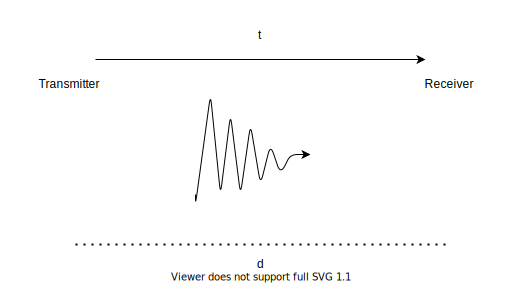
\includegraphics[width=.8\linewidth]{../Photos/toa-oneway.png}\\
      {(a) One-way}
    \end{minipage}%
    % -----------------
    \begin{minipage}{.5\textwidth}
      \centering
      \includegraphics[width=.8\linewidth]{../Photos/toa-roundtrip.png}\\
      {(b) Roundtrip}
    \end{minipage}
    \hfill \break
    \decoRule
    \caption[Περιπτώσεις Time of Arrival]{Περιπτώσεις Time of Arrival} %\caption[Time of Arrival cases]{Time of Arrival cases}
    \label{fig:Time-of-Arrival-cases}
\end{figure}

Μπορούμε να το παρακάμψουμε αυτό, με το να γίνει η μέτρηση σε Round-Trip Time (\Abbr{RTT}), \Fig{Time-of-Arrival-cases} (b).
Σε αυτήν την περίπτωση το ένα node στέλνει ένα σήμα, και μόλις το λάβει ένα γειτονικό node, απαντάει πίσω στο πρώτο. 
Με αυτόν τον τρόπο η μέτρηση του χρόνου εκκίνησης $t_a$ και άφιξης $t_b$ του σήματος γίνονται στο ίδιο node - 
άρα δεν χρειάζεται συγχρονισμός, και η πραγματική απόσταση είναι η μισή από αυτή που θα υπολογιστεί. Ο κύριος παράγοντας
σφάλματος σε αυτή την μέθοδο, είναι ο υπολογισμός του χρόνου που χρειάστηκε το δεύτερο node για να διαχειριστεί
το σήμα που έλαβε και να απαντήσει. Αυτό το internal delay $t_{in}$ μπορεί να είναι είτε γνωστό από 
ένα a priori calibration, είτε μπορεί να μετριέται και να στέλνεται μαζί με το σήμα απάντησης - ώστε να αφαιρείται
από τον χρόνο μετάδοσης του κύματος \cite{wsn-Localization-techniques}.
Με αυτά τα δεδομένα, η σχέση \EqNum{toa-roundtrip} περιγράφει τον τρόπο υπολογισμού της
απόστασης \emph{d} μεταξύ των δύο nodes.

\begin{align}
	d=\frac{s(t_b-t_a-t_{in})}{2} \label{eq:toa-roundtrip}
\end{align}


Όσον αφορά την τεχνική \Abbr{TDoA}, και σε αυτήν την περίπτωση υπάρχουν δύο παραλλαγές της \cite{wsn-Localization-systems} - όπου και οι 
δύο είναι βασισμένες στην αρχή το ότι δεν μας ενδιαφέρει η χρονική στιγμή που ξεκίνησε η αποστολή ενός σήματος, αλλά μόνο
οι χρονική στιγμή που το λάβαμε.

\begin{figure} [H]
    \centering
	% -----------------
    \begin{minipage}{.5\textwidth}
      \centering
      \includegraphics[width=0.8\linewidth]{../Photos/tdoa-multiple.png}\\
      {(a) Single signal - multiple receivers}
    \end{minipage}%
    % -----------------
    \begin{minipage}{.5\textwidth}
      \centering
      \includegraphics[width=.8\linewidth]{../Photos/tdoa-timing.png}\\
      {(b) Multiple signals - single receiver}
    \end{minipage}
    \hfill \break
    \decoRule
    \caption[Περιπτώσεις Time Difference of Arrival]{Περιπτώσεις Time Difference of Arrival} %\caption[Time Difference of Arrival cases]{Time Difference of Arrival cases}
    \label{fig:Time-Difference-of-Arrival-cases}
\end{figure}


Η πρώτη περίπτωση σχετίζεται με single signal και multiple receivers, παρουσιάζεται στην 
\Fig{Time-Difference-of-Arrival-cases} (a), 
χρησιμοποιείται συνήθως στα cellular network και απαιτεί την ύπαρξη 
τουλάχιστον 4 beacons για την απόκτηση location πληροφορίας ενός free node στον τρισδιάστατο χώρο. Υπολογίζει την χρονική διαφορά
που έφτασε σε καθένα από τα beacons το σήμα που έστειλε το free node, για την εκτίμηση της θέσης του free node από
το καθένα από αυτά. Σημαντικό σε αυτήν την περίπτωση είναι και εδώ, να είναι απόλυτα συγχρονισμένα τα beacons. 
Βασίζεται στις ιδιότητες των υπερβολικών καμπύλων και στο ότι με δεδομένη μία συγκεκριμένη χρονική διαφορά του σήματος, 
το free node θα πρέπει να βρίσκεται κάπου πάνω σε μία υπερβολική καμπύλη όπως παρουσιάζεται από την \Fig{TDoA-hyberbolas}
\cite{youtube-angle-of-arrival-tdoa-hyberbolas}. 

Μόνο από αυτόν τον υπολογισμό δεν δύναται να κάνουμε ακριβή εκτίμηση από\-στασης, 
μπορούμε να συμπεράνουμε όμως τον γεωμετρικό τόπο στον οποίο βρίσκεται το free node. Στη \Sect{Multilateration} - και σε επέκταση αυτού -
παρουσιάζεται όμως, ο τρόπος με τον οποίο μπορούμε να συνδυάσουμε τέτοια πληροφορία από πολλαπλά beacon για να εκτιμήσουμε την ακριβή θέση του free node.

\begin{figure} [H]
	\centering
	% -----------------
    \begin{minipage}{.5\textwidth}
      \centering
      \includegraphics[width=0.6\linewidth]{../Photos/tdoa-dt-0.png}\\
      {(a) $Δt = 0$}
    \end{minipage}%
    % -----------------
    \begin{minipage}{.5\textwidth}
      \centering
      \includegraphics[width=0.4\linewidth]{../Photos/tdoa-dt-not-0.png}\\
      {(b) $Δt \neq 0$}
	\end{minipage}
	% -----------------
    \hfill \break
    \decoRule
    \caption[TDoA υπερβολές βασισμένες στο $\Delta t$]{TDoA υπερβολές βασισμένες στο $\Delta t$} %\caption[TDoA hyberbolas based on $\Delta t$]{TDoA hyberbolas based on $\Delta t$}
    \label{fig:TDoA-hyberbolas}
\end{figure}
\begin{align}
	\Delta t = a-a = 0 \quad \quad \quad & \quad \quad \quad\Delta t = x-a \nonumber \\
	\Delta t = b-b = 0 \quad \quad \quad & \quad \quad \quad\Delta t = y-b \nonumber \\
	\Delta t = c-c = 0 \quad \quad \quad & \quad \quad \quad\Delta t = z-c \nonumber
\end{align}


Η δεύτερη εκδοχή της χρήσης \Abbr{TDoA} - η οποία είναι πιο συχνή στα \Abbr{WSN} και 
μας ε\-νδια\-φέ\-ρει περισσότερο, 
χρησιμοποιεί multiple signals με single receiver και παρουσιάζεται στην \Fig{Time-Difference-of-Arrival-cases} (b). 
Αρχή λειτουργίας έχει ότι ο transmitter θα στείλει πολλαπλά - διαφορετικού είδους - σήματα και ο δέκτης θα μετρήσει την χρονική διαφορά 
που τα έλαβε. Ως παράδειγμα μπορεί το ένα σήμα να είναι σε \Abbr{RF} και να κινείται με ταχύτητα $s_r=c_o$ και το άλλο 
ηχητικό με ταχύτητα $s_s \approx 343m/s$ \footnote{Για μετάδοση σε ξηρό αέρα υπό θερμοκρασία \SI{20}{\celsius} \cite{wikipedia-speed-of-sound}}. 
Αν $t_r$ η χρονική στιγμή που λαμβάνει το \Abbr{RF} σήμα, $t_s$ το ηχητικό και $t_d$ το delay που μεσολάβησε από την αποστολή του ενός στο άλλο,
τότε μπορούμε να υπολογίσουμε την απόσταση μεταξύ των κόμβων από την εξίσωση \EqNum{tdoa-distance}
\cite{wsn-Localization-systems} \cite{localization-algorithms}.

\begin{align}
	d=&(s_r-s_s)(t_s-t_r-t_{d}) \label{eq:tdoa-distance}
\end{align}

Θετικό σε αυτήν την μέθοδο είναι ότι το error μπορεί να είναι της τάξης των μερικών εκατοστών, όμως αρχικά απαιτεί επιπλέον εξοπλισμό στο node -
ώστε να μπορεί να στείλει και να λάβει πολλαπλά είδη σήματος - πράγμα που μπορεί να το κάνει αντι\-οι\-κο\-νο\-μι\-κό ή αρκετά μεγαλύτερο σε διαστάσεις από 
το επιθυμητό. Όπως επίσης - και μάλιστα  
σημαντικότερο - η απόσταση η οποία μπορεί να 
χρησιμοποιηθεί, επηρεάζεται σε μεγάλο βαθμό από τα χαρακτηριστικά του δεύτερου σήματος. Ως παράδειγμα, τα ηχητικά σήματα 
δεν μπορούν να μεταφερθούν σε μεγάλες αποστάσεις ή το ότι η ταχύτητα τους μπορεί να επηρεαστεί σημαντικά από περιβαλλοντολογικούς παράγοντες
\cite{farooqiazam2016location}.\footnote{Η συγκεκριμένη μέθοδος είναι διαισθητικά παρόμοια, με αυτό που θα κάναμε για να εκτιμήσουμε 
την απόσταση μίας αστραπής από εμάς, μετρώντας το χρονικό διάστημα μέχρι να ακούσουμε την βροντή.} 

%----------------------------------------------------------------------
\subsubsection{Εκτίμηση γωνίας}\label{sec:Chapter3-1-2} %\subsubsection{Angle}\label{sec:Chapter3-1-2}

Άλλη μία χρήσιμη μέτρηση η οποία μας ενδιαφέρει, είναι η εκτίμηση της γωνίας από την οποία λαμβάνουμε το σήμα ενός γειτονικού
node σε σχέση με έναν άξονας αναφοράς. Ο άξονας αυτός μπορεί να είναι είτε κοινώς για όλα τα nodes (π.χ. ως προς το βόρειο γεωγραφικό πόλο),
είτε μπορεί να είναι για το κάθε node ξεχωριστός, ως παράδειγμα με βάση τον προσανατολισμό του ίδιου του node ή με βάση την γωνία λήψης ενός 
επιπλέον σήματος \cite{wsn-Localization-systems}. Την πληροφορία αυτή την βρίσκουμε στην βιβλιογραφία να ονομάζεται Angle of Arrival 
(\Abbr{AoA}) ή Direction of Arrival (\Abbr{DoA}). 

\begin{align}
	s(t)=A\sin(2\pi ft + \phi) \label{eq:signal-equation}
\end{align}

Γνωρίζουμε ότι ένα σήμα καθορίζεται πλήρως από τρεις παραμέτρους, το πλάτος του A, την συχνότητα του \emph{f} καθώς 
επίσης και από την φάση του $\phi$ - σχέση \EqNum{signal-equation}. Για τον υπολογισμό της γωνίας \Abbr{AoA} μπορούν 
να χρησιμοποιηθούν τεχνικές με γνώμονα τα παραπάνω. 

\subsubsection{Amplitude response}
Ο όρος \emph{Beamforming} \cite{wikipedia-beamforming} χρησιμοποιείται για να περιγράψει το pattern 
της ευαισθησίας του σήματος που στέλνει/λαμβάνει μία \emph{directional antenna} \cite{wikipedia-directionl-antenna}. 
% ή γενικά στην χρήση του μοντέλου της \emph{anisotropy antenna}. 
Το pattern αυτού του τύπου κε\-ραί\-ας, παρουσιάζεται στην \Fig{Typical-anisotropic-antenna-pattern}
\cite{wsn-Localization-techniques} και μπορούμε να χρησιμοποιήσουμε αυτό το χαρακτηριστικό για τον υπολογισμό της \Abbr{AoA}. 
Εάν χρησιμοποιούμε \emph{directional ante\-nna} στον receiver και μπορούμε είτε με μηχανικό είτε με ηλεκτρονικό τρόπο να στρέψουμε
την κεραία σε διάφορες κατευθύνσεις, τότε μπορούμε μετρώντας το πλάτος του σήματος που λαμβάνουμε, να εκτιμήσουμε και την κατεύθυνση του - όπου ιδανικά
βρίσκεται εκεί από όπου έχουμε την μέγιστη τιμή του amplitude του κύματος. Σημαντικές παράμετροι για την εκτίμηση της γωνίας σε αυτήν την περίπτωση, 
είναι επίσης η ευαισθησία του δέκτη καθώς και το width του beam της. 
Λανθασμένη εκτίμηση μπορεί να προκύψει, αν για κάποιο λόγο το πλάτος του σήματος που λαμβάνουμε δεν είναι σταθερό. Σε αυτή την περίπτωση, μία λύση
είναι να χρησιμοποιήσουμε μία δεύτερη - μη κινούμενη - \emph{omnidirectional} κεραία και να κανονικοποιήσουμε τις μετρήσεις της \emph{directional} με βάση τις   
μετρήσεις της δεύτερης \cite{wsn-Localization-techniques}.

% IMAGE
\FigCaptLabelBasedURL{../Images/Theoretical-Background/A-typical-radiation-pattern-of-the-directive-antenna.jpeg}%	Image Path
{Pattern ευαισθησίας της anisotropic κεραίας}%	Caption Text {Typical anisotropic antenna pattern}%
{Typical-anisotropic-antenna-pattern}%	Label used
<0.3>% Scale of image
[wsn-Localization-techniques]%	Based on specific paper 
(https://www.sciencedirect.com/science/article/abs/pii/S1389128606003227) % URL that found

\subsubsection{Phase response}
Άλλος τρόπος υπολογισμού του \Abbr{AoA} είναι με την αξιοποίηση της πληροφορία για την φάση που έχουμε για ένα σήμα. Σε αυτήν την περίπτωση
χρειαζόμαστε ή κεραίες αρκετά μεγαλύτερες από το μήκος κύματος του σήματος που στέλνουμε, ή antenna arrays \cite{wsn-Localization-techniques}. 

Για τα κύματα γνωρίζουμε ότι η διαφορά φάσης $\Delta \phi$ δύο σημείων που απέχουν  
μεταξύ τους $\Delta \chi$ μπορεί να υπολογιστεί από την σχέση \EqNum{phase-different-general} \cite{phase-difference}.

\begin{align}
	\Delta \phi = 2\pi\frac{\Delta \chi}{\lambda} = 2\pi\frac{\Delta t}{T} \label{eq:phase-different-general}
\end{align}

Συνεπώς, αν σχεδιάσουμε ένα antenna array, όπου η κάθε κεραία απέχει από την γειτονική της σε συγκεκριμένη απόσταση \emph{d} και μετρώντας 
το phase difference του σήματος που λαμβάνουμε μεταξύ τους, τότε μπορούμε να υπολογίσουμε την γωνία πρόσληψης της ακτινοβολίας μέσω της 
σχέσης \EqNum{aoa-equation} \cite{wsn-Localization-techniques} \cite{youtube-phase-difference-equation}. Παράδειγμα αυτού\udot βρίσκεται στην \Fig{Antenna-Arrays} (a).
Σε αυτήν την περίπτωση χρησιμοποιούμε \emph{o\-mni\-di\-re\-ctio\-nal} κεραίες και o υπολογισμός της διαφοράς φάσης μπορεί να γίνει
μέσω μετρήσεων \Abbr{TDoA}.

\begin{gather} 
	\phi = \frac{2\pi}{\lambda}d\sin(\theta) \Rightarrow \nonumber \\[2pt]
	\theta = \sin^{-1}\left(\frac{\lambda \phi}{2\pi d}\right) \label{eq:aoa-equation}
\end{gather}

Δεν υπάρχουν όμως μόνο τα linear antenna arrays, μπορούμε να τα σχεδιάσουμε σε διάφορες διατάξεις, 
παράδειγμα μίας εξ' αυτών βρίσκεται στην \Fig{Antenna-Arrays} (b).

\begin{figure} [H]
	\centering
	% -----------------
    \begin{minipage}{.5\textwidth}
      \centering
      \includegraphics[width=0.5\linewidth]{../Photos/aoa-2antennas.png}\\
      {(a) Linear Two Antenna Array}
    \end{minipage}%
    % -----------------
    \begin{minipage}{.5\textwidth}
      \centering
      \includegraphics[width=.7\linewidth]{../Images/Theoretical-Background/The-antenna-array-geometry-a-linear-and-b-circular_W640.jpeg}\\
      {(b) Circular Antenna Array \URI{https://www.researchgate.net/publication/298331796_Adaptive_Array_Beamforming_Using_a_Chaotic_Beamforming_Algorithm/figures}}
	\end{minipage}
	% -----------------
    \hfill \break
    \decoRule
    \caption[Παραδείγματα Antenna Arrays]{Παραδείγματα Antenna Arrays} %\caption[Antenna Arrays examples]{Antenna Arrays examples}
    \label{fig:Antenna-Arrays}
\end{figure}

Η μέθοδος με την αξιοποίηση της σχέσης \EqNum{aoa-equation} λειτουργεί αρκετά καλά όταν έχουμε υψηλό Signal to Noise Ratio (\Abbr{SNR}),
αλλά μπορεί να έχει λανθασμένα αποτελέσματα όταν έχουμε διασυμβολικές παρεμβολές ή multipath signals. 
Επειδή στην πράξη εμφα\-νί\-ζονται και τα δύο, υπάρχει αρκετά μεγάλο επιστημονικό ενδιαφέρον να αντι\-με\-τω\-πι\-στεί αυτός ο περιορισμός.
Αρκετές τεχνικές έχουν προταθεί οι οποίες στρέφονται γύρω από την λογική του Maximum Likelihood (\Abbr{ML})
για τον υπολογισμό τελικά της γωνίας \cite{wsn-Localization-techniques}.

%----------------------------------------------------------------------------------------
%	SECTION 2
%----------------------------------------------------------------------------------------
\subsection{Υπολογισμός θέσης} \label{sec:Chapter3-2} %\subsection{Position Computation} \label{sec:Chapter3-2} 
Αν έχουμε δύο nodes, οι μετρήσεις που λάβαμε από το \Sect{Distance-Angle-Estimation} είναι αρκετές για να γνωρίζουμε την θέση του καθενός,
συνεπώς ενδιαφέρον βρίσκεται στην ύπαρξη τριών ή παραπάνω nodes σε ένα σύστημα. Με βάση τις πληροφορίες που έχουμε συλλέξει - μέσω των τεχνικών που 
περιγράφτηκαν στο προηγούμενο κεφάλαιο - θα προσπαθήσουμε πλέον να εκτιμήσουμε την θέση ενός node. Στην συνέχεια αυτού του section, περιγράφονται μέθοδοι οι οποίοι μπορούν να χρησιμοποιηθούν για να το επιτύχουν
αυτό. Κύρια διαφορά τους είναι η απόδοση που μπορεί να έχουν, η οποία όμως σχετίζεται με την αύξηση της πολυπλοκότητας στους υπολογισμούς που θα
χρειαστούν\udot καθώς επίσης και ποιες από τις παραπάνω πληροφορίες θα εκμεταλλευτούν. 

Για την εύρεση της θέσης ενός unknown node στο τρισδιάστατο χώρο $(\mathfrak{R}^3)$ το Minimal Required number of Sensors (\Abbr{MRS}) είναι τέσσερα nodes.
Στις παρακάτω περιγραφές όμως, και χωρίς βλάβη της γενικότητας θα χρησιμοποιηθούν τρία για την απλούστευση της περιγραφής - με απώτερο σκοπό την εύκολη κατανόηση της, με την παραδοχή ότι μας
ενδιαφέρει η δισδιάστατη ανάλυση $(\mathfrak{R}^2)$. Ενώ στο \Chap{Chapter4} στο οποίο γίνεται και ο σχεδιασμός του συστήματος - βάση συγκεκριμένου αλγόριθμου - 
θα γίνει η ανάλυση στους τρεις άξονες.

%----------------------------------------------------------------------
\subsubsection{Trilateration}\label{sec:trilateration}
Η συγκεκριμένη μέθοδος είναι ίσως η πιο απλή διαισθητικά, βασίζεται στην γεωμετρία κύκλων, είναι αυτή που χρησιμοποιείται από τα \Abbr{GPS}
για τον υπολογισμό θέσης \cite{trilateration-vs-triangulation-video}, ενώ αξιοποιεί μόνο πληροφορία απόστασης και όχι γωνίας \cite{Trilateration-vs-Triangulation}.
Η εξίσωση ενός κύκλου από την γεωμετρία γνωρίζουμε ότι περιγράφεται από την εξίσωση \EqNum{trilateration-circles} όπου $(x_i,y_i)$ οι συντεταγμένες
του κέντρο του κύκλου με ακτίνα $r_i$.

\begin{align}
	(x-x_i)^2 + (y-y_i)^2 &= r_i^2 \label{eq:trilateration-circles}
\end{align}

\begin{figure} [H]
	\centering
    % -----------------
		\begin{minipage}{.5\textwidth}
			\centering
			\includegraphics[width=0.7\linewidth]{../Photos/Trilateration-ideal.png}\\
			{(a) Ideal Trilateration}
		\end{minipage}%
		% -----------------
		\begin{minipage}{.5\textwidth}
			\centering
			\includegraphics[width=.7\linewidth]{../Photos/Trilateration-actual.png}\\
			{(b) Realistic Trilateration}
		\end{minipage}
	% -----------------
    \hfill \break
    \decoRule
    \caption[Παραδείγματα του Trilateration]{Παραδείγματα του Trilateration} %\caption[Trilateration examples]{Trilateration examples}
    \label{fig:Trilateration-examples}
\end{figure}

Εάν χρησιμοποιούμε \emph{omnidirectional κεραίες} \cite{Omnidirectional-antenna} ή στην γενικότερη περίπτωση το μοντέλο της \emph{isotropic antenna} \cite{Isotropic-radiator} και υπολογίσουμε την απόσταση ενός beacon από το node στο οποίο θέλουμε να υπολογίσουμε την θέση του -
τότε μπορούμε να συμπεράνουμε ότι το free node είναι κάπου πάνω στην περιφέρεια ενός 
κύκλου, με κέντρο το beacon και ακτίνα την απόσταση μεταξύ του beacon και του free node. 
Επαναλαμβάνοντας αυτό για ακόμα δύο beacons, τελικά το free node στο δισδιάστατο επίπεδο $(\mathfrak{R}^2)$ θα πρέπει να βρίσκεται στην τομή των τριών κύκλων, πράγμα που γραφικά 
απεικονίζεται στην \Fig{Trilateration-examples} (a) \cite{RSSI-trilateration-Range_based}.

\begin{align}
	x^2-2 x_1 x + x_1^2 + y^2-2 y_1 y + y_1^2 &= r_1^2 \label{eq:trilateration-b1} \\ 
	x^2-2 x_2 x + x_2^2 + y^2-2 y_2 y + y_2^2 &= r_2^2 \label{eq:trilateration-b2} \\
	x^2-2 x_3 x + x_3^2 + y^2-2 y_3 y + y_3^2 &= r_3^2 \label{eq:trilateration-b3} 
\end{align}

Οι εξισώσεις \EqNum{trilateration-b1}, \EqNum{trilateration-b2} και \EqNum{trilateration-b3} περιγράφουν πλήρως τους κύκλους του κάθε node από το παράδειγμα που έχουμε στην \Fig{Trilateration-examples} (a),
όπου $(x_i,y_i)$ το κέντρο του κύκλου, $r_i$ η ακτίνα του - για κάθε beacon $i=1,2,3$ και τελικά $(x,y)$ οι συντεταγμένες του free nodes τις οποίες και ψάχνουμε. 
Ένας τρόπος να υπολογίσουμε τις συντεταγμένες αυτές είναι να αφαιρέσουμε από την \EqNum{trilateration-b2} την \EqNum{trilateration-b1} και όμοια από την 
\EqNum{trilateration-b3} την \EqNum{trilateration-b2} ώστε να καταλήξουμε στις παρακάτω δύο εξισώσεις \cite{trilateration-equations} \cite{localization-algorithms-for-wsn}.

\begin{align}
	(-2x_1+2x_2)x + (-2y_1+2y_2)y = r_1^2 - r_2^2 - x_1^2 + x_2^2 - y_1^2 + y_2^2  \nonumber \\
	(-2x_2+2x_3)x + (-2y_2+2y_3)y = r_2^2 - r_3^2 - x_2^2 + x_3^2 - y_2^2 + y_3^2  \nonumber
\end{align}

Ο λόγος που κάναμε το παραπάνω βήμα είναι διότι πλέον έχουμε ένα σύστημα με δύο εξισώσεις και δύο αγνώστους, οπότε μπορούμε εύκολα να θεωρήσουμε τους παρακάτω πίνακες.

\begin{align}
	A = \begin{bmatrix} -2x_1+2x_2 & -2y_1+2y_2 \\ -2x_2+2x_3 & -2y_2+2y_3 \end{bmatrix} \nonumber \quad
	X = \begin{bmatrix} x \\ y \end{bmatrix} \nonumber \quad
	B = \begin{bmatrix} r_1^2 - r_2^2 - x_1^2 + x_2^2 - y_1^2 + y_2^2 \\ r_2^2 - r_3^2 - x_2^2 + x_3^2 - y_2^2 + y_3^2 \end{bmatrix} \nonumber
\end{align}

Με την χρήση των οποίων καταλήγουμε ότι έχουμε να λύσουμε το γραμμικό σύστημα πινάκων που περιγράφεται από την εξίσωση \EqNum{trilateration-linear-system} για τον
υπολογισμό των συντεταγμένων $(x,y)$ του free node οι οποίες μας ενδιαφέρουν.

\begin{align}
	AX = B \label{eq:trilateration-linear-system}
\end{align}

Όπως αναφέρθηκε και στις προηγούμενες ενότητες, ο υπολογισμός της απόστασης πολύ πιθανόν να περιλαμβάνει μια μικρή απόκλιση $\widehat{r_i} = r_i - ε$, 
με το ε συχνά να θεωρείται μία ανεξάρτητη κανονική τυχαία μεταβλητή με μηδενικό μέσο. Αυτό σημαίνει ότι
τότε οι κύκλοι δεν έχουν ένα κοινό σημείο τομής, αλλά το free node βρίσκεται κάπου μέσα στο χωρίο επικάλυψης
των τριών κύκλων, σχηματικά αυτό παρουσιάζεται στην \Fig{Trilateration-examples} (b) και σε αυτήν την περίπτωση καταλήγουμε σε ένα
μη πεπερασμένο πλήθος λύσεων, με τη συνάρτηση του κάθε κύκλου να περιγράφεται από την εξίσωση
\EqNum{trilateration-circles-error} \cite{wsn-Localization-systems}.

\begin{align}
	(x-x_i)^2 + (y-y_i)^2 &= r_i^2-e \label{eq:trilateration-circles-error}
\end{align}

Το αρνητικό με αυτήν την μέθοδο, είναι η ανάγκη πραγματοποίησης floating point operations για τον υπολογισμό των συντεταγμένων $(x,y)$ σε πραγματικές συνθήκες - όπου το πλήθος
των οποίων εξαρτάται από τον τρόπο που θα επιλέξουμε να επιλύσουμε το σύστημα. 
Μία από τις μεθόδους επίλυσης της γραμμικής εξίσωσης είναι μέσω του least square method, όπου τότε το πλήθος των floating point operations
που απαιτούνται είναι $(m+\frac{n}{3})\cdot n^2$, με $m$ τον αριθμό των αγνώστων και $n$ τον αριθμό των δοθέντων εξισώσεων \cite{wsn-Localization-systems}.

%----------------------------------------------------------------------
\subsubsection{Bounding Box}
Σε αυτήν την μέθοδο χρησιμοποιούνται τετράγωνα αντί για κύκλους του Tri\-la\-te\-ra\-tion, ενώ και εδώ θεωρούμε $(x_i,y_i)$
τις συντεταγμένες των beacon και $d_i$ η από\-στα\-ση που έχουμε υπολογίσει από το free node - για κάθε beacon $i$. 

% IMAGE
\FigCaptLabelBasedURL{../Photos/Bounding-box.png}%
{Bounding Box παράδειγμα}%{Bounding Box example}%
{Bounding-Box-example}%
<0.4>

Δημιουργούμε
τετράγωνα μήκος πλευράς $2d_i$ με κέντρο το κέντρο του beacon και συντεταγμένες $(x_i - d_i, y_i - d_i)$ \& $(x_i + d_i, y_i + d_i)$. 
Θετικό πλέον είναι ότι δεν χρειάζεται να κάνουμε floating point operations για τον υπολογισμό του χωρίου τομής - αλλά μπορούμε να το υπολογίσουμε
με απλή γεωμετρία. Αφού έχουμε υπολογίσει το χωρίο τομής των τετραγώνων μπορούμε να θεωρήσουμε ότι στο κέντρο του βρί\-σκε\-ται το free node.
Παράδειγμα αυτής της μεθόδου βρίσκεται στην \Fig{Bounding-Box-example}.
Η συγκεκριμένη μέθοδος μπορεί να είναι ευκολότερη υπολογιστικά και να απαιτεί λιγότερα processor resources από το Trilateration, όμως ταυτόχρονα 
προκύπτει και μεγαλύτερο σφάλμα απόκλισης \cite{wsn-Localization-systems}.   


%----------------------------------------------------------------------
\subsubsection{Triangulation}
Σε αντίθεση με τις παραπάνω μεθόδους, η τεχνική Triangulation εκτιμάει την θέση του node που μας ενδιαφέρει, χρησιμοποιώντας   
γνώση που έχουμε για γωνίες και όχι εκτίμηση της απόστασης. Ένα απλούστερο παράδειγμα παρουσιάζεται στην \Fig{Principles-of-Triangulation}, όπου σε αυτό το παράδειγμα από την τριγωνομετρία,
μπορούμε εύκολα να συμπεράνουμε ότι για τις γωνίες $\theta_1$ και $\theta_2$ ισχύουν οι σχέσεις \EqNum{angle-equations-triangulation}.

% IMAGE
\FigCaptLabelBasedURL{../Photos/Tringulation-principle.png}%
{Principles of Triangulation}%
{Principles-of-Triangulation}%
<0.4>

\begin{align}
	\theta_1 = \frac{d}{d_1} = tan^{-1}\left(\frac{y_1-y}{x_1-x}\right) \quad \quad \quad
	\theta_2 = \frac{d}{d_2} = tan^{-1}\left(\frac{y_2-y}{x_2-x}\right) \label{eq:angle-equations-triangulation}
\end{align}

Από τις σχέσεις \EqNum{angle-equations-triangulation} μπορούμε να καταλήξουμε στις σχέσεις \EqNum{triangilation-principle} \cite{triangulation-simple-equation}, μέσω 
των οποίων τελικά για δεδομένες θέσεις των beacon - γνωστά δηλαδή τα $(x_i,y_i)$ για κάθε beacon i - και με βάση την μέτρηση των γωνιών $\theta_1$ και $\theta_2$,
να υπολογίσουμε την θέση του free node $(x,y)$.

\begin{equation}
	\begin{gathered}
		x = \frac{y_2 - y_1-  x_2\tan \theta_2 + x_1\tan \theta_1}{\tan \theta_1 - \tan \theta_2} \\[4pt]
		y = x\tan \theta_1 + y_1 - x_1\tan \theta_1 \quad = \quad x\tan \theta_2 + y_2 - x_2\tan \theta_2    
	\end{gathered}
	\label{eq:triangilation-principle}
\end{equation}

\begin{figure} [H]
	\centering
	\hspace*{+2cm}\begin{minipage}{0.4\textwidth}
		\centering
		\includegraphics[width=0.8\linewidth]{../Photos/Tringulation-local.png}\\
		{(a) Local}
	\end{minipage}
	\newline
	\hspace*{+1cm}\begin{minipage}{.4\textwidth}
		\centering
		\includegraphics[width=.8\linewidth]{../Photos/Tringulation-remote.png}\\
		{(b) Remote Ideal}
	\end{minipage}%
	% -----------------
	\begin{minipage}{.4\textwidth}
		\centering
		\includegraphics[width=.8\linewidth]{../Photos/Tringulation-remote-actual.png}\\
		{(c) Realistic}
	\end{minipage}
	\hfill \break \\
	\decoRule
	\caption[Triangulation παραδείγματα]{Triangulation παραδείγματα} %\caption[Triangulation examples]{Triangulation examples}
	\label{fig:Triangulation-examples}
\end{figure}

Αυτή η τεχνική εκτίμησης της θέσης του node, μπορεί να γίνει είτε από τοπικές μετρήσεις του ίδιου του node -
\Fig{Triangulation-examples} (a) - είτε από μετρήσεις γωνιών που κάνουν τα anchors - \Fig{Triangulation-examples} (b)
\cite{wsn-Localization-systems}. Φυσικά σε μία πραγματική εφαρμογή, όπως έχει αναφερθεί παραπάνω, οι μετρήσεις παρουσιάζουν αποκλίσεις 
από τα ιδανικά μοντέλα. Συνεπώς την \Fig{Triangulation-examples} (c) παρουσιάζει σε πιο ρεαλιστικά επίπεδα - συνυπολογίζοντας την ύπαρξη 
των αποκλίσεων - 
το χωρίο στο οποίο με μεγαλύτερη πιθανότητα βρίσκεται το node.

%----------------------------------------------------------------------
\subsubsection{Multilateration} \label{sec:Multilateration}
Η μέθοδος του Multilateration\footnote{To Multilateration μπορεί να αναφερθεί τόσο σε time-synchronous όσο και σε non-synchronous προσέγγιση \cite{multilateration-based-on-timing}. Για την time-synchronous ο όρος αυτός χρησιμοποιείται επίσης σε αναφορά της χρήσης του Trilateration ή του Triangulation με πάνω από 3 beacons \cite{wsn-Localization-systems} \cite{triangulation-simple-equation}. Όμως εδώ συζητάτε η γενικότερη που είναι  η non-synchronous.} (\Abbr{MLAT}), 
έχει ως βάση την γεωμετρία των υ\-πε\-ρβο\-λι\-κών καμπύλων και συχνά μπορεί να βρεθεί επίσης και ως hyperbolic positioning 
στην βιβλιογραφία \cite{multilateration-def} \cite{triangulation-trilateration-multilateration} \cite{wikipedia-multilateration}. Στη \Sect{Distance-Angle-Estimation} 
έγινε αναφορά ότι η χρήση του \Abbr{TDoA} βασίζεται στις υπερβολικές καμπύλες, συνεπώς μπορούμε εύκολα να χρησιμοποιήσουμε
τις μετρήσεις αυτές για τον υπολογισμό της θέσης του free node.

Η γενική ιδέα σε αυτήν την περίπτωση περιγράφεται στην εξίσωση \EqNum{tdoa-multiple} \cite{wsn-Localization-techniques} \cite{simple-tdoa} - και αυτό που 
θέλουμε, είναι να υπολογίσουμε την θέση του $k_t$ (free node) γνωρίζοντας για κάθε δύο διαφορετικά $k_i$ και $k_j$ beacon nodes
την χρονική στιγμή $t_i$ και $t_j$ που έφτασε το σήμα στο καθένα - εάν αυτό κινούταν με ταχύτητα s και το $\norm{\cdot}$ συμβολίζει την ευκλείδεια
απόσταση μεταξύ τους.

\begin{align}
	\Delta t_{ij} \triangleq & t_i - t_j = \frac{1}{s} (\norm{k_i - k_t} - \norm{k_j - k_t}), \quad i \neq j\label{eq:tdoa-multiple}
\end{align}

Αυτό που αναπαριστά ουσιαστικά η σχέση \EqNum{tdoa-multiple} δεν είναι τίποτα άλλο από την προσπάθεια εύρεσης του σημείου τομής των καμπύλων.
Παράδειγμα αυτής της μεθόδου βρίσκεται στην \Fig{Multilateration}.

% IMAGE
\FigCaptLabelBasedURL{../Photos/multilateration.png}%
{Multilateration παραδείγματα}%{Multilateration example}%
{Multilateration}%
<0.4>

%----------------------------------------------------------------------
\subsubsection{Πιθανοκρατικοί μέθοδοι}%\subsubsection{Probabilistic approaches}
Το γεγονός ότι οι μετρήσεις απόστασης και γωνίας σε πραγματικές συνθήκες εμπε\-ριέ\-χουν σφάλματα, έχει ωθήσει στην έρευνα 
probabilistic μεθόδων εκτίμησης τοποθεσίας των free nodes. Αυτού του τύπου οι προσεγγίσεις λαμβάνουν υπόψιν τα μετρικά σφάλματα και συχνά τα μοντελοποιούν ως κανονικές
τυχαίες μεταβλητές. Το μεγάλο μειονέκτημα σε αυτήν την μέθοδο είναι τα μεγάλα υπολογιστικά και χωρικά - για την αποθήκευση των δεδομένων - κόστη \cite{wsn-Localization-systems}. 

\begin{table}[H]
    \caption[Σύνοψη τεχνικών εκτίμησης απόστασης/γωνίας και υπολογισμού θέσης]{Σύνοψη τεχνικών εκτίμησης απόστασης/γωνίας και υπολογισμού θέσης \cite{advantages-disadvantages-toa-tdoa-aoa}} %\caption[Distance/angle estimation techniques and position Computation summary]{Distance/angle estimation techniques and position Computation summary \cite{advantages-disadvantages-toa-tdoa-aoa}}
    \label{tab:Distance/angle-estimation-techniques-and-position-Computation-summary}
	\centering
	\resizebox{1\textwidth}{!}{
		\begin{tabular}{ccccc}
			\toprule
			\textbf{Method} & \textbf{Position Computetion}  & \textbf{Advantages} & \textbf{Disadvantages} & \textbf{Applications} \\
			\midrule
				\Abbr{RSSI} & 
					\*Pos*\ \Centerstack{Trila/Multilteration, \\ Bounding box} & 
					\*Adv*\ \Centerstack{Simple, inexpensive, \\no need for extra hardware, \\synchronization not needed} & 
					\*Dis*\ \Centerstack{Multipath interference, \\\Abbr{NLoS} and enviroment \\can affect readings} & 
					\*App*\ \Centerstack{In sort-distance with \Abbr{LoS} \\applications and low \\accuracy needed (e.g. indoor)} \\ \hline 
				\Abbr{ToA} & 
					\*Pos*\ \Centerstack{Trila/Multilteration, \\Bounding box} & 
					\*Adv*\ \Centerstack{High accuracy} & 
					\*Dis*\ \Centerstack{Need to precisely measure time, \\\Abbr{LoS} is normally assumed, \\more sophisticated design} & 
					\*App*\ \Centerstack{Common in cellular networks\\ or systems assisted by \Abbr{GPS}} \\ \hline
				\Abbr{TDoA} & 
					\*Pos*\ \Centerstack{Multilateration} & 
					\*Adv*\ \Centerstack{High accuracy} & 
					\*Dis*\ \Centerstack{Need for extra hardware \\or precisely synchronized nodes} & 
					\*App*\ \Centerstack{Common in \Abbr{WSN}\\ or systems assisted by \Abbr{GPS}} \\ \hline
				\Abbr{AoA} & 
					\*Pos*\ \Centerstack{Triangulation} & 
					\*Adv*\ \Centerstack{\Abbr{MRS} is two nodes (Ideal $\mathfrak{R}^2$), \\synchronization not needed} & 
					\*Dis*\ \Centerstack{\Abbr{LoS} is normally assumed, \\smart antenna design, \\multipath can affect readings} & 
					\*App*\ \Centerstack{Common in radar scenarios} \\ \hline
			\bottomrule
		\end{tabular}
	}
\end{table}

Στο \Tabl{Distance/angle-estimation-techniques-and-position-Computation-summary} γίνεται σύνοψη των μεθόδων εκτίμησης απόστασης
που αναλύθηκαν παραπάνω, μαζί με τις μεθόδους εκτίμησης θέσης που συχνά συνδυάζονται, καθώς και θετικά/αρνητικά όπως και συχνές τους εφαρμογές. 

%----------------------------------------------------------------------------------------
%	SECTION 3
%----------------------------------------------------------------------------------------
\subsection{Localization Αλγόριθμοι} \label{sec:Chapter3-3} %\subsection{Localization Algorithm} \label{sec:Chapter3-3} 
Στις προηγούμενες ενότητες αναφέρθηκαν κάποιες από τις βασικές τεχνικές που χρησιμοποιούνται, 
προκειμένου να εκτιμηθεί η θέση ενός node στον χώρο. Σε ένα πραγματικό σύστημα όμως, πρέπει να συνυπολογιστούν 
και άλλοι παράγοντες πέρα από - απλά - τον υπολογισμό απόστασης/γωνίας για να καταλήξουμε να αποκτήσουμε location information. 
Για αυτό το λόγο, στο παρόν \emph{Section} παρουσιάζονται επιπλέον πτυχές - του συστήματος - που πρέπει να λάβουμε 
υπόψιν\udot καθώς και αναφορά αλγό\-ρι\-θμων από την υπάρχουσα βιβλιογραφία, με τους οποίους μπορούμε να καλύψουμε αυτές τις
ανάγκες. 

Αφού έχουμε δει τα παραπάνω, αρχικά ας ορίσουμε το localization problem με ένα πιο αυστηρό μαθηματικό φορμαλισμό.
Έστω ότι έχουμε στην διάθεση μας \emph{n} αριθμό από nodes, και για λόγους απλότητας\udot συμμετρικά και όμοια δίκτυα
επικοινωνίας - με εμβέλεια \emph{r} - για κάθε node. Συνεπώς, ένα node \emph{u} επικοινωνεί με το \emph{v} αν και μόνο αν, και το
\emph{v} μπορεί να επικοινωνήσει πίσω στο \emph{u}, τα οποία είναι δια\-σκο\-ρπι\-σμένα σε ένα δισδιάστατο τετραγωνικό
πεδίο - και εδώ γίνεται η θεώρηση για $\mathfrak{R}^2$ ανάλυση - \emph{$Q=[0,s]\times[0,s]$}. 

Τότε μπορούμε να μοντελοποιήσουμε το δίκτυο από nodes, ως ένα μη κατευθυνόμενο γράφο $\mathcal{G} = (V, E)$ - παράδειγμα του οποίου υπάρχει στην \Fig{Graph-example} - με τα 
παρακάτω χαρακτηριστικά \cite{wsn-Localization-systems}.  

\begin{itemize}
	\item $V = \{v_1, v_2, ..., v_n\}$ το σύνολο των nodes, όπου έχει την έννοια των κορυφών του γράφου, με $|V| = n$\footnote{Ο 
	παραπάνω συμβολισμός $|\cdot|$ χρησιμοποιείται ως το cardinality του εκάστοτε set}.
	\item $\langle i,j\rangle \in E$ εάν το $u_i$ μπορεί να επικοινωνήσει με το $v_i$. Πράγμα που σημαίνει - με βάση τα παραπάνω - 
	ότι η ευκλείδεια απόσταση τους\udot είναι μικρότερη από \emph{r} και έχει την έννοια των ακμών του γράφου, με $|E| = m$\footnotemark[\value{footnote}].
	\item $0 \le w(e) \le r$ με $e = \langle i,j\rangle$, να είναι το βάρος της κάθε ακμής και να χρησιμοποιείται για την έννοια της απόστασης $d_{ij}$
	μεταξύ του node $u_i$ με το $v_i$.
\end{itemize}

% IMAGE
\FigCaptLabelBasedURL{../Photos/localization-graph.png}
{Παράδειγμα γράφου}%{Graph example}%
{Graph-example}%
<0.4>

%----------------------------------------------------------------------
\subsubsection{One-hop vs Multi-hop}
Η πρώτη κατηγοριοποίηση στην οποία θα αναφερθούμε - για αυτό το δίκτυο γράφου - προκειμένου να εκτιμήσουμε την θέση των nodes, 
είναι από ποιους κόμβους τελικά θα αξιοποιήσουμε πληροφορία. Στους αλγόριθμους \textbf{One-hop} αξιοποιείται πληροφορία,
μόνο από άμεσους γείτονες των nodes\udot προκειμένου να υπολογίσουμε την θέση του κόμβου στο χώρο. Αντίθετα 
στις τεχνικές \textbf{Multi-hop}, χρησιμοποιούμε και πληροφορία που λαμβάνουμε με έμμεσο τρόπο\udot
από τους γείτονες των γειτόνων μας - προκειμένου να αποφανθούμε για την θέση ενός node.

%----------------------------------------------------------------------
\subsubsection{Anchor-based vs Anchor-free}
Ένας ακόμα σημαντικός διαχωρισμός είναι η ύπαρξη ή όχι τελικά στο δίκτυο - από anchor nodes. Καθώς υπάρχουν εφαρμογές
στις οποίες μπορεί να μην χρειάζεται ή να μην έχουμε δυνατότητα να τοποθετηθούν beacons - ακόμα και αν αναφερόμαστε σε mobile beacons -
οπότε τότε θα χρησιμοποιήσουμε \textbf{Anchor-free} αλγορίθμους. Αν υπάρχει η δυνατότητα χρήσης τους, τότε ενδιαφερόμαστε για
\textbf{Anchor-based}.

%----------------------------------------------------------------------
\subsubsection{Relative vs Absolute Positioning}
Ανάλογα με τις προδιαγραφές της εφαρμογής που θέλουμε να καλύψουμε, θα πρέπει να χρησιμοποιήσουμε ανάλογες εκτιμήσεις θέσεων.
Υπάρχουν εφαρμογές, όπως για παράδειγμα - εκτίμηση θέσης των nodes ενός κινούμενου swarm\udot για χαρτογράφηση σε άγνωστο terrain. Σε αυτού 
του τύπου τις εφαρμογές μας ενδιαφέρει η απόλυτη θέση στον χώρο\udot οπότε θέλουμε μεθοδολογίες για \textbf{Absolute Positioning}, ενώ 
υπάρχουν άλλες εφαρμογές στις οποίες μας ενδιαφέρει μόνο πληροφορία θέσης σε σχέση με τα υπόλοιπα στοιχεία του περιβάλλοντος της
εφαρμογής, οπότε χρειαζόμαστε \textbf{Relative Positioning}.

%----------------------------------------------------------------------
\subsubsection{Indoor vs Outdoor Scenarios}
Κάτι ακόμα που πρέπει να προσέξουμε είναι το περιβάλλον στο οποίο θα βρίσκεται η εφαρμογή, καθώς ανάλογα με το περιβάλλον\udot
έχουμε να διαχειριστούμε και τις δυσκολίες που μας παρουσιάζει - εμπόδια, ανακλάσεις σημάτων, κλπ. Με δύο κύριους διαχωρισμούς,
τα \textbf{Indoor Scenarios} και τα \textbf{Outdoor Scenarios}.

%----------------------------------------------------------------------
\subsubsection{Distributed vs Centralized Position Computation}
Πρέπει να αναφερθεί επίσης, ότι είναι πολύ σημαντικό να είναι ξεκάθαρο το σημείο\udot στο οποίο
θα γίνεται η επεξεργασία της πληροφορίας. Υπάρχουν δύο ενδεχόμενα. Το πρώτο
είναι, ένα \Abbr{BS} να αντιλαμβάνεται και να υπολογίζει την θέση των nodes, τα οποία
έπειτα θα ενημερώνονται μέσω αυτού\udot για την θέση τους - οπότε αναφερόμαστε για \textbf{Centralized} τεχνικές. Αντίθετα άλλη εναλλακτική 
είναι να γίνει τοπικά η επεξεργασία. Σε αυτή την περίπτωση, αναφερόμαστε για \textbf{Decentralized} ή \textbf{Distri\-bu\-ted} αλγορίθμους\udot όπου κάθε node θα 
επικοινωνεί από μόνο του με τα γειτονικά του για την απόκτηση πληροφορίας\udot και έπειτα υπολογίζει μεμονωμένα την θέση του. 
Το μεγάλο πλεονέκτημα των Centralized αλγορίθμων είναι ότι απομακρύνουμε το πρόβλημα του computation από το κάθε node, όμως την ίδια στιγμή
προκύπτουν δυσκολίες όπως καθυστερήσεις στις επικοινωνίες, μεγαλύτερο power consumption \& bandwidth, ενώ τέλος
και προβλήματα με το scalability του συστήματος - καθώς προτείνεται για μικρότερα networks. Το οποίο όμως σε ένα βαθμό\udot μπορεί να λυθεί
με το να χρησιμοποιηθούν πολλαπλά \Abbr{BS}s, συνεπώς να έχουμε ένα multi-tier network.
Γνωστοί Centralized αλγόριθμοι είναι o Multi Dimensional Scaling-Mobile Assisted Programming (\Abbr{MDS-MAP}), 
Semi Definite Programming (\Abbr{SDP}) και Localization Based on Simulated Annealing (\Abbr{LBSA}) \cite{range-distributed}.
Παρακάτω στον \Algo{MDS-MAP} - ως παράδειγμα
χρήσης των \emph{Centralized} αλγορίθμων - παρουσιάζεται ο pseudo-code του \Abbr{MDS-MAP}.

\begin{algorithm}[H]
	\caption[Multi Dimensional Scaling-Mobile Assisted Programming]{Multi Dimensional Scaling-Mobile Assisted Programming \cite{localization-algorithms}}\label{alg:MDS-MAP}
	\begin{algorithmic}[1]	% For line numbering just uncomment [1]
		\Statex{{\bf procedure} MDS-MAP ($r_{i,j} = w(e) \quad \forall \quad e \in E$)}
			\State Form a sparse matrix R from $r_{i,j}$
			\State Run a standard all pairs shortest path algorithm on R to produce \newline inter-node distances D (e.g. Dijkstra's, Floyd's)
			\State Run classical metric MDS on D to find estimated positions X
			\State Transform the solution X into global coordinates G
	\end{algorithmic}
\end{algorithm}

\begin{table}[H]
    \caption[Σύγκριση μεταξύ Centralized και Distributed]{Σύγκριση μεταξύ Centralized και Distributed \cite{localization-algorithms-comparizon-tables}} %caption[Comparison of Centralized vs Distributed]{Comparison of Centralized vs Distributed \cite{localization-algorithms-comparizon-tables}}
	\label{tab:Comparison-of-Centralized-vs-Distributed}
	\centering
	\resizebox{0.7\textwidth}{!}{
		\begin{tabular}{lll}
			\toprule
			 & \textbf{Centralized} & \textbf{Distributed}\\
			\midrule
				Accuracy & Data collection & Position merging \\ 
				Energy consumption & Signal transition & Position merging \\ 
				Coverage area & Network topology & Anchor deployment \\ 
				Costs & Central module & Anchor equipment \\ 
			\bottomrule
		\end{tabular}
	}
\end{table}

% \begin{algorithm}[H]
% 	\caption{Localization Based on Simulated Annealing \cite{simulated-annealing} \cite{sal-localization}}\label{alg:LBSA}
% 	\begin{algorithmic}[1]
% 		\Statex{{\bf procedure} LBSA}($r_{i,j} = w(e) \quad \forall \quad e \in E$)
% 			\State Establishing an appropriate objective function $f(x)$
% 			\State Randomly and uniformly place nodes in a square region of side length L
% 	\end{algorithmic}
% \end{algorithm}

%----------------------------------------------------------------------
\subsubsection{Range-based vs Range-free}
Στη \Sect{Energy-based} αναλύθηκαν τεχνικές εκτίμησης απόστασης ή γωνίας μεταξύ των nodes - συγκεκριμένα οι
\Abbr{RSSI}, \Abbr{ToA}, \Abbr{TDoA} και \Abbr{AoA}.
Σε αυτήν την περίπτωση, όταν χρησιμοποιούμε δηλαδή έξτρα hardware ή γενικά\udot εκτεταμένες ranging τεχνικές 
για να καταλήξουμε στις θέσεις των free nodes στον χώρο, αναφερόμαστε σε \textbf{Range-based} μεθόδους.
Θετικό σε αυτήν την περίπτωση είναι ότι έχουμε μεγαλύτερη ακρίβεια της θέσης, όμως ταυτόχρονα 
πιθανόν να χρειαστούμε ακριβότερα nodes - λόγο των έξτρα components ή του πιο \emph{sophisticated hardware}.  

Για να το αποφύγουμε αυτό, μπορούμε να χρησιμοποιήσουμε τεχνικές οι οποίες ονομάζονται \textbf{Range-free}. 
Αυτές οι τεχνικές δεν απαιτούν κανένα επιπρόσθετο hardware, διότι δεν χρησιμοποιούν εκτιμήσεις απόστασης/γωνίας, συνεπώς έχουμε μικρότερο κόστος ανά node. 
Έχουν αρκετό ενδιαφέρον λόγω της απλότητας τους\udot παρά την μικρότερη ακρίβεια που παρέχουν. Γνωστοί Range-free αλγόριθμοι είναι 
ο Approximate Point in Triangle (\Abbr{APIT}), 
Distance Vector-Hop (\Abbr{DV-Hop}), Centroid και Gradient \cite{range-distributed}.
Όμοια με παραπάνω, στους \Algo{APIT} και \ref{alg:DV-Hop} παρουσιάζονται οι pseudo-codes 
των \Abbr{APIT} και \Abbr{DV-Hop} αντίστοιχα.

% ALGORITHM
\begin{algorithm}[H]
	\caption[Approximate Point in Triangle]{Approximate Point in Triangle \cite{localization-algorithms}}\label{alg:APIT}
	\begin{algorithmic}[1]
			\Statex{{\bf procedure} APIT}
			\State Receive beacon positions from hear-able beacons.
			\State Initialize inside-set to be empty
			
			\For{each triangle $T_i$ in possible triangles formed over beacons}
				\State Add $T_i$ to inside-set if node is inside $T_i$.
					Go to next Step when accuracy
					\newline\hspace*{1.5em}of inside-set is sufficient.
			\EndFor
			
			\State Compute position estimate as the center of mass of the intersection of all 
			\newline triangles in inside-set.	
	\end{algorithmic}
\end{algorithm}

% ALGORITHM
\begin{algorithm}[H]
	\caption[Distance Vector-Hop]{Distance Vector-Hop \cite{dv-hop-algo} \cite{dv-hop-algo2} \cite{dv-hop-algo3}}\label{alg:DV-Hop}
	\begin{algorithmic}[1]
		\Statex{{\bf procedure} DV-Hop}{}
			
			\For{Each anchor}
				\State Broadcast a message with it's ID, location and hop count initialized to 0
      		\EndFor 
			
			\For{all nodes received all messages from neighbors}
				\State Neighbor nodes record the node ID, the coordinate values, and  the smallest  
				\newline\hspace*{1.5em}hop. Then forward packet after incrementing hop by one
      		\EndFor

			\For{each anchor i to each anchor j}
				\State Estimate Average Hop Distance (\Abbr{AHD}) \par
				\hspace*{7em}$HopSize_i = \frac{\sum{\sqrt{(x_i-x_j)^2+(y_i-y_j)^2}}}{\sum{hop_{i,j}}}, i\neq j$

				\State Broadcast \Abbr{AHD} to network
			\EndFor
			
			\For{each free node u}
				\State Save the first \Abbr{AHD} you hear, then broadcast it to your neighbors 
				\State Calculate your distance from your closest anchor \emph{k},
				$d_{uk} = HopSize_i \times hop_{uk}$
			\EndFor

			\State Based on known beacons' coordinates and estimated distances, use one of the methods described in 
			\emph{Section} \getLabel{sec:Chapter3-2} to compute free nodes locations
	\end{algorithmic}
\end{algorithm}

% TABLE
\begin{table}[H]
    \caption[Σύγκριση μεταξύ Range-based και Range-free]{Σύγκριση μεταξύ Range-based και Range-free \cite{localization-algorithms-comparizon-tables}} %\caption[Comparison of Range-based vs Range-free]{Comparison of Range-based vs Range-free \cite{localization-algorithms-comparizon-tables}}
	\label{tab:Comparison-of-Range-based-vs-Range-free}
	\centering
	\resizebox{0.7\textwidth}{!}{
		\begin{tabular}{lll}
			\toprule
			 & \textbf{Range-based} & \textbf{Range-free}\\
			\midrule
				Accuracy & Ranging algorithm & Geometric algorithm \\ 
				Energy consumption & Signal transition & Instruction execution \\ 
				Coverage area & Signal cover & Network topology \\ 
				Costs & Ranging module & Execution module \\ 
			\bottomrule
		\end{tabular}
	}
\end{table}



% Horizontal Line
% \HLineWithSpaces<2>[300]<2>

Σε ευρύτερη κλίμακα, στην βιβλιογραφία υπάρχουν επιπλέον αλγόριθμοι ή παραλλαγές χρήσης αυτών που αναφέρθηκαν, για την εύρεση τοποθεσίας
nodes σε ένα \Abbr{WSN}. Παρόλα αυτά, σε αυτό το σημείο έγινε μία συνοπτική αναφορά τους,  και μία πρώτη
ανάλυση γύρω από το localization problem. Στην συνέχεια,
με βάση αυτές τις αρχές\udot θα γίνει η μοντελοποίηση του συστήματος που συσχετίζεται αυτή η διπλωματική. 

% ----------------------------------------------------------------------------------------------------------------------------------------------------------
\section{Εκτίμηση Θέσης με οπτικούς τρόπους} \label{chap:Image-based} %\section{Image-based Position Estimation} \label{chap:Image-based}
Άλλος ένας τρόπος για να καταλήξουμε να εκτιμήσουμε την θέση ενός αντικειμένου στον χώρο\udot είναι με την βοήθεια καμερών και οπτικών τεχνολογιών. Κύριος πε\-ριο\-ρι\-στι\-κός παράγοντας σε αυτές τις προσεγγίσεις, είναι η ανάγκη για οπτική επαφή με το αντικείμενο ενδιαφέροντος. Ενώ, καταλήγει να είναι και ο τρόπος με τις μεγαλύτερες ανάγκες επεξεργασίας. Βασικοί τρόποι απόκτησης \Abbr{3D} πληροφορίας - με χρήση \Abbr{2D}, που προσφέρει τυπικά μία κάμερα\footnote{Σε αντίθεση με τις RGB-D, οι οποίες εκτός από color information, παρέχουν και depth information για κάθε pixel τους} - είναι μέσω τεχνικών με όνομα structure from reference, structure from motion και με χρήση stereo \cite{location-from-image} οι οποίες συνοπτικά αναλύονται στην συνέχεια.

%----------------------------------------------------------------------
\subsection{Structure from Reference} \label{sec:theo-structure-from-reference}
Τυπικά, κατά τη μεταφορά των σημείων του πραγματικού κόσμου \Abbr{3D} σε pixel μίας εικόνας \Abbr{2D} χάνουμε την διάσταση του βάθους, πράγμα που μπορεί να δημιουργήσει πλάνες/αυταπάτες - παράδειγμα αυτού στην \Fig{depth-ambiguity-optical-illusion}. Ένας τρόπος για την επανάκτηση της πληροφορίας του depth - προκειμένου να εκτιμήσουμε μέσω εικόνας την θέση των αντικειμένων - είναι με το να υπάρχουν στο scene αντικείμενα γνωστών διαστάσεων, τα οποία θα χρησιμοποιηθούν ως reference objects.

\begin{figure} [H]
	\centering
    % -----------------
		\begin{minipage}{.4\textwidth}
			\centering
			\captionsetup{width=.9\linewidth}
			\includegraphics[width=0.8\linewidth]{../Images/Theoretical-Background/Two-well-known-optical-illusions-where-the-actual-depth-order-of-the-scene-objects-is.jpg}\\
			\decoRule
			\CaptionBasedwithURL{Optical illusion που δημιουργείται λόγο του depth ambiguity}%\CaptionBasedwithURL{Optical illusion due to depth ambiguity of scene objects}
			(https://www.researchgate.net/figure/Two-well-known-optical-illusions-where-the-actual-depth-order-of-the-scene-objects-is_fig4_285270806)
			\label{fig:depth-ambiguity-optical-illusion}
		\end{minipage}%
		% -----------------
		\begin{minipage}{.6\textwidth}
			\centering
			\includegraphics[width=\linewidth]{../Images/Theoretical-Background/Lens_angle_of_view.png}\\
			\decoRule
			\CaptionBasedwithURL{Optical axis του αντικειμένου - κάμερας}%\CaptionBasedwithURL{Optical axis from object to camera sensor}%
			(https://en.wikipedia.org/wiki/Angle\_of\_view) 
			\label{fig:optical-axis-from-object-to-camera-sensor}
		\end{minipage}
	% -----------------
    % \hfill \break
\end{figure}

Στην \Fig{optical-axis-from-object-to-camera-sensor} παρουσιάζονται οι νοητές ευθείες πορείας του φωτός στο thin lens model, από τα σημεία του τρισδιάστατου κόσμου, προς τον αισθητήρα της κάμερας. Όπου $S_1$ η απόσταση του αντικειμένου από την κάμερα σε $m$, $S_2$ η απόσταση του image plane για το pinhole model (περισσότερες πληροφορίες στη \Sect{design-implementation-camera}) σε $mm$, $F$ το focal length σε $mm$, $d$ το μέγεθος του αντικειμένου στην εικόνα σε $mm$ και $H$ το μέγεθος του αντικειμένου στον πραγματικό κόσμο σε $m$. Επίσης, θεωρούμε ότι το αντικείμενο είναι σε focus, συνεπώς $F=S_2$. Τότε, με χρήση τριγωνομετρίας και όμοιων τριγώνων τόσο από την μεριά του αισθητήρα, όσο και του αντικειμένου, καταλήγουμε στην σχέση \EqNum{distance-from-object-dim-triangles} \cite{calculate-distance-or-size-of-an-objectin-a-photo-image} \cite{calculate-distance-opencv} \cite{calculate-distance-stackexchange}.

\begin{align}
	\frac{d}{F} &= \frac{H}{S_1} \label{eq:distance-from-object-dim-triangles}
\end{align}

Από την οποία καταλήγουμε στην \Equa{distance-from-object}. Όπου στο μέγεθος του α\-ντι\-κει\-μέ\-νου μπορούμε να χρησιμοποιήσουμε οποιαδήποτε διάσταση επιθυμούμε, όπως το ύψος, το πλάτος ή ακόμα και κάποια διαγώνιο του.

\begin{align}
	\textrm{Distance to object $S_1$ (m)} &= \textrm{Focal length $F$ (mm)}\frac{\textrm{Object real size $H$ (m)}}{\textrm{Object size on sensor $d$ (mm)}} \label{eq:distance-from-object}
\end{align}

Σε γενικές γραμμές η αναδόμηση της τρίτης διάστασης από single view ακόμα και με ύπαρξη γνωστών αντικειμένων στο scene, μπορεί να καταλήξει να είναι μία ε\-ξαι\-ρε\-τι\-κά ασαφής διαδικασία. Για αυτό τον λόγο προσπαθούμε είτε μέσω monocular vision να πάρουμε πολλαπλά views ενός κινούμενου αντικειμένου και να χρησιμοποιήσουμε τεχνικές με όνομα Structure from Motion (βλ. \Sect{theo-structure-from-motion}), είτε από πολλαπλές κάμερες - stereo vision (βλ. \Sect{theo-stereo}) - να λάβουμε πολλαπλά views στατικού αντικειμένου για την εκτίμηση τελικά του depth. 

%----------------------------------------------------------------------
\subsection{Structure from Motion} \label{sec:theo-structure-from-motion}
Αρχή λειτουργίας της μεθόδου Structure from Motion, είναι η εξαγωγή features από ένα image frame και το tracking τους κατά την διάρκεια κίνησης της κάμερας. Με αυτόν τον τρόπο, στο τέλος της διαδικασίας - για το δοθέν sequence of frames - συλλέγεται ένα σύνολο σημείων για κάθε feature $p_{f} = (x_{f}, y_{f})$ στο image plain της κάμερας (για κάθε frame f) τα οποία αναπαριστούν το ίδιο σημείο στο φυσικό κόσμο $P = (x,y,z)$. Η \Fig{structure-from-motion-example} αναπαριστά παράδειγμα αυτής της διαδικασίας. Αφού συλλεχθούν τα παραπάνω δεδομένα, μπορούν να περάσουν από μία πληθώρα γκάμα αλγορίθμων με ομώνυμο όνομα, μέσω των οποίων μπορεί να προσεγγιστεί η τρισδιάστατη μορφή του αντικειμένου, η κίνηση της κάμερας ή άλλες σημαντικές πληροφορίες.

% IMAGE
\FigCaptLabelBasedURL{../Images/Theoretical-Background/sfm-exp.png}%
{Τυπικό παράδειγμα κίνησης εικόνας για ανακατασκευή μέσω Structure from Motion της σκηνής}%
{structure-from-motion-example}%
<0.7>%
(https://speciale.ar/publication/privacypreservingsfm/)


%----------------------------------------------------------------------
\subsection{Stereo Vision} \label{sec:theo-stereo}
Για τον υπολογισμό του depth με χρήση stereo vision, λαμβάνουμε από δύο κάμερες views ενός scene. Σε γενίκευση τα image planes μπορεί να έχουν οποιαδήποτε προσανατολισμό, ειδική περίπτωση - και συχνά πιο χρησιμοποιούμενη - είναι αυτή που υπάρχει στην \Fig{stereo-vision} (a) στην οποία είναι παράλληλα. Προκειμένου να εκτιμηθεί το depth με χρήση stereo γίνονται υπολογισμοί βασισμένοι στο Epipolar Geometry \cite{wiki-epipolar-geometry}.

\begin{figure} [H]
	\centering
    % -----------------
		\begin{minipage}{.5\textwidth}
			\centering
			% \captionsetup{width=.9\linewidth}
			\includegraphics[width=\linewidth]{../Images/Theoretical-Background/Stereo-vision-principle.png}\\
			{(a) Stereo Vision Principle \URI{https://www.researchgate.net/figure/Stereo-vision-principle-two-cameras-which-view-the-same-scene-detect-a-common-3D-point_fig1_221908788}}
		\end{minipage}%
		% -----------------
		\begin{minipage}{.5\textwidth}
			\centering
			\includegraphics[width=\linewidth]{../Photos/stereo-math.png}\\
			{(b) Stereo Vision Geometry}
		\end{minipage}
	% -----------------
    \hfill \break \\
	\decoRule
	\caption[Stereo Vision]{Stereo Vision}
	\label{fig:stereo-vision}
\end{figure}

Η \Fig{stereo-vision} (b) παρουσιάζει την γεωμετρία στην περίπτωση των parallel optical axis. Μέσω σχέσεων των όμοιων τριγώνων $(p_l, P, p_r)$ και $(COP_L, P, COP_R)$ μπορούμε να δημιουργήσουμε την σχέση \EqNum{stereo-basic-eq}, από την οποία τελικά καταλήγουμε στην \Equa{stereo-depth-est} για τον υπολογισμό του depth ενός Point \cite{introduction-to-computer-vision}. 

\begin{gather}
	\frac{B-x_l+x_r}{Z-F} = \frac{B}{Z} \Rightarrow \label{eq:stereo-basic-eq} \\
	Z = F \frac{B}{x_l - x_r} \label{eq:stereo-depth-est}
\end{gather}

Η ποσότητα $x_l - x_r$ ονομάζεται Disparity, και ουσιαστικά μετρώντας την διαφορά της θέσης που εμφανίζεται στο κάθε plane το point, υπολογίζουμε την απόσταση του σημείου από το baseline των καμερών \cite{introduction-to-computer-vision}.

% This should be the last section
\section{Σκοποί Διπλωματικής} \label{chap:thesis-approach} %\section{Thesis Approach} \label{chap:thesis-approach}
Σκοπός της παραπάνω βιβλιογραφικής αναζήτησης\udot ήταν η απόκτηση μίας σφαιρικής γνώσης σχετικά με τους δυνατούς τρόπους επίλυσης του προβλήματος εντοπισμού της θέσης αντικειμένων, ώστε να πραγματοποιηθεί μία αρχική εκτίμηση της πολυπλοκότητας και του κόστους hardware που απαιτεί η κάθε μία, προκειμένου τελικά να γίνει η επιλογή της μεθοδολογίας με την οποία θα υλοποιηθεί στην συγκεκριμένη εργασία\udot η επίλυση του προβλήματος ενδιαφέροντος.

Φυσικοί περιορισμοί, προκύπτουν από τις δυνατότητες του διαθέσιμου εξοπλισμού που υπάρχουν στο \href{https://www.tuc.gr/}{Πολυτεχνείο Κρήτης}, βάση των οποίων θα γίνει και ο σχεδιασμός του συστήματος. Πράγμα που καθιστά το σύστημα να ακολουθεί ρεα\-λι\-στι\-κά requirements, τον σχεδιασμό με γνώμονα την επίλυση ενός πραγματικού προ\-βλή\-ματος, όπως επίσης και την δυνατότητα - με αυτόν τον τρόπο - να υπάρχουν δυνατότητες δοκιμών από αυτά, σε περίπτωση που χρειαστεί. 

Ακολουθώντας την λογική των \Abbr{MoCap} system (βλ. \Sect{related-motion-capturing-systems}). Στην συ\-γκε\-κρι\-μέ\-νη διπλωματική εργασία γίνεται μία πρώτη προσπάθεια επίλυσης του προ\-βλή\-μα\-τος υπολογισμού της θέσης ενός μεμονωμένου - γνωστών διαστάσεων - α\-ντι\-κει\-μένου με
χρήση drones swarm που πραγματοποιεί close formation flight, όπως παρουσιάζεται στην \Fig{thesis-system-overview} με σκοπό μελλοντικά να
χρησιμοποιηθούν ως feature points και να είμαστε πιο κοντά σε ένα Cooperative Localization (\Abbr{CL}) Real Time Location System (\Abbr{RTLS}) για εντοπισμό και ανίχνευση της θέσης αντικειμένων σε εξωτερικούς χώρους και δυναμικά περιβάλλοντα.

% IMAGE
\FigCaptLabelBasedURL{../Photos/3dDrones-camera-pose.png}%
{Thesis drone swarm system overview}%
{thesis-system-overview}%
<0.5>

Παρόμοια προβλήματα προσπαθούν να λύσουν στην έρευνα τους \cite{theo-human-motion} οι οποίοι με ένα μεμονωμένο drone προσπαθούν να πραγματοποιήσουν Human \Abbr{MoCap}. Επίσης, οι συγγραφείς του \cite{theo-swarm-localiza-and-track-object} χρησιμοποιούν τρία quad-copter για να πραγματοποιήσουν Localization and Tracking ενός αντικειμένου. Στην συγκεκριμένη διπλωματική δίνεται έμφαση όμως στα παρακάτω.

Το σύστημα που σχεδιάζεται στα επόμενα κεφάλαια, είναι προσανατολισμένο να χρησιμοποιείται από Multirotor
drones (βλ. \Sect{Chapter1-1-1}), τα οποία θα κινούνται με σχετικά χαμηλές ταχύτητες και μπορούν να πραγματοποιήσουν hover σε αυθαίρετες θέσεις περιφερειακά του
αντικειμένου που θέλουμε να εντοπίσουμε στον \Abbr{3D} space, χωρίς την a priori ανάγκη γνώσης της θέσης τους, 
παρόλα αυτά το rotation τους (βλ. \Sect{Chapter1-1-1}) - για λόγους ευκολία σχεδίασης - θα θεωρηθεί ότι είναι ήδη με κατεύθυνση
το αντικείμενο ενδιαφέροντος.

Κύρια σημεία αναφοράς, είναι αρχικά να επιτευχθεί relative positioning του αντικειμένου με real time onboard sensing and computing, με την βοήθεια ενός Embedded Linux System.
Άρα πρόκειται να σχεδιαστεί ένα Anchor-based, One-hop και Range-based σύστημα για μελλοντική χρήση σε Outdoor Scenarios το οποίο 
προσπαθεί να επιτύχει Online Distributed Position Computation (βλ. \Sect{Chapter3-3}).

Η εκτίμηση της απόστασης του αντικειμένου από το κάθε drone θα γίνει με χρήση monocular
vision - από την στιγμή που αποτελεί ένα ετερογενές κομμάτι του συστήματος - όπου αφού εντοπιστεί, ακολουθούνται τεχνικές σχετικά με τις γνώσεις των ακριβών του διαστάσεων και τις λαμβανόμενες από την κάμερα μετρήσεις (βλ. \Sect{theo-structure-from-reference}) για να υπολογιστούν τα ranges
του αντικειμένου από το κάθε drone, τα οποία στην συνέχεια θα χρησιμοποιηθούν στον Range-based αλγόριθμο ώστε να πραγματοποιηθεί το position computation (βλ. \Sect{Chapter3-2}).
   % Related Work
\chapter{Design Features and Implementation} % Main chapter title
\label{chap:Chapter4}  % For referencing the chapter elsewhere, use \ref{Chapter4}

\epigraph{”Our goals can only be reached through a vehicle of a plan, in which we must fervently believe, and upon which we must vigorously act. There is no other route to success." }{\textit{Pablo Picasso}}

Στο παρόν κεφάλαιο περιγράφεται η διαδικασία σχεδιασμού και υλοποίησης του \Abbr{MoCap} με χρήση drone swarm συστήματος, που συσχετίζεται η παρούσα διπλωματική. 

Μία high-level προσέγγιση, θα μπορούσε να διαχωρίζει το σύστημα σε τρία διακριτά
υποσυστήματα. Αρχικά το optical, του οποίου αρμοδιότητα είναι το detection, το tra\-cking, καθώς και η εκτίμηση
του range ή γωνίας του αντικειμένου από την camera. Δεύτερο, η λήψη των πληροφοριών από τους αισθητήρες ώστε να προσεγγιστεί η θέση του ίδιου
του drone. Τέλος, ο συνδυασμός των δύο παραπάνω μερών και η χρήση κατάλληλης localization τεχνικής για να βρεθεί η θέση του αντικειμένου
στο \Abbr{3D} χώρο.

%----------------------------------------------------------------------
\section{Equipment and Tools Used} \label{sec:design-tools}
Αρχικά θα αναφερθούν συνοπτικά η αρχιτεκτονική στην οποία έγινε επιλογή να επιλυθεί το πρόβλημα,
όπως επίσης και τα εξαρτήματα/αισθητήρια όργανα καθώς και τα λογισμικά τα οποία χρησιμοποιήθηκαν στην παρούσα διπλωματική. 

\subsection{Embedded Linux System}
Δύο πολύ δημοφιλείς επιλογές στον χώρο των ενσωματωμένων συστημάτων - ως κεντρικές μονάδες επεξεργασίας - είναι οι πλακέτες Raspberry Pi που κατασκευάζονται από την Raspberry Pi Foundation σε συνεργασία με την Broadcom, καθώς και οι πλακέτες Jetson της Nvidia. Στο \Fig{embedded-linux-systems} ως παράδειγμα παρουσιάζονται ενδεικτικά μία εκδοχή από την κάθε οικογένεια, ενώ στα \Tabl{raspberry-pi-specs} και \Tabl{jetson-nano-specs} τα τεχνικά χαρακτηριστικά της εκάστοτε πλακέτας ως αρχικό σημείο αναφοράς. 

\begin{figure} [H]
	\centering
	% -----------------
    \begin{minipage}{.5\textwidth}
      \centering
      \includegraphics[width=\linewidth]{Images/Design-Implementation/raspberry-pi-4.png}\\
      {(a) Raspberry Pi 4 \URI{https://www.hellasdigital.gr/go-create/raspberry-and-accessories-el/raspberry-pi/raspberry-pi-4-4gb-ram/}}
    \end{minipage}%
    % -----------------
    \begin{minipage}{.5\textwidth}
      \centering
      \includegraphics[width=.9\linewidth]{Images/Design-Implementation/jetson-nano.jpeg}\\
      {(b) Jetson Nano \URI{https://www.hellasdigital.gr/computers/accessories/nvidia-jetson-nano-developer-kit/}}
	\end{minipage}
	% -----------------
    \hfill \break
    \decoRule
    \CaptionBasedwithURL{Possible Embedded Linux Systems} 
    \label{fig:embedded-linux-systems}
\end{figure}

Και οι δύο επιλογές αποτελούνται από έναν ARM αρχιτεκτονικής Central Processing Unit (\Abbr{CPU}), ενώ στις Jetson βρίσκεται επιπρόσθετα και ένα Graphics Processing Unit (\Abbr{GPU}) που μπορεί να χρησιμοποιηθεί σε ενσωματωμένα με μεγάλες ανάγκες επεξεργασίας (όπως αυτά που σχετίζονται με εικόνα/βίντεο).

\begin{table}[H]
    \caption[]{Raspberry Pi 4 Model B Specifications}
    \label{tab:raspberry-pi-specs}
    \centering
    \resizebox{.63\textwidth}{!}{
        \begin{tabular}{ll}
            \hline
            \textbf{Feature} & \textbf{Value}  \\
            \hline
                Processor & \Centerstack{Broadcom BCM2711, Quad core Cortex-A72 \\(ARM v8) 64-bit SoC @ 1.5GHz }\\
                Memory & 8GB LPDDR4-3200 SDRAM \\
                Storage & External Micro-SD \\  
                Power & 5V DC (maximum 3A), 5-15Watt \\
                Cost & $\sim$100 €\\
                Weight & 46 grams (without case), 99 grams (with case) \\
                Peripherals & GPIO, I2C, SPI, UART \\
                \hline
        \end{tabular}
    }
  \end{table}

  Στην συγκεκριμένη διπλωματική επιλέχθηκε η ανάπτυξη του συστήματος να γίνει σε Raspberry Pi 4 boards - λόγω του ελάχιστα μικρότερου κόστους καθώς και μάζας τους - έχοντας μελλοντικά την επιλογή για migration ενός ή περισσότερων κόμβων του συστήματος σε Jetson boards, αν κριθεί αυτή η ανάγκη, για λόγους σχετικούς με την ταχύτερη επεξεργασία των δεδομένων.

  \begin{table}[H]
        \caption[]{Jetson Nano Developer Kit Specifications}
        \label{tab:jetson-nano-specs}
        \centering
        \resizebox{.63\textwidth}{!}{
            \begin{tabular}{ll}
                \hline
                \textbf{Feature} & \textbf{Value}  \\
                \hline
                    CPU & Quad-core ARM Cortex-A57 MPCore processor\\
                    GPU & \Centerstack{NVIDIA Maxwell architecture with 128 NVIDIA\\ CUDA® cores} \\
                    Memory & 4 GB 64-bit LPDDR4; 25.6 gigabytes/second \\
                    Storage & External Micro-SD \\  
                    Power & 5V DC, 5-10Watt \\
                    Cost & $\sim$120€\\
                    Weight & 250 grams (without case)\\
                    Peripherals & GPIO, I2C, I2S, SPI, UART \\
                    \hline
            \end{tabular}
        }
      \end{table}

% -----------------

\subsection{ROS} \label{sec:ROS}
Συνδετικός κρίκος των υποσυστημάτων είναι το open-source middleware Robot Operation System (\Abbr{ROS}) \cite{ros} το οποίο 
πε\-ρι\-λα\-μβά\-νει ένα εκτενές σύνολο εργαλείων, βιβλιοθηκών και συ\-μβά\-σεων. Τα πακέτα του οποίου χρησιμοποιούνται για την
λήψη και φιλτράρισμα από τους αισθητήρες των πληροφοριών, επικοινωνία μεταξύ των drone όπως τέλος και 
όποια τρι\-σδιά\-στα\-τη απεικόνιση χρειάζεται.

Μεγάλο πλεονέκτημα του \Abbr{ROS} είναι η ύπαρξη των packages. Τα packages είναι δια\-κρι\-τά αυτόνομα κομμάτια κώδικα τα οποία περικλείουν μία συχνά επαναλαμβανόμενη λογική, συνεπώς μπορούν να χρησιμοποιηθούν αυτούσια - με πολύ εύκολο τρόπο - σε διαφορετικές εφαρμογές χωρίς να υπάρχει η ανάγκη να κάνουμε \textit{reinvent the wheel} κάθε φορά, πετυχαίνοντας με αυτό τον τρόπο το rapid prototyping and testing ενός συστήματος καθώς και την αποφυγή δημιουργίας boilerplate κώδικα δίνοντας έμφαση περισσότερο στο main logic του εκάστοτε συστήματος. 

Το \Abbr{ROS} στην πραγματικότητα είναι ένα meta-operating system, με αποτέλεσμα να χρειάζεται να τρέχει σε ένα πρωτεύον Operating System (\Abbr{OS}), συγκεκριμένα μέχρι αυτήν την στιγμή απαιτεί την χρήση Ubuntu Linux. 

Πηγές οι οποίες χρησιμοποιήθηκαν για την εκμάθηση του \Abbr{ROS} ήταν

% -----------------
\subsection{Operation System}
Από την στιγμή που επιλέχθηκε να γίνει χρήση του \Abbr{ROS} - που όπως αναφέρθηκε στο \Sect{ROS} απαιτεί την χρήση Ubuntu Linux - έγινε εγκατάσταση στο Raspberry Pi η ειδικά σχεδιασμένη για το αυτό έκδοση Ubuntu Linux 20.04.2 64bit version για ΑRM \cite{ubuntu-raspberry} αρχιτεκτονική. Ουσιαστικά όλες οι λειτουργίες της εφαρμογής θα χρησιμοποιούν το Embedded General Purpose Operating System προκειμένου να λειτουργήσουν, το οποίο σημαίνει ότι αυτό θα είναι κυρίως υπεύθυνο για το scheduling, file-system abstraction, networking, etc. 

% -----------------
\subsection{OpenCV}
Για το οπτικό σκέλος χρησιμοποιήθηκε η ανοιχτού κώδικα βιβλιοθήκη OpenCV \cite{opencv}, η οποία αποτελεί την δημοφιλέστερη επιλογή για real-time Computer Vision related εφαρμογές. Ξεκίνησε η ανάπτυξη της στα εργαστήρια της Intel και έχει ήδη διάρκεια ζωής λίγο περισσότερο από δύο δεκαετίες. Για τις ανάγκες στης συγκεκριμένης εργασίας χρησιμοποιήθηκε η έκδοση της 4.2.0. 

% -----------------
\subsection{Camera}
Σχετικά με την κάμερα, ήταν ανάγκη - όντας πρώτη γενιά του συστήματος -  να επιλεχθεί μία low-cost 1080p camera η οποία θα παρέχει δυνατότητα επιλογής χαμηλότερου resolution για λόγους δοκιμών. Στο πρωτότυπο σύστημα τελικά γίνεται χρήση μία 1080p web cameras της Creative \cite{creative-camera} - \Fig{creative-camera} - με δυνατότητες λήξης βίντεο στα 30fps, η οποία συνδέεται μέσω USB στο Raspberry Pi.

% Image
\FigCaptLabelBasedURL{Images/Design-Implementation/creative-web-cam.jpeg}%
{Camera used for ball detection and tracking}%
{creative-camera}%
<0.35>%
(https://en.creative.com/p/peripherals/creative-live-cam-sync-1080p)


% -----------------
\subsection{GPS} \label{sec:GPS}
Παρόλο που - όπως αναφέρθηκε στο \Chap{thesis-approach} - στο συγκεκριμένο σύστημα μας ενδιαφέρει το relative positioning και όχι το absolute, σκεπτόμενοι ότι στην πραγματικότητα το σύστημα σχεδιάζεται με γνώμονα το να λειτουργεί σε outdoor scenarios\udot ένας άμεσος τρόπος προσδιορισμού της θέσης του κάθε drone είναι με χρήση κάποιου εμπορικού αισθητήρα \Abbr{GPS}. Στην συνέχεια και αφού έχει αποκτηθεί πληροφορία απόλυτης θέσης για το κάθε drone μπορεί - θεωρώντας ένα από αυτά ως αρχή των αξόνων - να γίνει translate των απόλυτων συντεταγμένων ώστε να κρατηθεί μόνο πληροφορία σχετικά με την χωρική τοπολογία του δικτύου.

Συγκεκριμένα, χρησιμοποιείται το \Abbr{GPS} για commercial χρήση ΒΝ-220 \cite{bn-220-gps} - \Fig{bn-220-gps} - το οποίο υπόσχεται εμβέλειας ακρίβειας της τάξης των δύο μέτρων. Πρακτικά, παρόλο που για ένα \Abbr{MoCap} σύστημα αυτή η τιμή είναι απαγορευτική, χρησιμοποιείται στα πρώτα versions, καθαρά αναφορικά με την εξικοίωση του τρόπου επικοινωνίας \Abbr{ROS} - \Abbr{GPS}. Σε επόμενα revisions σκοπός είναι η αντικατάσταση του με \Abbr{RTK}-\Abbr{GPS} που συχνά μπορεί να φέρουν drone για αυτήν την χρήση ώστε να φτάσει η συνολική ακρίβεια εκτίμησης της απόλυτης θέσης στα μερικά εκατοστά. 

Το συγκεκριμένο \Abbr{GPS} συνδέεται με το Raspberry Pi μέσω Universal Asynchronous Receiver-Transmitter (\Abbr{UART}) \cite{uart-protocol} σύνδεσης και χρησιμοποιεί NMEA-0183 \cite{NMEA-0183-packets} πακέτα για την επικοινωνία. 

\FigCaptLabelBasedURL{Images/Design-Implementation/bn220.png}%
{GPS module used to estimate position}%
{bn-220-gps}%
<0.35>%
(https://www.google.com/imgres?imgurl=https\%3A\%2F\%2Fimages.jdmagicbox.com\%2Fquickquotes\%2Fimages_main\%2Fb07wwx5jvp-electroprime-bn-220-3-0v-5-0v-ttl-level-gnss-module-gps-glonass-dual-gps-module-antenna-v4b2-181504802-qn443.jpg&imgrefurl=https\%3A\%2F\%2Fwww.justdial.com\%2FELECTROPRIME-BN-220-3-0V-5-0V-TTL-Level-Gnss-Module-GPS-Glonass-Dual-GPS-Module-Antenna-V4B2\%2Fpid-181504802&tbnid=YJcAk2WsHSEZiM&vet=10CF8QMyiOAWoXChMI2M3PyrCA8wIVAAAAAB0AAAAAEAk..i&docid=xDxMDFHprlF2iM&w=500&h=500&itg=1&q=bn-220\%20image&hl=el&client=ubuntu&ved=0CF8QMyiOAWoXChMI2M3PyrCA8wIVAAAAAB0AAAAAEAk)

% -----------------
\subsection{IMU}\label{sec:imu}
Ήδη από το \Sect{Chapter1-1-2} έχει γίνει αναφορά για την σημαντικότητα των \Abbr{IMU}, καθώς αποτελούν τα κύρια αισθητήρια όργανα καθορισμού σε πολλαπλούς άξονες της σχετικής θέσης/κίνησης του drone. Επιλέχθηκε να χρησιμοποιηθεί το \Abbr{IMU} \cite{adafruit-10dof-imu} της Adafruit - \Fig{adafruit-10DoF-imu} - το οποίο παρέχει 10-\Abbr{DoF}, με onboard αισθητήρες ένα τριών αξόνων accelerometer, τριών αξόνων gyroscope, τριών αξόνων magnetometer (compass), ένα barometric pressure/altitude αισθητήρα και δυνατότητα υ\-πο\-λο\-γι\-σμού της θερμοκρασίας.

Θετικό του συγκεκριμένου module είναι ότι όλοι οι παραπάνω αισθητήρες είναι συ\-νδε\-δε\-μέ\-νοι σε ένα κοινό Inter-Integrated Circuit (\Abbr{I2C}) \cite{I2C-protocol} bus, μέσω του οποίου μπορεί πολύ εύκολα να γίνει η διασύνδεση με την επεξεργαστική μονάδα που επιθυμούμε και να πραγματοποιηθεί επικοινωνία. 

% Image
\FigCaptLabelBasedURL{Images/Design-Implementation/10DoF-Adafruit-IMU.jpeg}%
{Adafruit 10 DoF IMU}%
{adafruit-10DoF-imu}%
<0.35>%
(https://www.banggood.com/10DOF-LSM303-L3G4200D-BMP180-Pressure-Sensor-Barometer-Accelerometer-Magnetometer-Gyroscope-Compass-Gyro-Module-p-1660604.html?utm_source=googleshopping&utm_medium=cpc_organic&gmcCountry=GR&utm_content=minha&utm_campaign=minha-gr-en-pc&currency=EUR&cur_warehouse=CN&createTmp=1&utm_source=googleshopping&utm_medium=cpc_bgs&utm_content=sxxx&utm_campaign=sxxx-pla-gr-en-all-purchase-rm-pc-0720&ad_id=534554931006&gclid=Cj0KCQjwv5uKBhD6ARIsAGv9a-zYv4IDUcaDBSG_7ggf1nlFXmcM6l9fHjUUGiwKJGhUsgZsQ_BVn4YaAkG4EALw_wcB)

% -----------------
\subsection{Breakout Board}
Για να λειτουργήσουν τα παραπάνω υποσυστήματα, χρειαζόταν να πραγματοποιηθούν οι κατάλληλες φυσικές διασυνδέσεις. Η απλούστερη εκδοχή θα ήταν να γίνει αυτό με χρήση breadboard, πράγμα όμως που θα πρόσθετε όγκο και βάρος στο τελικό σύστημα, οι οποίοι σε περίπτωση δοκιμών πάνω σε πραγματικά drone να είναι απαγορευτικοί παράγοντες. Συνεπώς, προκειμένου να μπορεί με ευκολία να γίνει η ανάπτυξη του συστήματος, σχεδιάστηκε (στο cad εργαλείο KiCad \cite{KiCad}) και κατασκευάστηκε ένα custom breakout board\footnote{Είναι διαθέσιμο ως open hardware project στο \cite{raspberry-pi-fan-breadkout}} όπως φαίνεται στο \Fig{raspberry-pi-breakout}. Αυτό παρέχει εύκολη πρόσβαση στα GPIO του Raspberry, έξτρα pins για τροφοδοσία στα 5 και 3.3 Volt, pins για τοποθέτηση αισθητήρων - όπως του \Abbr{IMU} - καθώς και mounting holes στα οποία μπορεί να τοποθετηθεί 40x40mm fan για την ψύξη του συστήματος. 

% Image
\FigCaptLabelBasedURL{Images/Design-Implementation/Rpi-breakout.png}%
{Raspberry Pi breakout}%
{raspberry-pi-breakout}%
<0.50>


% -----------------
\subsection{System Overview}
Η ολοκληρωμένη μορφή του πρωτότυπου συστήματος παρουσιάζεται στο \Fig{thesis-system}, ενώ στο \Tabl{thesis-system-bom} μπορούν να βρεθούν συνολικά τα εξαρτήματα που χρησιμοποιήθηκαν μαζί με την κοστολόγηση τους. 

Το σύστημα ζυγίζει $\sim$ 250gr, μία αρχική εκτίμηση κατανάλωσης είναι τα 15 watt και οι εξωτερικές διαστάσεις του είναι 17x7.5x10.5cm.

% Image
\FigCaptLabelBasedURL{Images/Design-Implementation/thesis-system.jpg}
{System designed}%
{thesis-system}%
<0.65>

\begin{table}[H]
    \caption[]{Bill of Materials}
    \label{tab:thesis-system-bom}
    \centering
    \resizebox{0.55\textwidth}{!}{
        \begin{tabular}{ll}
            \hline
            \textbf{Component} & \textbf{Cost}  \\
            \hline
                Raspberry Pi 4 Model B 8GB & \Centerstack{$\sim$ 100 €}\\
                Creative live cam sync 1080p \cite{creative-camera} & \Centerstack{$\sim$ 44 €}\\
                Adafruit 10 DoF IMU \cite{adafruit-10dof-imu} & \Centerstack{$\sim$ 30 €}\\
                BN-220 GPS Module \cite{bn-220-gps} & \Centerstack{$\sim$ 15 €}\\
                Breakout Board with fan \cite{raspberry-pi-fan-breadkout} & \Centerstack{$\sim$ 8 €}\\
                \hline
        \end{tabular}
    }
  \end{table}


% ------------------------------------------------------------------------------------------------------
\section{Environment}
Έχοντας ήδη αναφερθεί σε όλα τα υποσυστήματα που χρησιμοποιούνται, σε αυτό το section θα δοθεί ο τρόπος με τον οποίο διαμορφώθηκαν/προγραμματίστηκαν ώστε να λειτουργούν μεταξύ τους.

\subsection{Operation System} 
Στο \cite{ubuntu-raspi-intall} βρίσκονται αναλυτικές οδηγίες εγκατάστασης του Ubuntu στο Ra\-spbe\-rry Pi, ανάλογα με το λειτουργικό που ήδη χρησιμοποιούμε. Στην συγκεκριμένη περίπτωση - επειδή η εγκατάσταση έγινε από διανομή Linux - αφού έγινε λήψη του pre-made image του Ubuntu, βρέθηκε το path της SD card στον υπολογιστή, στην οποία έγινε umount, και στην συνέχεια χρησιμοποιήθηκε η εντολή dd για την δημιουργία του bootable μέσου, με τον εξής τρόπο.

\begin{lstlisting}[language=sh, escapechar=@, caption={Create bootable SD from Linux},label=create-bootable-sd-terminal]
    @\color{dkgreen}{\$}@ sudo dd bs=4M @if@=PATH_TO_YOUR_IMAGE_FILE of=PATH_TO_YOUR_SD_CARD status=progress
\end{lstlisting}

Μόλις ολοκληρωθεί η παραπάνω διαδικασία, το λειτουργικό σύστημα είναι έτοιμο προς χρήση. Αφού έγινε update του συστήματος, έγιναν οι εξής παραμετροποιήσεις. Αρχικά απενεργοποιήθηκε το Graphical User Interface κατά την διάρκεια του boot, επίσης απενεργοποιήθηκε το auto-suspend μετά από χρονικό διάστημα μη χρήσης, και τέλος εγκαταστάθηκαν οι εφαρμογές/πακέτα/βιβλιοθήκες - όπως το \Abbr{ROS} - που είναι απαραίτητα για την υλοποίηση του συστήματος. 

Σε αυτό το σημείο να αναφερθεί ότι χρησιμοποιήθηκε η έκδοση noetic του \Abbr{ROS}.

% ROS Packages(\TODO{update them}):
% \begin{itemize}
%   \addtolength{\itemindent}{0.3cm}
%   \item tf2\_ros
%   \item robot\_localization
%   \item usb\_cam
%   \item nmea\_navsat\_driver
% \end{itemize}

% -------------------------
\subsection{Sensors' Communication} 
Στο σημείο που ολοκληρώθηκαν οι παραπάνω απαραίτητες ενέργειες, υπήρχε  πλέον ένα λειτουργικό περιβάλλον, οπότε και ξεκίνησε η διαδικασία πραγματοποίησης ε\-πι\-τυ\-χη\-μέ\-νης επικοινωνίας με το κάθε υποσύστημα.

%---------------------------
\subsubsection{Serial Communication}
Πρώτα θα αναφερθεί η επικοινωνία με το \Abbr{GPS} η οποία όπως αναφέρθηκε στο \Sect{GPS} γίνεται μέσω \Abbr{UART}. Η σειριακή port του Raspberry μπορεί να γίνει access μέσω του αρχείου \textit{/dev/ttyS0}. Ενώ, για να μπορεί να προσπελαστεί από τον χρήστη χρειάστηκε να γίνουν τα βήματα \cite{serial-fix} που υπάρχουν στο \List{fix-serial-communication}.

% \begin{enumerate}
%     \item Να προστεθεί η γραμμή `enable\_uart=1' στο αρχείο \textit{/boot/config.txt}
%     \item Να αφαιρεθεί το `console=serial0,115200' από το αρχείο \textit{/boot/firmware/cmdline.txt}
%     \item 
% \end{enumerate}

\begin{lstlisting}[language=bash, escapechar=?, caption={Fix serial communication},label=list:fix-serial-communication]
    # 1. Add `enable_uart=1' to /boot/config.txt file
    sudo bash -c '?echo "enable\_uart=1"? >> /boot/config.txt'

    # 2. Remove `console=serial0,115200' from /boot/firmware/cmdline.txt
    sudo ?sed -e "s/console=serial0,115200//g"? -i /boot/firmware/cmdline.txt

    # 3. Disable serial console service
    sudo systemctl stop serial-getty@ttyS0.service
    sudo systemctl disable serial-getty@ttyS0.service

    # 4. Give privileges to user
    sudo adduser $USER tty
    sudo adduser $USER dialout
    sudo chmod g+r /dev/ttyS0
\end{lstlisting}

Μετά την εκτέλεση τους, συνδέοντας κατάλληλα τα RX - TX του \Abbr{GPS} στο Ra\-spbe\-rry, είναι εφικτό κάνοντας run την εντολή `\textbf{cat /dev/ttyS0}' να έχουμε πρόσβαση στα πακέτα NMEA που στέλνει το \Abbr{GPS}, που έχουν μορφή παρόμοια με το \List{serial-output}.

\begin{lstlisting}[language=bash, escapechar=@, caption={Serial Output, NMEA packets example},label=list:serial-output]
    ...
    $GNGSA,A,1,,,,,,,,,,,,,99.99,99.99,99.99*2E
    $GPGSV,1,1,01,31,,,13*78
    $GLGSV,1,1,00*65
    $GNGLL,,,,,180928.00,V,N*5E
    ...
\end{lstlisting}

Προκειμένου το \Abbr{ROS} να χρησιμοποιεί το \Abbr{GPS}, χρειάστηκε να εγκατασταθεί το πακέτο \textbf{nmea\_navsat\_driver} \cite{nmea-navsat-driver} και παράδειγμα χρήσης αυτού με το \Abbr{ROS} υπάρχει στο \List{gps-ros-sample-usage}.  

\begin{lstlisting}[language=bash, escapechar=@, caption={GPS - ROS sample usage},label=list:gps-ros-sample-usage]
    rosrun nmea_navsat_driver nmea_serial_driver _port:=/dev/ttyS0 _baud:=9600 
\end{lstlisting}

Σημαντικό είναι να αναφερθεί ότι η σειριακή θύρα χρησιμοποιείται για Debug λόγους κατά το boot
του Raspberry Pi, συνεπώς το \Abbr{GPS} πρέπει να μην είναι συνδεδεμένο αρχικά και μόνο αφού ολοκληρωθεί το boot να συνδεθεί στο σύστημα.

%---------------------------
\subsubsection{I2C communication}
Σε αντίθεση με την σειριακή επικοινωνία, το \Abbr{IMU} module χρησιμοποιεί το \Abbr{I2C} πρωτόκολλο (βλ. \Sect{imu}).
Για να μπορέσουμε να χρησιμοποιήσουμε το \Abbr{I2C} στο Raspberry, χρειάστηκε να εκτελεστούν οι εντολές που υπάρχουν στο \List{fix-I2C-communication}.

\begin{lstlisting}[language=bash, escapechar=@, caption={Fix I2C communication},label=list:fix-I2C-communication]
    # 1. Install cpp needed library
    sudo apt-get install -y libi2c-dev 

    # 2. Give privileges to user
    sudo adduser $USER i2c
    sudo chmod g+r /dev/i2c-1
\end{lstlisting}

Στην συνέχεια μπορούν να γίνουν οι κατάλληλες συνδέσεις και εκτελώντας την εντολή `\textbf{i2cdetect -y 1}' να εμφανιστούν
οι διευθύνσεις όλων των αισθητήρων που είναι συνδεδεμένες στο \Abbr{I2C} bus, παράδειγμα του output από την εντολή υπάρχει στο \List{I2C-output}.

\begin{lstlisting}[language=bash, escapechar=@, caption={I2C addressed output example},label=list:I2C-output]
    0  1  2  3  4  5  6  7  8  9  a  b  c  d  e  f
    00:          -- -- -- -- -- -- -- -- -- -- -- -- -- 
    10: -- -- -- -- -- -- -- -- -- 19 -- -- -- -- 1e -- 
    20: -- -- -- -- -- -- -- -- -- -- -- -- -- -- -- -- 
    30: -- -- -- -- -- -- -- -- -- -- -- -- -- -- -- -- 
    40: -- -- -- -- -- -- -- -- -- -- -- -- -- -- -- -- 
    50: -- -- -- -- -- -- -- -- -- -- -- -- -- -- -- -- 
    60: -- -- -- -- -- -- -- -- -- 69 -- -- -- -- -- -- 
    70: -- -- -- -- -- -- -- 77       
\end{lstlisting}

Η επίσημη βιβλιοθήκη της Adafruit για το module 
\TODO{TODO: about ROS package}

%----------------------------------------------------------------------

\section{Camera} \label{sec:design-implementation-camera}

Πριν αναφερθεί ο τρόπος με τον οποίο χρησιμοποιήθηκε η κάμερα, χρειάζεται πρώτα να μοντελοποιηθεί η πληροφορία που μας παρέχει μία εικόνα. Στην πραγματικότητα όταν μιλάμε για images, ουσιαστικά αναφερόμαστε σε functions που έχουν ως πεδίο ορισμού τα \Abbr{3D} points του χώρου στον οποίο τα λάβαμε, και ως πεδίο τιμών τα \Abbr{2D} projection points που κατέγραψε ο sensor της κάμερας. Για το projection υπάρχουν διάφορα μοντέλα, όπως το Perspective, Weak και Orthographic. Στα πλαίσια της συγκεκριμένης διπλωματικής βασιζόμαστε στο Perspective projection model.

% \begin{table}[H]
%     \caption[Three camera projections]{Three camera projections}
% 	\label{tab:three-camera-projections}
% 	\centering
% 	\resizebox{.8\textwidth}{!}{
% 		\begin{tabular}{lllll}
% 			\toprule
% 			 & & \Centerstack{3D point} & & 2D image\\
% 			\midrule
%             $\imath$. & Perspective: & $(x,y,z)$ & $\rightarrow$ & $\left(\frac{fx}{z}, \frac{fy}{z}\right)$ \\ 
%             $\imath\imath$. & Weak perspective & $(x,y,z)$ & $\rightarrow$ & $\left(\frac{fx}{z_0}, \frac{fy}{z_0}\right)$ \\ 
%             $\imath\imath\imath$. & Orthographic & $(x,y,z)$ & $\rightarrow$ & $(x,y)$ \\ 
% 			\bottomrule
% 		\end{tabular}
% 	}
% \end{table}

% Image
\FigCaptLabelBasedURL{../Photos/pinhole-model.png}%
{Ideal pinhole model}%
{ideal-pinhole-model}%
<0.8>

Επίσης, ένα απλό (για την κάμερα) - παρόλα αυτά αρκετά περιγραφικό και κοντά στην πραγματικότητα - μοντέλο, το οποίο χρησιμοποιείται συχνά για \Abbr{CV} applications είναι αυτό του Pinhole Model, παράδειγμα στο \Fig{ideal-pinhole-model}, με το COP να είναι το Center of Projection και να χρησιμοποιούμε το Virtual Image Plane για τους υπολογισμούς - μαθηματικά ισοδύναμο με το πραγματικό Image Plane - με τη διαφορά του μη ανεστραμμένου ειδώλου.

Μπορούμε να μεταφερθούμε - από ένα κοινό σε όλους - World Coordinate System (${}^{w}\overrightarrow{p}$) στο Coordinate System της κάμερας (${}^{c}\overrightarrow{p}$) μέσω μίας Rotation (${}^{c}_{w}R$) και μίας Translation (${}^{c}_{w}\overrightarrow{t}$) διαδικασίας - \Equa{world-to-camera-frame}. Συχνά τα περιεχόμενα των Rotation κι Translation ονομάζονται από κοινού Extrinsic Parameters.

Ενώ για τη πραγματική μεταφορά από το Camera Coordinate System σε αυτό της εικόνας θα πρέπει να λάβουμε υπόψιν τις φυσικές παραμέτρους της κάμερας όπως το Focal Length, Skew, etc., οι οποίες συνολικά ονομάζονται Intrinsic Parameters. Η σχέση \EqNum{camera-to-image-plane} παρουσιάζει αυτόν τον μετασχηματισμό, με $(u,v)$ τα pixel στην κάμερα, $(x,y,z)$ οι συντεταγμένες του αντικειμένου με βάση το Camera Coordinate System και $(\alpha, \beta, \theta, u_0, v_0)$ τα Intrinsic Parameters.


\begin{gather}
	{}^{c}\overrightarrow{p} \quad = \quad {}^{c}_{w}R \quad {}^{w}\overrightarrow{p} \quad + \quad {}^{c}_{w}\overrightarrow{t} \label{eq:world-to-camera-frame}\\
    \begin{matrix}
        u = \alpha \frac{x}{z} - \alpha cot(\theta)\frac{y}{z} + u_0
    \end{matrix} 
    \quad \quad \quad
    \begin{matrix}
        v = \frac{\beta}{\sin{\theta}} \frac{y}{z} + v_0
    \end{matrix} \label{eq:camera-to-image-plane}
\end{gather}

Οι παραπάνω υπολογισμοί με τη μορφή που είναι αυτή την στιγμή κάνουν πιο δύσκολο τον τρόπο υπολογισμού σε ψηφιακά συστήματα. Επιπλέον έχουν μη γραμμικά μέρη, με αποτέλεσμα να μην είναι αναστρέψιμοι, για αυτόν τον λόγο γίνεται αναφορά των homogeneous coordinates. Τα homogeneous coordinates χρησιμοποιούνται ώστε να μπορούμε να μετασχηματίσουμε εύκολα, σε μία πλέον τις παραπάνω σχέσεις, με χρήση πινάκων - \Equa{world-to-image-trans}. Όπου $x$ οι συντεταγμένες στην εικόνα, $X$ οι συντεταγμένες στον φυσικό κόσμο και $M$ ο πίνακας μετασχηματισμού, τα περιεχόμενα του οποίου αναλύονται στην σχέση \EqNum{world-to-image-matrix} 

\begin{align}
	\begin{matrix}
        (x/w,y/w) \Leftrightarrow \begin{bmatrix} x \\ y \\ w \end{bmatrix} \\ 
        \textrm{homogeneous image} \\ 
        \textrm{(2D) coordinates}
    \end{matrix} 
    \nonumber \quad \quad
    \begin{matrix}
        (x/w,y/w,z/w) \Leftrightarrow \begin{bmatrix} x \\ y \\ z \\ w \end{bmatrix} \\ 
        \textrm{homogeneous scene} \\ 
        \textrm{(3D) coordinates }
    \end{matrix} \nonumber
\end{align}

\begin{gather}
	x \simeq \begin{bmatrix} sx \\ sy \\ s \end{bmatrix} = MX = M \begin{bmatrix} X \\ Y \\ Z  \\ 1 \end{bmatrix} \label{eq:world-to-image-trans}
\end{gather}

\begin{gather}
	M_{3x4} = 
    \begin{matrix}
        \begin{bmatrix} 
            f & s & x'_c \\ 
            0 & af & y'_c \\
            0  & 0 & 1
        \end{bmatrix}\\
        Intrinsics
    \end{matrix}
    \begin{matrix}
        \begin{bmatrix} 
            1 & 0 & 0 & 0 \\ 
            0 & 1 & 0 & 0 \\ 
            0 & 0 & 1 & 0 \\ 
        \end{bmatrix}\\
        Projection
    \end{matrix}
    \begin{matrix}
        \begin{bmatrix} 
            R_{3x3} & 0_{3x1} \\ 
            0_{1x3} & 1 \\  
        \end{bmatrix}\\
        Rotation
    \end{matrix}
    \begin{matrix}
        \begin{bmatrix} 
            I_{3x3} & T_{3x1} \\ 
            0_{1x3} & 1 \\  
        \end{bmatrix}\\
        Translation
    \end{matrix} \label{eq:world-to-image-matrix}
\end{gather}

Ένα αρκετά βοηθητικό Massive Open Online Course (\Abbr{MOOC}) το οποίο βοήθησε ώστε να κατανοηθεί περισσότερο το σκέλος του \Abbr{CV} και στο οποίο μπορεί κάποιος να ανατρέξει για περισσότερες λεπτομέρειες σε σχέση με τους παραπάνω φορμαλισμούς είναι το \cite{introduction-to-computer-vision}. Επιπρόσθετα, στο \Sect{camera-calibration} περιγράφεται ο τρόπος υπολογισμού των στοιχείων του πίνακα μετασχηματισμού $M$.

% ------------------
\subsubsection{Camera Calibration} \label{sec:camera-calibration}
Στο \Sect{design-implementation-camera} έγινε αναφορά του πίνακα μετασχηματισμού $M$. Επίσης, τα lens μίας κάμερας δεν είναι ιδανικά, κάνοντας τις λήψεις να φέρουν παραμορφώσεις (βλ. \Fig{distortion-types}), όμως μπορεί να περιγραφεί η συνολική παραμόρφωση ενός lens μέσω των Distortion coefficients. Η διαδικασία υπολογισμού όλων των παραμέτρων της κάμερας προκειμένου αξιόπιστα να μπορούμε να κάνουμε υπολογισμούς με βάση των λήψεων της σε μία \Abbr{CV} εφαρμογή ονομάζεται camera calibration. 

Για να πραγματοποιηθεί στην συγκεκριμένη διπλωματική το calibration της κάμερας, 

checkerboard


% Image
\FigCaptLabelBasedURL{Images/Design-Implementation/distortion-types.png}%
{Most common distortion types}%
{distortion-types}%
<0.65>%
(https://learnopencv.com/understanding-lens-distortion/)


% Image
\FigCaptLabelBasedURL{Images/Design-Implementation/checkerboard-sample.png}%
{Checkerboard}%
{Checkerboard-sample}%
<0.4>%
(https://learnopencv.com/understanding-lens-distortion/)

% Image
\FigCaptLabelBasedURL{../Photos/CameraCalibration/1920x1080/camera-calibration-mean-error.png}%
{1080p camera calibration error}%
{1080p-camera-error}%
<0.65>

% Image
\FigCaptLabelBasedURL{../Photos/CameraCalibration/1920x1080/cameraParams.png}%
{1080p Camera parameters}%
{1080p-camera-parameters}%
<0.5>

\begin{lstlisting}[basicstyle=\small, language=bash, escapechar=@, caption={I2C addressed output example},label=list:I2C-output]
cameraMatrix : [1221.670078632844, 0, 359.5; 0, 1221.670078632844, 639.5; 0, 0, 1]
distCoeffs : [-0.2506578326392855, 0.1182628760317329, 0, 0, 0]
Rotation vector : [3.190633323577214, ...]
Translation vector : [0.02939835187912455, ...]
   
Error: 3.09597
\end{lstlisting}

% ------------------
\subsubsection{Camera Usage} \label{sec:camera-usage}
Προκειμένου να χρησιμοποιηθεί η κάμερα, συνδέθηκε στο Raspbe

% ------------------
\subsubsection{Ball Detection and Tracking}
\begin{figure} [H]
	\centering
	% -----------------
    \begin{minipage}{.5\textwidth}
      \centering
      \includegraphics[width=0.5\linewidth]{Images/Design-Implementation/rgb.png}\\
      {(a) RGB \URI{https://www.google.com/imgres?imgurl=https\%3A\%2F\%2Fqph.fs.quoracdn.net\%2Fmain-qimg-d33e22b88db273d09513f652bcb79736&imgrefurl=https\%3A\%2F\%2Fwww.quora.com\%2FWhat-are-the-differences-between-RGB-HSV-and-CIE-Lab&tbnid=XWOdefD1z2_-gM&vet=12ahUKEwjE5Iacxo_zAhW95LsIHeBlCGYQMygKegUIARCzAQ..i&docid=8mJRsf1Rk3zM_M&w=1600&h=1200&q=rgb\%20vs\%20hsv&hl=el&client=ubuntu&ved=2ahUKEwjE5Iacxo_zAhW95LsIHeBlCGYQMygKegUIARCzAQ}}
    \end{minipage}%
    % -----------------
    \begin{minipage}{.5\textwidth}
      \centering
      \includegraphics[width=.6\linewidth]{Images/Design-Implementation/hsv.png}\\
      {(b) HSV \URI{https://www.google.com/imgres?imgurl=https\%3A\%2F\%2Fqph.fs.quoracdn.net\%2Fmain-qimg-7c6685f64cf5ea346a9c33be0d256a95&imgrefurl=https\%3A\%2F\%2Fwww.quora.com\%2FWhat-are-the-differences-between-RGB-HSV-and-CIE-Lab&tbnid=BwsDxAXpjI2MqM&vet=12ahUKEwjE5Iacxo_zAhW95LsIHeBlCGYQMygBegUIARCdAQ..i&docid=8mJRsf1Rk3zM_M&w=1600&h=1200&q=rgb\%20vs\%20hsv&hl=el&client=ubuntu&ved=2ahUKEwjE5Iacxo_zAhW95LsIHeBlCGYQMygBegUIARCdAQ}}
	\end{minipage}
	% -----------------
    \hfill \break
    \decoRule
    \CaptionBasedwithURL{Color Spaces} 
    \label{fig:color-space}
\end{figure}

% ALGORITHM
\begin{algorithm}[H]
	\caption[Distance Vector-Hop]{Distance Vector-Hop}\label{alg:DV-Hop}
	\begin{algorithmic}[1]
		\Statex{{\bf procedure} DV-Hop}{}
			
        \State
	\end{algorithmic}
\end{algorithm}

\FigCaptLabelBasedURL{../Photos/thesis-hsv.png}%
{Detect balls based on their color}%
{balls-detection-color}%
<0.9>

\FigCaptLabelBasedURL{../Photos/thesis-hough.png}%
{Detect balls based on their shape}%
{balls-detection-shape}%
<0.8>

% ------------------

\subsubsection{Range Estimation}
Για τον υπολογισμό της απόστασης της μπάλας από την κάμερα, χρησιμοποιείται ως κύρια αρχή ο φορμαλισμός που περιγράφηκε στο \Sect{theo-structure-from-reference}.

%----------------------------------------------------------------------
\section{Networking}

%----------------------------------------------------------------------

   % Design Features and Implementation
% \chapter{Applications and Usage Examples} % Main chapter title
\label{chap:Chapter5}
%\epigraph{The key to artificial intelligence has always been the representation.” }{\textit{Jeff Hawkins}}
   % Applications and Usage Examples
\chapter{Επαλήθευση Λειτουργίας και Αποτελέσματα} % Main chapter title
\label{chap:Chapter6}

% \epigraph{”Testing a product is a learning process"}{\textit{Brian Mahick}}
\epigraph{”Η διαδικασία δοκιμών ενός συστήματος είναι μία διαδικασία εκμάθησης''}{\textit{Brian Mahick}}

Σε αυτό το σημείο περιγράφονται οι ενέργειες που ακολουθήθηκαν, προκειμένου να επαληθευτεί η απόδοση του συστήματος.
Η διαδικασία δοκιμών χωρίστηκε σε τρία στάδια. Το πρώτο, το οποίο γινόταν σε indoor περιβάλλον ταυτόχρονα με την υλοποίηση του συστήματος
ώστε να επαληθευτεί η δυνατότητα εντοπισμού της μπάλας σε κάθε frame του feed της κάμερας\footnote{Βίντεο από την διαδικασία μπορεί να βρεθεί \cite{experiment-1-video}}. Την δεύτερη
που αποτελεί το κομμάτι δοκιμών ενός μεμονωμένου node σε outdoor scenarios για το localization στο image plane του αντικειμένου με βάση την μέθοδο εντοπισμού που επιλέχθηκε\footnote{
Βίντεο από την διαδικασία μπορεί να βρεθεί \cite{experiment-2-video}}. Τελευταίο κομμάτι ήταν η δοκιμή ολόκληρου του συστήματος.

Στην συνέχεια του κεφαλαίου, δίνονται αναλυτικά στοιχεία για την δεύτερη και τρίτη φάση δοκιμών και όχι για την πρώτη, καθώς περιλαμβάνονται σε αυτές μετρικές της πρώτης. Ενώ, για την ανίχνευση του object στο εκάστοτε καρέ χρησιμοποιείται η διαδικασία με τον HSV μετασχηματισμό (βλ. \Sect{hsv-detection-sec}).

\section{Επαλήθευση λειτουργίας μεμονωμένου node}

\subsection{Περιβάλλον δοκιμών}
Για την επαλήθευση λειτουργίας του μεμονωμένου κόμβου, η διαδικασία που ακολουθήθηκε είναι η εξής. 
Χρησιμοποιήθηκαν δύο αντικείμενα, το υπό έλεγχο σύστημα - \Fig{node-testing-env} (a) - το οποίο κατά όλη την διάρκεια του πειράματος ήταν στατικό σε συγκεκριμένο σημείο, και το κινούμενο αντικείμενου (η κίτρινη μπάλα), η θέση του οποίου έγινε προσπάθεια κάθε χρονική στιγμή να εκτιμηθεί - \Fig{node-testing-env} (b).   

\begin{figure} [H]
	\centering
	% -----------------
    \begin{minipage}{.5\textwidth}
      \centering
      \includegraphics[width=\linewidth, angle =-90]{../Images/Experiments-Results/node.jpg} \\ \vspace{0.1cm}
      {(a) Υπό έλεγχο σύστημα (Node) το οποίο τροφοδοτείται από powerbank κατά την διάρκεια πειραμάτων}
    \end{minipage}%
    % -----------------
    \begin{minipage}{.5\textwidth}
      \centering
      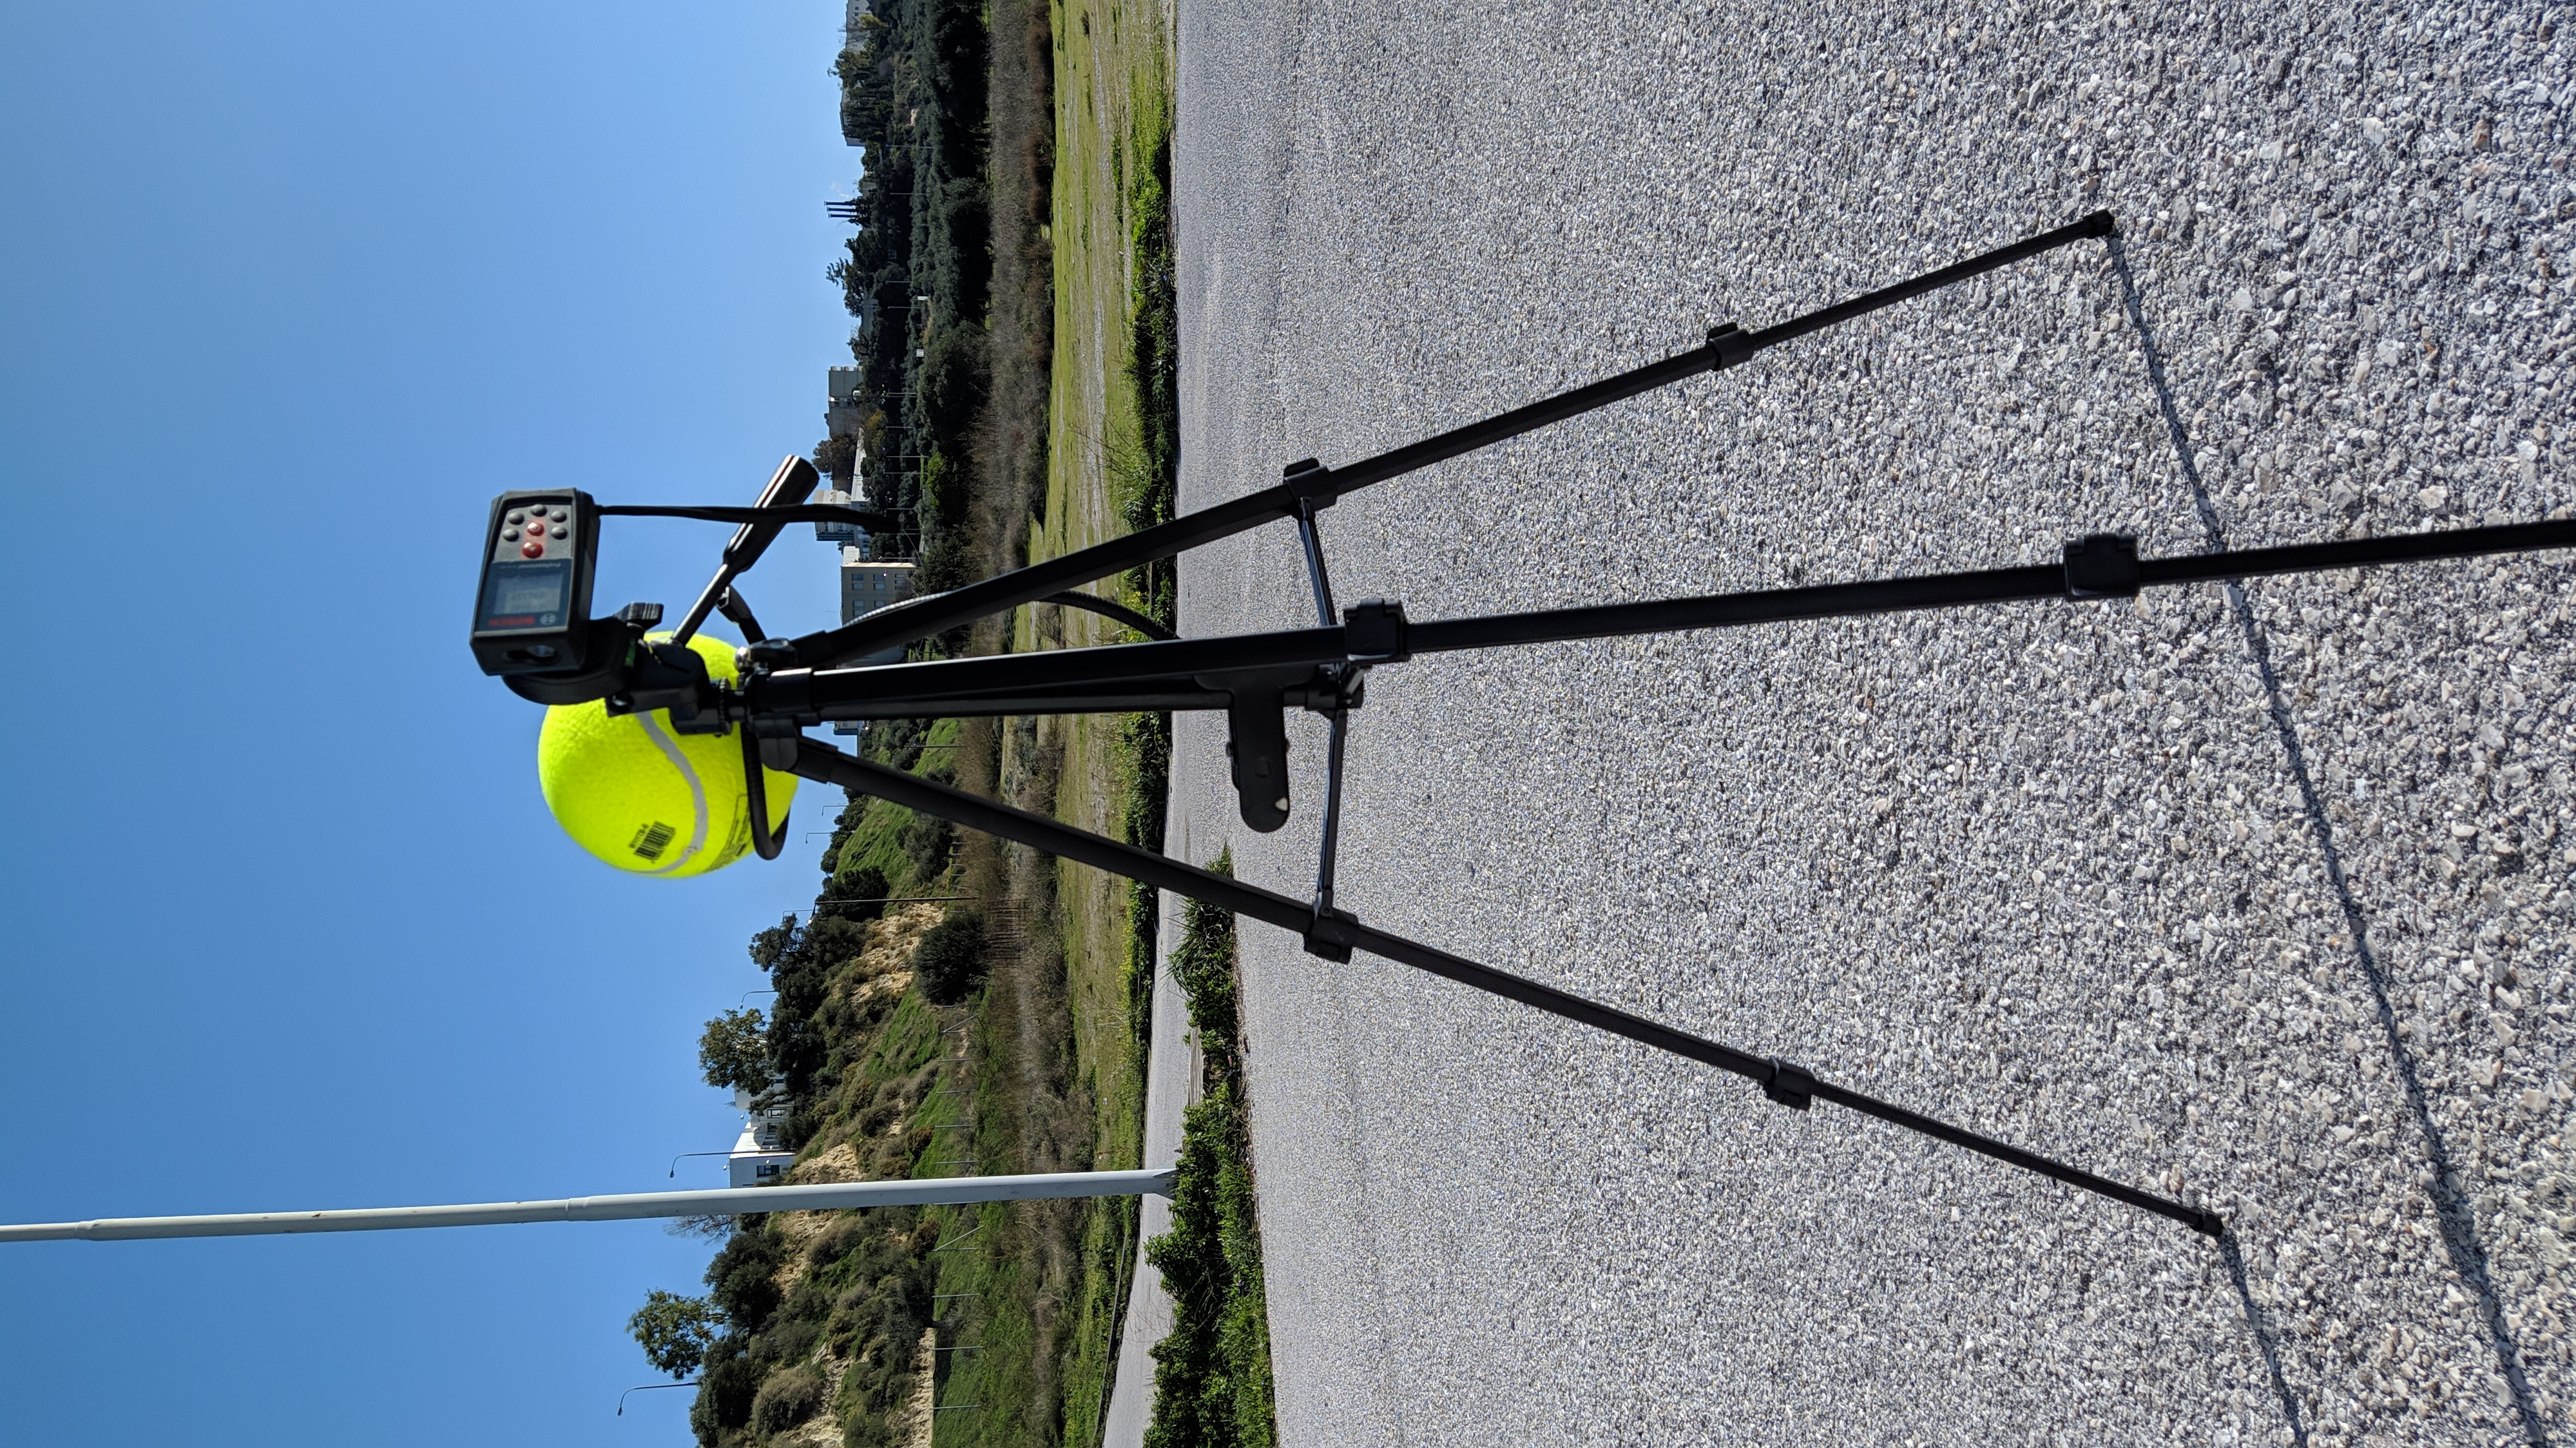
\includegraphics[width=\linewidth, angle =-90]{../Images/Experiments-Results/testing.jpg}\\ \vspace{0.1cm}
      {(b) Κινούμενο αντικείμενο εκτίμησης θέσης μαζί με το όργανο μέτρησης απόστασης }
	\end{minipage}
	% -----------------
    \hfill \break
    \decoRule
    \CaptionBasedwithURL{Εξοπλισμός που χρησιμοποιήθηκε στην πρώτη εξωτερική πειραματική φάση} 
    \label{fig:node-testing-env}
\end{figure}

Τα δύο αυτά αντικείμενα τοποθετήθηκαν το ένα απέναντι από το άλλο όπως φαίνεται στην \Fig{single-test-bench-side-view}, και πάρθηκαν μετρήσεις απόστασης για διαφορετικές γωνίες όπως φαίνεται στην 
\Fig{single-test-bench-angles}. Ταυτόχρονα, το σύστημα κατά την διάρκεια της διαδικασίας, ήταν σε πλήρη λειτουργία, και πραγματοποιούσε ανίχνευση και εκτίμηση της απόστασης του αντικειμένου από την κάμερα. Στη
\Sect{expe-single-3d} παρουσιάζονται τα πειραματικά αποτελέσματα των μετρήσεων αυτής της διαδικασία, ενώ στη 
\Sect{single-expe-system} παρουσιάζονται οι ανάγκες λειτουργίας από την σκοπιά του ε\-νσω\-μα\-τω\-μέ\-νου συστήματος.

\FigCaptLabelBasedURL{../Images/Experiments-Results/side.jpg}
{Χωρική τοποθέτηση του υπό ελέγχου συστήματος και αντικειμένου εκτίμησης θέσης}%
{single-test-bench-side-view}%
<0.8>

\FigCaptLabelBasedURL{../Images/Experiments-Results/testbench.png}
{Αναπαράσταση των θέσεων στις οποίες έγιναν οι μετρήσεις του πειράματος}%
{single-test-bench-angles}%
<0.6>

Όπως φαίνεται στην \Fig{node-testing-env} (b), το object το οποίο πρόκειται να εντοπίσουμε βρίσκεται σε τρίποδο, για μεγαλύτερη ευκολία των μετρήσεων, ενώ στο πλάγιο μέρος γίνεται διακριτό το όργανο που χρησιμοποιήθηκε για τον υπολογισμό της απόστασης μεταξύ των δύο αντικειμένων. Το όργανο αυτό είναι το laser range finder της Bosch GLM 40 - \Fig{bosch-range-estimator} - με δυνατότητες μέτρησης $0.15-40.00 m$ και απόκλιση μετρήσεων $\pm1.5mm$

Για τον υπολογισμό των διάφορων γωνιών από τις οποίες θα γινόντουσαν μετρήσεις, χρησιμοποιήθηκε το όργανο μέτρησης γωνιών όπως φαίνεται στην \Fig{single-test-bench-top-view}. Ενώ οι μετρήσεις που στην συνέχεια θα αναγερθούν αφορούν δεδομένα από γωνίες [$-20\si{\degree},-10\si{\degree},~0\si{\degree},~10\si{\degree},~20\si{\degree}$]\footnote{Λόγω του διαφορετικού ύψους μεταξύ της θέσης που μετρήθηκαν οι γωνίες και της κάμερας, δεν είναι οι ίδιες με αυτές που ανιχνεύονται στο x άξονα της εικόνας} και αποστάσεις μέτρησης ανά 50cm μέχρι τα 5m (εκτός από την κεντρική ευθεία στην οποία έγιναν μετρήσεις μέχρι περίπου τα 8m).

\FigCaptLabelBasedURL{../Images/Experiments-Results/glm40.jpg}
{Το ψηφιακό λέιζερ μέτρησης απόστασης που χρησιμοποιήθε (Bosch GLM 40)}%
{bosch-range-estimator}%
<0.4>%
(https://www.howetools.co.uk/bosch-glm-40-aaa-batteries-laser-range-finder)

\FigCaptLabelBasedURL{../Images/Experiments-Results/node-top-view.jpg}
{Υπολογισμός των γωνιών με χρήση εργαλείου μέτρησης γωνίας}%
{single-test-bench-top-view}%
<0.9>

% -------------------------------------------------------------
\subsection{Απόδοση του συστήματος} \label{sec:single-expe-system}

Πριν αναφερθούν τα δεδομένα που συλλέχθηκαν ως προς την απόδοση του συστήματος, θα αναφερθούν κάποια από τα 
χαρακτηριστικά λειτουργίας του. Η υλοποίηση του συστήματος έγινε σε C++. Δημιουργήθηκαν συνεπώς Function-like macros για εξαγωγή και αποθήκευση χρήσιμων πληροφοριών του συστήματος. Οι πληροφορίες που συλλέχθηκαν, αναφέρονται σε αυτήν την ενότητα, και σχετίζονται με τις επεξεργαστικές και ενεργειακές ανάγκες του συστήματος, η μνήμη μου χρειάζεται για να λειτουργήσει, και άλλες σημαντικές πληροφορίες.

Πρώτη από αυτές τις πληροφορίες είναι οι επεξεργαστικές ανάγκης του, όπου στην \Fig{cpu-usage-experiment-example}
φαίνονται τα δεδομένα που συλλέχθηκαν κατά την διάρκεια ενός από τα πειράματα. 

\FigCaptLabelBasedURL{../Images/Experiments-Results/raspberry-exp-cpu.png}
{Επεξεργαστική ισχύς του συστήματος}%
{cpu-usage-experiment-example}%
<1>

Μία ακόμα χρήσιμη μετρική είναι αυτή της μνήμης που χρησιμοποιεί το σύστημα, στην \Fig{ram-usage-experiment-example}
παρουσιάζεται η συγκεκριμένη πληροφορία. Από αυτό το διάγραμμα μπορούμε να παρατηρήσουμε ότι για την συγκεκριμένη υλοποίηση το σύστημα δεν έχει μεγάλες ανάγκες μνήμης\footnote{Έχοντας αυτήν την πληροφορία, μπορούμε να μεταβούμε σε επιλογή Embedded Linux System με μικρότερη μνήμη, που σημαίνει μικρότερο κόστος ανά node συστήματος}.
\FigCaptLabelBasedURL{../Images/Experiments-Results/raspberry-exp-ram.png}
{Ανάγκες μνήμης του συστήματος}%
{ram-usage-experiment-example}%
<1>

Το σύστημα αυτό σχεδιάζεται, με γνώμονα μελλοντικά να χρησιμοποιηθεί σε drones, συνεπώς οι ενεργειακές απαιτήσεις του είναι σημαντικές. Για αυτό τον λόγο ε\-ξά\-χθη\-καν και δεδομένα σχετικά με την κατανάλωση του συστήματος\footnote{Στις συγκεκριμένες γραφικές, μέχρι το 80s το σύστημα είναι σε idle mode, ενώ από εκεί και έπειτα είναι σε πλήρη λειτουργία} - \Fig{power-usage-experiment-example}. Με την μέγιστη κατανάλωση που παρατηρήθηκε από τροφοδοσία μέσω power bank κατά την διάρκεια δοκιμών είναι τα 10Watt, ενώ τάση τροφοδοσίας είναι τα 5Volt.
\FigCaptLabelBasedURL{../Images/Experiments-Results/raspberry-exp-power.png}
{Ενεργιακές απαιτήσεις συστήματος}%
{power-usage-experiment-example}%
<1>

Σημαντικός παράγοντας της απόδοσης ενός επεξεργαστή, είναι η θερμοκρασία του, καθώς αν είναι αυξημένη μπορεί η απόδοση να μειωθεί λόγω thermal throttling. Για αυτό συλλέχθηκε επίσης πληροφορία για την θερμοκρασία του επεξεργαστή - \Fig{temp-usage-experiment-example}. 
\FigCaptLabelBasedURL{../Images/Experiments-Results/raspberry-exp-temp.png}
{Θερμοκρασίες συστήματος έχοντας σε χρήση το fan του breakout board}%
{temp-usage-experiment-example}%
<1>

Ενώ τελευταία, αλλά εξίσου σημαντική μετρική, είναι ο υπολογισμός του χρόνου που χρειάζεται το σύστημα ανίχνευσης του αντικειμένου, για κάθε δευτερόλεπτο χρήσης του συστήματος, και παρουσιάζεται στην \Fig{hsv-calc-dur-experiment-example}.
\FigCaptLabelBasedURL{../Images/Experiments-Results/raspberry-exp-hsv-dur.png}
{Χρόνος του object detection μέσα σε κάθε δευτερόλεπτο χρήσης του συστήματος}%
{hsv-calc-dur-experiment-example}%
<1>

%----------------------------------------------------------------------

\subsection{Λαμβανόμενα δεδομένα και απεικόνιση} \label{sec:expe-single-3d}

Πριν αναφερθούν τα δεδομένα που λήφθηκαν κατά το πείραμα, είναι σημαντικό να γίνει κατανοητή η εξάρτηση pixel-απόστασης της σχέσης \EqNum{distance-from-object-pixels} που αναλύθηκε στο προηγούμενο κεφάλαιο και χρησιμοποιείται για το range estimation του αντικειμένου.

Η \Fig{pixel-dist-rel} παρουσιάζει την παραπάνω αναλογία, για τις παραμέτρους της κάμερας που χρησιμοποιήθηκε, σε αναλύσεις 1280x720 pixels.

\FigCaptLabelBasedURL{../Images/Experiments-Results/pixels-dist-rel.png}
{Εξάρτηση του μεγέθους του αντικειμένου σε pixel με απόσταση αντικειμένου από την κάμερα}%
{pixel-dist-rel}%
<1>

Αυτό που μπορούμε να παρατηρήσουμε είναι, ότι δεν είναι γραμμική. Όμως, μπορεί να προσεγγιστεί σε ένα υποσύνολο του πεδίο ορισμού της, με γραμμικό τρόπο. Αυτό σημαίνει ότι για σχετικά μεγάλες ακτίνες η μεταβολή σε pixel επιφέρει μικρές με\-τα\-βο\-λές στην απόσταση, ενώ για μικρές ακτίνες επιφέρει μεγάλες μεταβολές της απόστασης. 

Για λόγους πληρότητας θα δοθούν τρία παραδείγματα. Σε πολύ μικρές ακτίνες - λόγου χάρη για αντικείμενο ακτίνας 10 pixel - η εκτιμώμενη απόσταση είναι 12.4m, ενώ, αν το αντικείμενο εκτιμούσαμε ότι είχε ακτίνα 11 pixel, τότε η απόσταση θα ήταν 11.27m. Ως αποτέλεσμα, σε αυτήν την περίπτωση το 1 pixel σφάλματος του αντικειμένου στο image plane να καταλήγει σε 1.13m σφάλματος της εκτιμώμενης απόστασης στον φυσικό κόσμο. Για λίγο μεγαλύτερες ακτίνες, όπως για 50 pixel, η εκτιμώμενη απόσταση είναι 2.48m. Αν όμως για αυτή την ακτίνα του αντικείμενου είχαμε σφάλμα 1 pixel - δηλαδή μέτρηση 51 pixel - τότε η εκτιμώμενη απόσταση θα ήταν τα 2.43m, με τελικό σφάλμα τα 5cm σε αυτήν την περίπτωση. Τέλος, σε αρκετά μεγαλύτερες ακτίνες, με τα 100 pixel ως αναφορά, έχουμε εκτιμώμενη α\-πό\-στα\-ση τα 1.24m, ενώ, σε περίπτωση που η ακτίνα μας έχει 1 pixel διαφορά από την πραγματικότητα - δηλαδή έστω 101 pixels - και τα 1.22m εκτιμώμενη απόσταση, καταλήγουμε σε 2cm σφάλμα. Αυτό που βγαίνει ως συμπέρασμα από αυτήν την σχέση είναι ότι το τελικό σφάλμα εκτίμησης είναι σε άμεση εξάρτηση με το ποσοστό του image plane που καταλαμβάνει το αντικείμενο σε αυτό. 

Αφού έχει γίνει ξεκάθαρος αυτός ο περιορισμός, θα αναφερθούν τα δεδομένα που λήφθηκαν κατά την διάρκεια του πειράματος, από το node.
Αρχικά, στην \Fig{raspberry-exp-node-view} παρουσιάζεται στιγμιότυπο της αντιληπτικής ικανότητας - μεμονωμένης χρονικής στιγμής - του node, μαζί με τα διάφορα στάδια ε\-πε\-ξε\-ργα\-σίας, σε συνδυασμό με post-processing τρισδιάστατη απεικόνιση της μπάλας σε σχέση με την κάμερα (κάτω δεξιά στην εικόνα).

\FigCaptLabelBasedURL{../Images/Experiments-Results/node-view.png}
{Αντιληπτική ικανότητα μεμονωμένου κόμβου κατά την διάρκεια των δοκιμών, σε συνδυασμό με τρισδιάστατη απεικόνιση της μπάλας}%
{raspberry-exp-node-view}%
<1>

Οι γραφικές - \Fig{dist-experiment-example} και \Fig{angles-usage-experiment-example} - παρουσιάζουν τα raw data για την α\-πό\-στα\-ση και γωνίες που συλλέχθηκαν κατά την διάρκεια του πειράματος. Με την βοήθεια αυτών, μπορεί ακόμα και να φανεί η διαδρομή που ακολουθήθηκε κατά την διάρκεια του πειράματος. Επίσης, παρατηρείται να είναι σε ένα αρκετά μεγάλο ποσοστό κοντά στην πραγματική διαδρομή, με πολύ καλή προ\-σέ\-γγι\-ση για τον ε\-ντο\-πι\-σμό του αντικειμένου (όπως θα φανεί στην συνέχεια). Για τις οποίες, είναι σημαντικό όμως να αναφερθεί ότι τα spikes αναπαριστούν σημεία όπου δεν είχε γίνει ακριβές detection του object.

\begin{figure}[H]
  \centering
  \includegraphics[width=\linewidth]{../Images/Experiments-Results/raspberry-exp-dist.png}
  \decoRule
  \caption[Εκτίμηση απόστασης για κάθε δευτερόλεπτο χρήσης του συστήματος]{Εκτίμηση απόστασης για κάθε δευτερόλεπτο χρήσης του συστήματος (για 3 από τις 5 ευθείες)}
  \label{fig:dist-experiment-example}
\end{figure}


\begin{figure}[H]
  \centering
  \includegraphics[width=\linewidth]{../Images/Experiments-Results/raspberry-exp-angles.png}
  \decoRule
  \caption[Εκτίμηση γωνιών στους άξονες x και y για κάθε δευτερόλεπτο χρήσης του συστήματος]{Εκτίμηση γωνιών στους άξονες x και y για κάθε δευτερόλεπτο χρήσης του συστήματος (για 3 από τις 5 ευθείες)}
  \label{fig:angles-usage-experiment-example}
\end{figure}

Με βάση τις δύο παραπάνω γραφικές, για την εκτίμηση απόστασης και γωνιών οι οποίες αποτελούν scalar τιμές, μπορούμε σε συνδυασμό - με απλή γεωμετρία - να αναπαραστήσουμε στο τρισδιάστατο χώρο όλες τις εκτιμήσεις για τις θέσης του αντικειμένου και να καταλήξουμε σε ένα vector θέσης ως προς την κάμερα. Αυτό γίνεται προσπάθεια να επιτευχθεί στην \Fig{obj-3d-repre}. Θεωρητικά θα μπορούσαμε μόνο με αυτόν τον τρόπο να εντοπίσουμε το αντικείμενο στον \Abbr{3D} χώρο, για λόγους α\-ξιο\-πι\-στίας όμως ωθούμαστε στον προσδιορισμό της θέσης από δεδομένα πολλαπλών κόμβων - από swarm - ώστε σε μία πιθανή αποστολή να μην έχουμε single point of failure. 

\FigCaptLabelBasedURL{../Images/Experiments-Results/raspberry-exp-obj-3d.png}
{Τρισδιάστατη απεικόνιση των μετρήσεων για 3 από τις 5 ευθείες}%
{obj-3d-repre}%
<1>

%----------------------------------------------------------------------

\section{Δεδομένα πολλαπλών κόμβων}
Όπως αναφέρθηκε και στη \Sect{GPS}, η λειτουργία του \Abbr{GPS} - τουλάχιστον σε αυτήν την φάση - ήταν για λόγους πληρότητας της υλοποίησης, ώστε να γίνει εύκολο το integration ενός \Abbr{GPS} με μικρότερο σφάλμα - όπως \Abbr{RTK} \Abbr{GPS} - σε μελλοντική υλοποίηση. Για αυτόν τον λόγο στην συνέχεια αναφερόμαστε σε καθορισμένων συντεταγμένων nodes.

%----------------------------------------------------------------------

\subsection{Διαδικασία λήψης δεδομένων} \label{sec:multiple-nodes-data-collection}
Στην συνέχεια πραγματοποιήθηκαν μετρήσεις από πολλαπλά σημεία (κόκκινα τε\-τρά\-γω\-να στο διάγραμμα) για το ίδιο αντικείμενο όπως παρουσιάζεται στην \Fig{multiple-nodes-positions}.
Με αυτόν τον τρόπο, για την ίδια θέση της μπάλας (με μαύρο χρώμα στο διάγραμμα) θα μπορούσε να προσομοιωθούν - σε ένα πρώιμο τουλάχιστον στάδιο - τα δεδομένα που δημιουργούνται από πολλαπλούς κόμβους σε ένα σμήνος από drone. 

\FigCaptLabelBasedURL{../Images/Experiments-Results/nodes-pos.png}
{Απεικόνιση των θέσεων από τις οποίες πραγματοποιήθηκαν λήψεις, καθώς και οι θέσεις του αντικειμένου}%
{multiple-nodes-positions}%
<.8>

Για κάθε μία από αυτές τις θέσεις πάρθηκαν μετρήσεις απόστασης μέσω που laser range finder που αναφέρθηκε παραπάνω (\Fig{bosch-range-estimator}) καθώς επίσης καταγράφηκαν και οι εκτιμήσεις αποστάσεις που πραγματοποιήθηκαν από το σύστημα. Στο \Tabl{multiple-nodes-est-act-dist} παρουσιάζονται αναλυτικά αυτές οι μετρήσεις, ενώ στην \Fig{est-act-dist-figure} γίνεται οπτικοποίηση τους.

Επίσης, στην \Fig{multiple-nodes-perception} δίνεται παράδειγμα της αντιληπτικής ικανότητας του κάθε κόμβου, όταν έχει τοποθετηθεί στην θέση 2 (βλ. \Fig{multiple-nodes-positions}) το αντικείμενο.

% TABLE
\begin{table}[H]
  \caption[Πραγματικές αποστάσεις και εκτιμήσεις για κάθε γωνία λήψης]{Πραγματικές αποστάσεις και εκτιμήσεις για κάθε γωνία λήψης} \label{tab:multiple-nodes-est-act-dist}
  \centering
  \resizebox{0.9\textwidth}{!}{
    \begin{tabular}{ccccccccc}
        \toprule
        & \multicolumn{2}{c}{Node 1} & \multicolumn{2}{c}{Node 2} & \multicolumn{2}{c}{Node 3} & \multicolumn{2}{c}{Node 4} \\
        \midrule
    pos & Estimation      & Real     & Estimation      & Real     & Estimation      & Real     & Estimation      & Real     \\
    \midrule
    1   & 1.886 & 1.820 & 1.927 & 1.847 & 1.809 & 1.765 & 1.886 & 1.839 \\
    2   & 1.248 & 1.539 & 1.343 & 1.560 & 2.333 & 2.475 & 2.273 & 2.510 \\
    3   & 2.273 & 2.488 & 1.198 & 1.507 & 1.231 & 1.514 & 2.396 & 2.499 \\
    4   & 2.333 & 2.471 & 2.333 & 2.519 & 1.182 & 1.469 & 1.323 & 1.515 \\
    5   & 1.248 & 1.510 & 2.396 & 2.522 & 2.162 & 2.396 & 1.182 & 1.532 \\
    6   & 1.641 & 1.593 & 2.162 & 2.146 & 2.014 & 2.040 & 1.555 & 1.617 \\
    7   & 1.502 & 1.473 & 1.970 & 1.927 & 2.162 & 2.157 & 1.773 & 1.870 \\
    8   & 1.611 & 1.627 & 1.672 & 1.643 & 2.110 & 2.071 & 2.061 & 2.139 \\
    9   & 1.847 & 1.914 & 1.528 & 1.478 & 1.809 & 1.831 & 2.110 & 2.223 \\
    10  & 2.061 & 2.129 & 1.611 & 1.610 & 1.583 & 1.568 & 2.110 & 2.155 \\
    11  & 2.162 & 2.209 & 1.886 & 1.919 & 1.453 & 1.427 & 1.886 & 1.877 \\
    12  & 2.162 & 2.138 & 2.110 & 2.168 & 1.528 & 1.547 & 1.611 & 1.591 \\
    13  & 1.847 & 1.837 & 2.273 & 2.225 & 1.773 & 1.836 & 1.528 & 1.488 \\
    \bottomrule
    \end{tabular}
}
\end{table}

\begin{figure}[H]
  \centering
  \includegraphics[width=0.9\linewidth]{../Images/Experiments-Results/nodes-estimations.png}
  \decoRule
  \caption[Γραφική αναπαράσταση της εκτίμησης θέσης - πραγματικής απόστασης]{Γραφική αναπαράσταση της εκτίμησης θέσης - πρα\-γμα\-τι\-κής απόστασης (Σύμφωνα με τα δεδομένα του \Tabl{multiple-nodes-est-act-dist}, όπου \textcolor{blue}{o} οι εκτιμήσεις και \textcolor{red}{x} οι πραγματικές αποστάσεις)}
  \label{fig:est-act-dist-figure}
\end{figure}

Από τις παραπάνω μετρήσεις καταλήγουμε σε συνολικό μέσο όρο σφάλματος τα 0.0974 m. Αν διαχωρίσουμε το σφάλμα, με βάση τις εξωτερικές (2-5) και εσωτερικές (1 και 6-13) θέσεις τότε μπορούμε να καταλήξουμε σε δύο επιπλέον σφάλματα. Για τις εξωτερικές ο μέσος όρος των σφαλμάτων είναι τα 0.2230m ενώ για τις εσωτερικές τα 0.0686m. Ο λόγος που συμβαίνει αυτό, σχετίζεται με την παραμόρφωση που προκαλεί ο φακός της κάμερας (με μεγαλύτερες επιδράσεις προς τα άκρα του image plane), και δεν έγινε εφικτό μέσω του calibration να διορθωθεί.

\FigCaptLabelBasedURL{../Images/Experiments-Results/multiple-nodes/combined/low-res/p2.png.low.png}
{Αντιληπτική ικανότητα από κάθε γωνία λήψης για την θέση 2}%
{multiple-nodes-perception}%
<1>

%----------------------------------------------------------------------

\subsection{Εκτίμηση θέσης και απεικόνιση}
Έχοντας συλλέξει τα δεδομένα που αναφέρθηκαν στη \Sect{multiple-nodes-data-collection}, μπορούσε να χρησιμοποιηθεί ο φορμαλισμός που περιγράφηκε στη \Sect{implementation-obj-mult} για την εκτίμηση της θέσης στον τρισδιάστατο χώρο. 

Χρησιμοποιήθηκαν 4 nodes - με ένα από αυτά να αποτελεί ταυτόχρονα χρέη master και worker node - όπου έστελναν στο σύστημα επαναλαμβανόμενα τα ranges και positions του κάθε node που αναφέρθηκαν παραπάνω, με τον τρόπο που περιγράφηκε στο προηγούμενο κεφάλαιο. Αφού το master λάβει τα πακέτα και πραγματοποιήσει την επεξεργασία, χρησιμοποιεί \textbf{geometry\_msgs/Pose} - αποτελεί ένα από τις βασικές μορφές μηνυμάτων για θέση του \Abbr{ROS} - για να γνωστοποιηθεί στο δίκτυο την εκτίμηση της θέση της μπάλας.

Σύμφωνα με τα παραπάνω, στην \Fig{exp-topics-nodes} φαίνονται τα περιεχόμενα των topic κατά την διαδικασία του πειράματος, ενώ στην \Fig{multi-exp-pos-estimations} μπορούμε να δούμε συνδυαστικά τις γραφικές, στις οποίες παρουσιάζονται οι θέσεις που βρισκόταν το αντικείμενο, καθώς και οι εκτιμήσεις της θέσης που τελικά προέκυψαν.

Από τις εκτιμήσεις και τις ακριβής θέσεις, μπορούμε τελικά να υπολογίσουμε το συνολικό σφάλμα του συστήματος. Για το οποίο καταλήγουμε, ότι το συνολικό σφάλμα εκτίμησης θέσης από το σμήνος να είναι τα 0,1159m.

\begin{figure} [H]
	\centering
	% -----------------
    \begin{minipage}{.5\textwidth}
      \centering
      \includegraphics[width=0.9\linewidth]{../Images/Experiments-Results/nodes-pos-with-est-up.png}\\
      {(a) Top View}
    \end{minipage}%
    % -----------------
    \begin{minipage}{.5\textwidth}
      \centering
      \includegraphics[width=.9\linewidth]{../Images/Experiments-Results/nodes-pos-with-est-side.png}\\
      {(b) Side View}
	  \end{minipage}
	% -----------------
  \begin{minipage}{\textwidth}
    \centering
    \includegraphics[width=.8\linewidth]{../Images/Experiments-Results/nodes-pos-with-est-angle.png}\\
    {(C) Angled View}
  \end{minipage}
% -----------------
    \hfill \break
    \decoRule
    \caption[Εκτίμηση θέσης του αντικειμένου.]{Εκτίμηση θέσης του αντικειμένου. Με \textcolor{black}{\LARGE$\circ$} είναι οι θέσεις στις οποίες τοποθετήθηκε το αντικείμενο ενώ με \textcolor{green}{\LARGE$\circ$} είναι οι θέσεις που έγινε εκτίμηση ότι βρίσκεται} %\CaptionBasedwithURL{Possible Embedded Linux Systems} 
    \label{fig:multi-exp-pos-estimations}
\end{figure}

\FigCaptLabelBasedURL{../Photos/topics.wr.png}
{Μέρος των εν λειτουργία nodes/topics, καθώς και απεικόνιση των πληροφοριών που αποστέλλουν στα topics τα 4 nodes, μαζί με την εκτίμηση της θέσης από τον master.}%
{exp-topics-nodes}%
<1>

%----------------------------------------------------------------------

\section{Επαλήθευση προσδιορισμού ID}
Όπως αναφέρθηκε στη \Sect{id-estimation} χρησιμοποιούμε την συχνότητα με την οποία αναβοσβήνει το led για τον καθορισμό του ID\footnote{Βίντεο από την διαδικασία του πειράματος μπορεί να βρεθεί στο \cite{experiment-blink-video}}. Σημαντικός παράγοντας για την επιλογή της συχνότητας είναι το frame-rate της κάμερας με την οποία δειγματοληπτούμε. 

Από το Nyquist–Shannon sampling theorem γνωρίζουμε ότι πρέπει να ισχύει $f_s > 2f_{max}$ μεταξύ της συχνότητας δειγματοληψίας και της μέγιστης συχνότητας σε ένα σήμα. Στην πράξη, είναι συχνό φαινόμενο να επιλέγουμε να διαφέρουν ακόμα και μία τάξη μεγέθους στην παραπάνω ανίσωση. Λόγω των 30fps της κάμερας καταλήγουμε να έχουμε ανά περίπου 33.33ms νέο καρέ, συνεπώς επιλέχθηκε ο χρόνος για τον οποίο θα είναι ενεργοποιημένο το led να είναι τα 70ms ώστε να καταγράφεται από τουλάχιστον 2 καρέ η ενεργοποίηση του. 

Για τις περιόδους ανάλογα με το ID επιλέχθηκαν οι χρόνοι 500ms για ID = 1, 1500ms για ID = 2, 2500ms για ID = 3, κλπ., ώστε να υπάρχει ένα περιθώριο 1000ms για πιθανά σφάλματα μεταξύ των μετρήσεων. 

Η \Fig{id-osci-samples} παρουσιάζει τους παλμούς στους οποίους ενεργοποιείται το led, και κρατάμε αποδεκτό το ID = 1 για durations μεταξύ των παλμών durations <= 1000ms, όμοια για ID = 2 έχουμε 1000ms < duration <= 2000ms, κλπ.

\begin{figure} [H]
	\centering
	% -----------------
    \begin{minipage}{.5\textwidth}
      \centering
      \includegraphics[width=0.9\linewidth]{../Images/Experiments-Results/node-pulses-0_5sec.png}\\
      {(a) Συχνότητα του led για ID = 1}
    \end{minipage}%
    % -----------------
    \begin{minipage}{.5\textwidth}
      \centering
      \includegraphics[width=.9\linewidth]{../Images/Experiments-Results/node_pulses_1_5sec.png}\\
      {(b) Συχνότητα του led για ID = 2}
	  \end{minipage}
% -----------------
    \hfill \break
    \decoRule
    \caption[Παράδειγμα δύο εκ των τεσσάρων συχνοτήτων για την λειτουργία του led που επιλέχθηκαν.]{Παράδειγμα δύο εκ των τεσσάρων συχνοτήτων για την λειτουργία του led που επιλέχθηκαν.}%\CaptionBasedwithURL{Possible Embedded Linux Systems} 
    \label{fig:id-osci-samples}
\end{figure}

Τέλος, η \Fig{exp-led-freq} παρουσιάζει στιγμιότυπο κατά την διαδικασία επαλήθευσης της λειτουργίας, στο οποίο παρουσιάζεται τόσο το ID που εκτιμήθηκε όσο και το duration μεταξύ την παλμών.

\FigCaptLabelBasedURL{../Images/Experiments-Results/frequency-analysis.png}
{Στιγμιότυπο της διαδικασίας πείραματος, κατά την διάρκεια καθορισμού του ID του αντικειμένου με βάση την συχνότητα που αναβοσβήνει το led}%
{exp-led-freq}%
<.8>

Από τα παραπάνω πειράματα, δείχνεται ότι είναι εφικτός ο προσδιορισμός της θέσης της μπάλας. Παρόλα αυτά, λόγω των περιορισμών που αναφέρθηκαν, σε αυτήν την μορφή που βρίσκεται ακόμα το σύστημα, συμπεραίνουμε ότι πρα\-γμα\-το\-ποι\-εί τις βέλτιστες προσεγγίσεις της θέσης, όταν το αντικείμενο ανιχνεύεται περίπου στο μέσω του image plane σε αποστάσεις κάτω των 5m.

Ακόμα, ενώ μπορεί να προσδιοριστεί μοναδικά το ID του αντικειμένου που εντοπίζεται, είναι φανερό ότι ο χρόνος που χρειάζεται ώστε αξιόπιστα να καθοριστεί αυτό\udot δεν είναι πεπερασμένος και μπορεί να χρειαστεί μερικά δευτερόλεπτα. Ο οποίος εξαρτάται από το πλήθος των μοναδικών ID που θέλουμε να ανιχνεύσουμε, το duration που έχει προεπιλεχθεί για κάθε ID, καθώς και τον αριθμό των επαναλήψεων που επιθυμούμε να επαναλάβουμε την παραπάνω διαδικασία ώστε πριν προσδιορίσουμε το ID ώστε αξιόπιστα να έχουμε εκτίμηση του.






   % Design Verification and Performance Results
\chapter{Conclusions and Future Work} % Main chapter title
\label{chap:Chapter7}
%\epigraph{The key to artificial intelligence has always been the representation.” }{\textit{Jeff Hawkins}}
   % Future work

%----------------------------------------------------------------------------------------
%	THESIS CONTENT - APPENDICES
%----------------------------------------------------------------------------------------

\appendix % Cue to tell LaTeX that the following "chapters" are Appendices

% Include the appendices of the thesis as separate files from the Appendices folder
% Uncomment the lines as you write the Appendices

% Todo: comment out if not needed	
% \include{Appendices/AppendixA}
% \include{Appendices/AppendixB}
% \include{Appendices/AppendixC}

%----------------------------------------------------------------------------------------
%	BIBLIOGRAPHY
%----------------------------------------------------------------------------------------

\cleardoublepage
\phantomsection
\addcontentsline{toc}{chapter}{References}
\printbibliography[keyword={References}, title={References}]
\printbibliography[keyword={Link}, title={External Links}]

% Personal last page
\cleardoublepage
\thispagestyle{plain}
\thispagestyle{empty} 
\null\vfil
\begin{center}{\Large\slshape Last Page}\end{center}
\vfil\null
%----------------------------------------------------------------------------------------

\end{document}
